\documentclass[12pt]{book}

\usepackage[top=1in, bottom=1in, left=1.5in, right=1.5in, letterpaper]{geometry}
\usepackage{booktabs}
\usepackage{setspace}
\usepackage{trackchanges}
\usepackage{fancyhdr}
\usepackage{etoolbox}
\usepackage{lipsum}
\usepackage{amsmath}
\usepackage{listings}
\usepackage{wasysym}
\usepackage{float}
\usepackage[font=small,labelfont=bf]{caption}
\usepackage[caption=false,font=footnotesize,format=hang]{subfig}
\usepackage{pgfplots}
\pgfplotsset{compat=1.5}
\usetikzlibrary{plotmarks,arrows}
\tikzset{>=latex}
%\usepgfplotslibrary{colorbrewer}
\usepackage[absolute,overlay]{textpos}
\usepackage{graphicx}
\usepackage{lmodern}
\usepackage{longtable}
\usepackage{xfrac}
\usepackage{siunitx}
\usepackage[style=ieee,backend=biber]{biblatex}
\addbibresource{references.bib}
\usepackage[hidelinks, bookmarks=true]{hyperref}
\usepackage{bookmark}
\usepackage{algorithmicx}
\usepackage{algpseudocode}
\usepackage[chapter]{algorithm}
%\usepackage{droid}
\usepackage[T1]{fontenc}
\usepackage[titletoc]{appendix}
\usepackage[section]{placeins}

% add a "DRAFT" watermark to everything
%\usepackage{draftwatermark}
%\SetWatermarkLightness{0.8}
%\SetWatermarkScale{1.5}

% set up SIunitsX
\sisetup{
	group-four-digits = true,
	group-separator = {,},
	%per=frac,
	%fraction=nice
	%fraction=sfrac
	%per-mode=symbol,
}
%\newcommand{\usd}[1]{\SI{#1}[\$\ensuremath{\,}]{}}
\newcommand{\percent}{\%}

% set up colours for plots
% these are based on mapping colours that should photocopy in black and white well
\definecolor{pc1}{HTML}{8DD3C7}
\definecolor{pc2}{HTML}{FDB462}
\definecolor{pc3}{HTML}{FB8072}
\definecolor{pc4}{HTML}{80B1D3}
\definecolor{pc5}{HTML}{B3DE69}
\definecolor{pc6}{HTML}{BEBADA}
\definecolor{pc7}{HTML}{FCCDE5}
\definecolor{pc8}{HTML}{D9D9D9}
\definecolor{pc9}{HTML}{FFFFB3}
\pgfplotscreateplotcyclelist{ColourPlotCycle}{%
solid,ultra thick,pc1,every mark/.append style={fill=pc1},mark=*\\%
solid,ultra thick,pc2,every mark/.append style={fill=pc2},mark=square*\\%
solid,ultra thick,pc3,every mark/.append style={fill=pc3},mark=diamond*\\%
solid,ultra thick,pc4,every mark/.append style={fill=pc4},mark=pentagon*\\%
solid,ultra thick,pc5,every mark/.append style={fill=pc5},mark=triangle*\\%
dashed,ultra thick,pc6,every mark/.append style={fill=pc6},mark=*\\%
dashed,ultra thick,pc7,every mark/.append style={fill=pc7},mark=square*\\%
dashed,ultra thick,pc8,every mark/.append style={fill=pc8},mark=diamond*\\%
dashed,ultra thick,pc9,every mark/.append style={fill=pc9},mark=pentagon*\\%
}
\pgfplotscreateplotcyclelist{SmoothColourPlotCycle}{%
solid,ultra thick,pc1\\%
solid,ultra thick,pc2\\%
solid,ultra thick,pc3\\%
solid,ultra thick,pc4\\%
solid,ultra thick,pc5\\%
dashed,ultra thick,pc6\\%
dashed,ultra thick,pc7\\%
dashed,ultra thick,pc8\\%
dashed,ultra thick,pc9\\%
}
\pgfplotscreateplotcyclelist{BarColourPlotCycle}{%
fill=pc1\\%
fill=pc2\\%
fill=pc3\\%
fill=pc4\\%
fill=pc5\\%
fill=pc6\\%
fill=pc7\\%
fill=pc8\\%
fill=pc9\\%
}

\definecolor{RdBuWhiteGrey}{RGB}{247,247,247}
\pgfplotsset{
	colormap={RdBu}{
		rgb255(0cm)=(5,48,97);
		rgb255(1cm)=(33,102,172);
		rgb255(2cm)=(67,147,195);
		rgb255(3cm)=(146,197,222);
		rgb255(4cm)=(209,229,240);
		rgb255(5cm)=(247,247,247);
		rgb255(6cm)=(253,219,199);
		rgb255(7cm)=(244,165,130);
		rgb255(8cm)=(214,96,77);
		rgb255(9cm)=(178,24,43);
		rgb255(10cm)=(103,0,31);
	}
}
\pgfplotsset{
	colormap={YlOrRd}{
		rgb255(0cm)=(128,0,38);
		rgb255(1cm)=(189,0,38);
		rgb255(2cm)=(227,26,28);
		rgb255(3cm)=(252,78,42);
		rgb255(4cm)=(253,141,60);
		rgb255(5cm)=(254,178,76);
		rgb255(6cm)=(254,217,118);
		rgb255(7cm)=(255,237,160);
		rgb255(8cm)=(255,255,204);
	}
}

% set up colours for schematics
\definecolor{tissueColour}{RGB}{251,185,130}
\definecolor{lesionColour}{RGB}{175,50,53}
\definecolor{fatColour}{RGB}{240,236,182}
\definecolor{boneColour}{RGB}{200,200,200}

% set up source code listing
\definecolor{mygreen}{rgb}{0,0.6,0}
\definecolor{mygray}{rgb}{0.5,0.5,0.5}
\definecolor{mymauve}{rgb}{0.58,0,0.82}

\lstset{ %
	backgroundcolor=\color{white},     % choose the background color; you must add \usepackage{color} or \usepackage{xcolor}
	basicstyle=\footnotesize\ttfamily, % the size of the fonts that are used for the code
	breakatwhitespace=false,           % sets if automatic breaks should only happen at whitespace
	breaklines=true,                   % sets automatic line breaking
	captionpos=t,                      % sets the caption-position to bottom
	commentstyle=\color{mygreen},      % comment style
	deletekeywords={...},              % if you want to delete keywords from the given language
	escapeinside={\%*}{*)},            % if you want to add LaTeX within your code
	extendedchars=true,                % lets you use non-ASCII characters; for 8-bits encodings only, does not work with UTF-8
	frame=L,                           % adds a frame around the code
	keepspaces=true,                   % keeps spaces in text, useful for keeping indentation of code (possibly needs columns=flexible)
	keywordstyle=\color{blue},         % keyword style
	morekeywords={*,...},              % if you want to add more keywords to the set
	numbers=left,                      % where to put the line-numbers; possible values are (none, left, right)
	numbersep=10pt,                     % how far the line-numbers are from the code
	numberstyle=\tiny\color{mygray},   % the style that is used for the line-numbers
	rulecolor=\color{black},           % if not set, the frame-color may be changed on line-breaks within not-black text (e.g. comments (green here))
	showspaces=false,                  % show spaces everywhere adding particular underscores; it overrides 'showstringspaces'
	showstringspaces=false,            % underline spaces within strings only
	showtabs=false,                    % show tabs within strings adding particular underscores
	stepnumber=2,                      % the step between two line-numbers. If it's 1, each line will be numbered
	stringstyle=\color{mymauve},       % string literal style
	tabsize=2,                         % sets default tabsize to 2 spaces
	title=\lstname                     % show the filename of files included with \lstinputlisting; also try caption instead of title
}

% align subfloats to the top of the float
%\captionsetup[subfloat]{position=top}

% highlight footnotes in red
\renewcommand\thefootnote{\textcolor{red}{\arabic{footnote}}}
% TODO: automate footnote command with \textcolor{red} in the footnote as well

% setup the bibliography
%\renewcommand\bibname{References}
\DefineBibliographyStrings{english}{%
	bibliography = {References}
}

% remove empty pages after \chapter commands
\let\cleardoublepage\clearpage

% set up our headers
\setlength{\headheight}{15.2pt}
\pagestyle{fancy}
\fancyhf{}
\renewcommand{\headrulewidth}{0pt}

\makeatletter
\renewcommand\chapter{\if@openright\cleardoublepage\else\clearpage\fi
                    \thispagestyle{fancyplain}% original style: plain
                    \global\@topnum\z@
                    \@afterindentfalse
                    \secdef\@chapter\@schapter}
\makeatother

% some utility commands
\newcommand{\comment}[1]{}
\newcommand{\x}[1]{}
\newcommand{\bibcomplete}[1]{}

% trackchanges editors
\addeditor{KH}
\addeditor{MFP}
\addeditor{WM}

% rename "Figure" to "Fig."
\def\figurename{Fig.}

% rename "Contents" to "Table of Contents"
\renewcommand*\contentsname{Table of Contents}

\begin{document}

\pdfbookmark{Title Page}{title}
\comment{\begin{center}

{\fontsize{14pt}{1em}\selectfont \textbf{University of Alberta}}
\vspace{3em}

{\fontsize{13pt}{1em}\selectfont Numerical Characterization of Ultrasound Elastography for the Early Detection of Deep Tissue Injuries}
\vspace{2em}

{\fontsize{10pt}{1em} by}
\vspace{1em}

{\fontsize{13pt}{1em} Kenton Hamaluik}
\vspace{5em}

{\fontsize{11pt}{1em} A thesis submitted to the Faculty of Graduate Studies and Research in partial fulfilment of the requirements for the degree of}
\vspace{3em}

{\fontsize{13pt}{1em} Master of Science}
\vspace{4em}

{\fontsize{13pt}{1em} Department of Mechanical Engineering}
\vspace{5em}

{\fontsize{11pt}{1em}\copyright\ Kenton Hamaluik \\
Winter 2014 \\
Edmonton, Alberta}
\vfill

{\fontsize{9pt}{1em} Permission is hereby granted to the University of Alberta Libraries to reproduce single copies of this thesis and to lend or sell such copies for private, scholarly or scientific research purposes only. Where the thesis is converted to, or otherwise made available in digital form, the University of Alberta will advise potential users of the thesis of these terms.
\vspace{1em}

The author reserves all other publication and other rights in association with the copyright in the thesis and, except as herein before provided, neither the thesis nor any substantial portion thereof may be printed or otherwise reproduced in any material form whatsoever without the author's prior written permission.}
\end{center}}

\begin{center}
	\vspace*{\fill}
	Numerical Characterization of Ultrasound Elastography for the Early Detection of Deep Tissue Injuries
	\vspace{1em}

	by
	\vspace{1em}

	Kenton David Hamaluik
	\vspace{6em}

	A thesis submitted in partial fulfillment of the requirements for the degree of
	\vspace{2em}

	Master of Science
	\vspace{6em}

	Department of Mechanical Engineering\\
	University of Alberta
	\vspace{10em}

	\copyright\ Kenton Hamaluik, 2014
	\vspace*{\fill}
\end{center}
\newpage

\setcounter{page}{1}
\pagenumbering{roman}
\doublespacing
\rfoot[\thepage]{\thepage}

\pdfbookmark{Abstract}{abstract}
\chapter*{Abstract}
	\doublespacing

	\note[KH]{Write abstract}
\newpage
\pdfbookmark{Preface}{preface}
\onehalfspacing
\chapter*{Preface}
	Chapter \ref{chap:quasi-static} of this thesis has been published as K. Hamaluik, W. Moussa, M. Ferguson-Pell, ``Numerical Characterization of Quasi-Static Ultrasound Elastography,'' \emph{IEEE Transactions on Medical Imaging}. I was responsible for the study design, data collection, and manuscript composition. W. Moussa and M. Ferguson-Pell were the supervisory authors and assisted with manuscript composition.
\newpage
\pdfbookmark{Dedication}{dedication}
\onehalfspacing
\chapter*{Dedication}
	This work was written for all those who have lovingly supported me throughout it's creation.

	To my mother Meridel, who instilled in me the desire to always better myself and persist through the greatest of difficulties. Even when things got difficult, you gently pushed me to continue even to your own detriment.

	To my late father David, who taught me about the world and inspired my combination of creativity, critical analysis, and work ethic. I wasn't able to finish before he left us, but I know he would be proud of what I accomplished in the end.

	To my beautiful wife Dennie, who has stood by me and loved me without condition in the face of adversity and struggle. Without you, I would have given up long ago. You supported me above all others and this work exists as much because of you as it does because of me.
\newpage
\pdfbookmark{Acknowledgements}{acknowledgements}
\onehalfspacing
\chapter*{Acknowledgements}
	This work reflects the endless days I have spent learning, researching, and growing throughout the past several years and would not have been possible without the gracious assistance of the considerable number of people supporting me.

	My supervisor, Dr. Walied Moussa has been a constant source of inspiration and learning for me. His enthusiam and tenacity for research became a model for this work early on in the process. I would like to thank him for providing me with this alongside all the resources and support I needed to complete this work.

	I would also like to thank my co-supervisor, Dr. Martin Ferguson-Pell for believing in me since I was an undergrad and continually providing me with opportunities to advance my learning. Despite his tremendous responsibilities, he always made time for me when I needed it and has always provided valuable input and guidance.

	I am incredibly grateful for the wonderful guidance, support, and supervision of the entire Project SMART Pressure Ulcer group along with the rest of the PIs and trainees of the Project SMART team. Their gentle leadership, kind friendship, and impressive ability continually inspired me to pursue my best and live up to their remarkable example.

	Lastly, I would like to thank my family and friends who have kept faith with me and my work since its inception while only marginally mocking me about my career choices.

	I truly stand as a dwarf upon the shoulders of giants.
\newpage
\tableofcontents
\clearpage

\listoftables
\clearpage

\listoffigures
\clearpage
\newpage
\pdfbookmark{Nomenclature}{nomenclature}
\chapter*{Nomenclature}
	\section*{Mathematical Symbols}
		\begin{longtable}[l]{ll}
			Symbol & Meaning \\
			\hline \endhead
			$\alpha$ & Acoustic absorption coefficient \\
			$\alpha_0$ & Power law prefactor \\
			$\sfrac{B}{A}$ & Acoustic nonlinearity parameter \\
			$b_i$ & Body force \\
			$b_r$ & Blurred lesion blur radius \\
			$b_\rho$ & Clustered lesion density \\
			$C$ & Elasticity tensor \\
			$c_0$ & Speed of sound \\
			$c_T$ & Shear wave speed \\
			$d$ & Lesion depth \\
			$d_f$ & Focal depth \\
			$\delta_{sep}$ & Co-located lesion separation distance \\
			$E$ & Young's modulus \\
			$E_{rel}$ & Lesion stiffness ratio \\
			$E_{lesion}$ & Young's modulus of lesion \\
			$E_{nom}$ & Nominal lesion stiffness ratio \\
			$E_{tissue}$ & Young's modulus of tissue \\
			$\varepsilon$ & Strain \\
			$\varepsilon_{app}$ & Transducer-applied strain \\
			$\varepsilon_{lesion}$ & Measured lesion strain \\
			$\varepsilon_{rel,measured}$ & Measured lesion strain ratio \\
			$\varepsilon_{rel,true}$ & True lesion strain ratio \\
			$\varepsilon_{tissue}$ & Measured tissue strain \\
			$F$ & Applied body forces \\
			$f$ & Ultrasound frequency \\
			$f_i$ & Applied load \\
			$G_m$ & Shear modulus of the $m^{\text{\tiny th}}$ branch of a Maxwell model \\
			$\Gamma$ & Boundary domain \\
			$h$ & Lesion altitude \\
			$I$ & Acoustic intensity \\
			$I_{SPPA}$ & Spatial peak pulse average intensity \\
			$I_{SPTA}$ & Spatial peak time average intensity \\
			$K$ & Bulk modulus \\
			$k$ & Wave number \\
			$\lambda$ & Lam\'{e} constant \\
			$\lambda$ & Ultrasound wavelength \\
			$MI$ & Mechanical index \\
			$MSE$ & Mean squared error \\
			$\mu$ & Lam\'{e} constant (shear modulus) \\
			$\mu$ & Mean value \\
			$n_c$ & Number of acoustic periods \\
			$\nabla$ & Del operator \\
			$P_r$ & Refractory pressure \\
			$P_{source}$ & Ultrasound transducer source pressure \\
			$p$ & Acoustic pressure \\
			$r_{lesion}$ & Lesion radius \\
			$r_{bl}$ & Clustered lesion radius \\
			$\rho$ & Acoustic density \\
			$\rho_0$ & Equilibrium density \\
			$S_M$ & Acoustic pressure source term \\
			$\diameter S$ & Lesion diameter \\
			$\diameter S$ & Visible Human lesion width \\
			$\sigma$ & Stress tensor \\
			$\sigma$ & Standard deviation \\
			$\sigma_0$ & Initial stress distribution \\
			$\sigma_{applied}$ & Stress applied to tissue \\
			$t_{inson}$ & Insonification time \\
			$\tau_m$ & Relaxation time of the $m^{\text{\tiny th}}$ branch of a Maxwell model \\
			$\vec{u}$ & Particle displacement \\
			$\vec{v}$ & Particle velocity \\
			$u_0$ & Initial displacement \\
			$v_{max}$ & Maximum tissue displacement in the axial direction \\
			$w_{active}$ & Total width of active transducer elements \\
			$y$ & Power law exponent \\
		\end{longtable}

	\section*{Abbreviations}
		\begin{longtable}[l]{ll}
			Abbreviation & Meaning \\
			\hline \endhead
			ARFI & Acoustic radiation force impulse \\
			DTI & Deep tissue injury \\
			IES & Intermittent electrical stimulation \\
			MRI & Magnetic resonance imaging \\
			NPUAP & National Pressure Ulcer Advisory Panel \\
			PU & Pressure ulcer \\
			SCI & Spinal cord injury \\
			USE & Ultrasound elastography \\
		\end{longtable}
\newpage

\setcounter{page}{1}
\pagenumbering{arabic}
\doublespacing
\rfoot[\thepage]{\thepage}

\chapter{Introduction}
	Ultrasound elastography is a relatively new ultrasonic imaging modality which utilizes traditional ultrasound waveforms to interrogate tissue stiffness rather than tissue echogenicity as is done in classic ultrasound imaging. The resulting tissue stiffness maps are referred to as elastograms, a terminology which will be used throughout this work. By examining displacement characteristics of tissue under load, the relative localized stiffness of the tissue may be ascertained. While regional tissue stiffness changes are to be expected due to the heterogeneous composition of generalized soft tissues, localized stiffness changes may be used as an indicator of tissue health \cite{gefen09} with relatively stiff tissues showing signs of rigor mortis and cell death and relatively soft tissues showing signs of tissue necrosis and decomposition. While ultrasound elastography has typically been used to investigate cancerous lesions this work seeks to use it as a means of detecting deep tissue injuries which as of the time of writing are not clinically detectable until they breach the surface of the skin.

	Before ultrasound elastography can be used clinically with any degree of certainty, the effect of numerous important parameters relating to the imaging modality must be understood and characterized. For example, chief parameters of interest include the depth of a lesion and its overall size---parameters which may immediately disqualify certain lesions from even being interrogated by diffused ultrasound beams and as a result would be invisible on the subsequent elastogram. Similarly, for the purposes of designing application-specific elastography transducers it becomes critical to fully understand the effect of transducer device parameters such as ultrasonic probing frequency and transducer f-number on the elastogram icanamage quality and lesion contrast. In order to properly use ultrasound elastography to detect, diagnose, and monitor formative and progressive deep tissue injuries it is crucial to first fully understand and characterize the technology for this specific use.

	\section{Objective}
		The broad objective of this work was to numerically characterize the use of ultrasound elastography to detect and monitor formative and progressive deep tissue injuries. When the effect of numerous interrogation parameters is understood, the technology may be evaluated on its feasibility and usefulness to detect deep tissue injuries, with the ultimate goal that ultrasound elastography be implemented clinically for detecting deep tissue injuries.

	\section{Motivation}
		According to the National Pressure Ulcer Advisory Board, deep tissue injuries are classified as a sub-category of pressure ulcers \cite{black11}. Pressure ulcers and subsequently deep tissue injuries are commonly suffered by people with limited mobility, such as those undergoing lengthy surgical procedures, the elderly, and those with spinal cord injuries \cite{allman95} with up to \unit{80}{\%} of people with spinal cord injuries developing at least one pressure ulcer in their lifetime \cite{salzberg96}. While traditional pressure ulcers form in a ``top-to-bottom'' pattern [??], deep tissue injuries form in a ``bottom-to-top'' pattern, whereby the injury starts deep below the skin surface---often at the bone-muscle interface \cite{kanno09}. This nature of not being externally visible until the wound has severely progressed makes deep tissue injuries exceedingly difficult to not only diagnose but also to prevent and treat.

		As of the time of writing, there is no clinically feasible method of detecting deep tissue injuries until they begin to damage the skin---even the National Pressure Ulcer Advisory Panel's description of them is largely based on their appearance after the fact \cite{npuap07}. With our inability to detect these forming injuries and subsequently implement deep tissue injury prevention and mitigation protocols, the injuries may eventually progress to form large subcutaneous cavities which eventually break through the surface and reveal themselves as stage III or IV pressure ulcers \cite{bouten03,oomens10}. \note[KH]{Needs more}

	\section{Methodology}
		In order to investigate the use of ultrasound elastography for the detection of deep tissue injuries, the technology must first be characterized and fully understood. While traditional experimentation provides an opportunity to work with physical subjects it can be severely limiting as absolute control over all investigated parameters is relinquished. Further, subject recruitment may present an insurmountable barrier to the execution of such a study. As such, in this exploratory work, various numerical models of the technology have been utilized to investigate the controlled effect of a broad number of parameters relating to each technology. Specifically, finite-element models of ultrasonic wave propagation in heterogeneous soft tissues have been developed. \annote[KH]{These models were coupled with various tissue strain estimation algorithms and utilized to carry out parametric studies on the detection sensitivity of ultrasound elastography with respect to various lesion and technological parameters.}{Holy wordy batman!} Chief parameters of interest include those related to the physical realities of deep tissue injuries such as lesion depth, size, and relative mechanical stiffness as well as parameters related to the design and development of appropriate ultrasonic transducers such as probing frequency, transducer f-number, etc.

	\section{Thesis Outline}
		In this work, three methods of ultrasonic elastogram image formation have been investigated: quasi-static ultrasound elastography, acoustic radiation force impulse imaging, and shear wave speed quantification. While all three methods may be used to interrogate tissue stiffness utilizing the principles of ultrasound physics.
\chapter{Literature Review}
\label{chap:litreview}
	In order to understand the need for a clinical method of detecting deep tissue injuries, the full scope and current state of the issue must be explored. To this end, the current state of the literature regarding deep tissue injuries, how they form, what factors characterize them, and how they are currently treated is explored here. In order to relate this disease to the detection modality proposed in this work, the mechanics and history of ultrasound elastography are also explored and related back to the problem at hand. The major gaps in the current literature regarding the use of ultrasound elastography for detecting and monitoring deep tissue injuries are presented as these gaps are what this work attempts to begin to fill.

	\section{Deep Tissue Injuries}
		Pressure ulcers, commonly referred to as ``bedsores'', are an extraordinarily large problem facing the health care system today. At least \SI{11}[\$]{billion} is spent in the United States of America alone treating approximately 500,000 injuries annually \cite{beckrich99,russo08} while only a minute fraction of that is spent toward pressure ulcer research \cite{zanca03}. Compared to hospital stays for all other conditions, patients with at least a secondary diagnosis of a pressure ulcer were more often discharged to a long-term care facility and more likely resulted in death \cite{russo08}. These injuries place an extremely significant burden on the people who suffer from them---pressure ulcers were found to have a profound impact on people's lives including: altering their physical, social, and financial status; changing their body image; losing independence and control; and subjecting them to the grieving process \cite{langemo00,baharestani94}. \note[KH]{I already mentioned this in the introduction, verbatim. Where should it go?}These debilitating wounds are often suffered by people with limited mobility such as those undergoing lengthy surgical procedures, the elderly, and those with spinal cord injuries (SCI) \cite{allman95}---approximately \SI{80}{\percent} of people with spinal cord injuries (SCI) will develop at least one pressure ulcer during their lifetime \cite{salzberg96} and approximately \SI{19}{\percent} of elderly patients in long-term care facilities will develop one \cite{freitas11}. Pressure ulcers exist throughout the entire health-care system and are often formed when undergoing hospitalization \cite{aronovitch99}. These injuries have a tendency to become chronic, non-healing wounds and many patients die from complications related to them \cite{jaul10}. Further, patients who have developed at least one pressure ulcer in their life are at a significantly greater risk of developing a second \cite{niazi97}. Pressure ulcers and deep tissue injuries generally form at the bone-muscle interface deep in the tissue \cite{kanno09} with approximately \SI{64}{\percent} occurring over the ischial tuberosities, trochanter, or sacrum \cite{garber03}. In general, these injuries are characterized by a some manner of tissue loss through necrosis of the tissue, though there is currently some debate on the exact nature of these wounds as well as the accuracy of the clinical descriptions attributed to them by the National Pressure Ulcer Advisory Panel (NPUAP).

		The NPUAP defines pressure ulcers as a ``localized injury to the skin and / or underlying tissue usually over a bony prominence, as a result of pressure, or pressure in combination with shear and / or friction'' and are generally staged according to a tiered system of increasing damage \cite{npuap07}. The various stages are depicted in Fig. \ref{fig:npuap-staging} and described as follows:

		\begin{figure*}[!t]
			\centering
			\subfloat[Normal tissue]{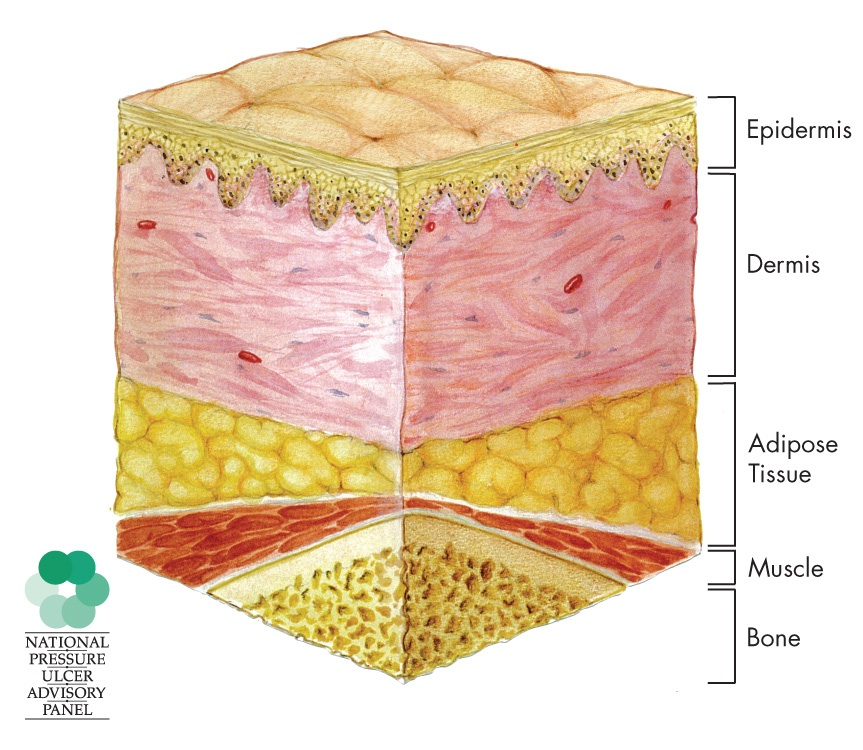
\includegraphics[width=0.3\textwidth]{assets/npuap/normal.png}\label{fig:npuap-normal}}

			\subfloat[Stage I]{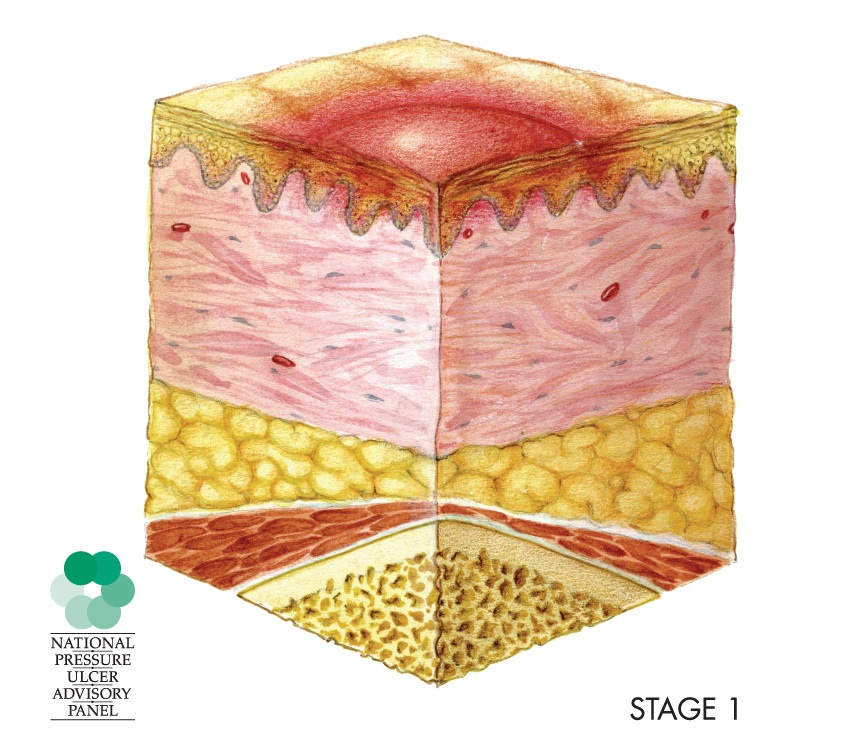
\includegraphics[width=0.3\textwidth]{assets/npuap/stage1.png}\label{fig:npuap-stage1}}
			\subfloat[Stage II]{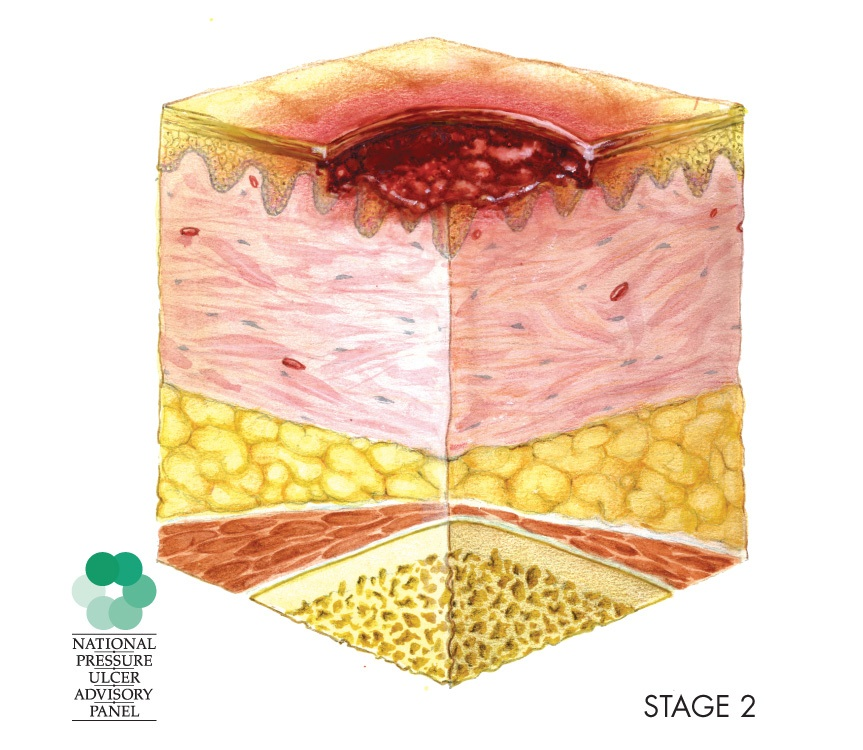
\includegraphics[width=0.3\textwidth]{assets/npuap/stage2.png}\label{fig:npuap-stage2}}
			\subfloat[Stage III]{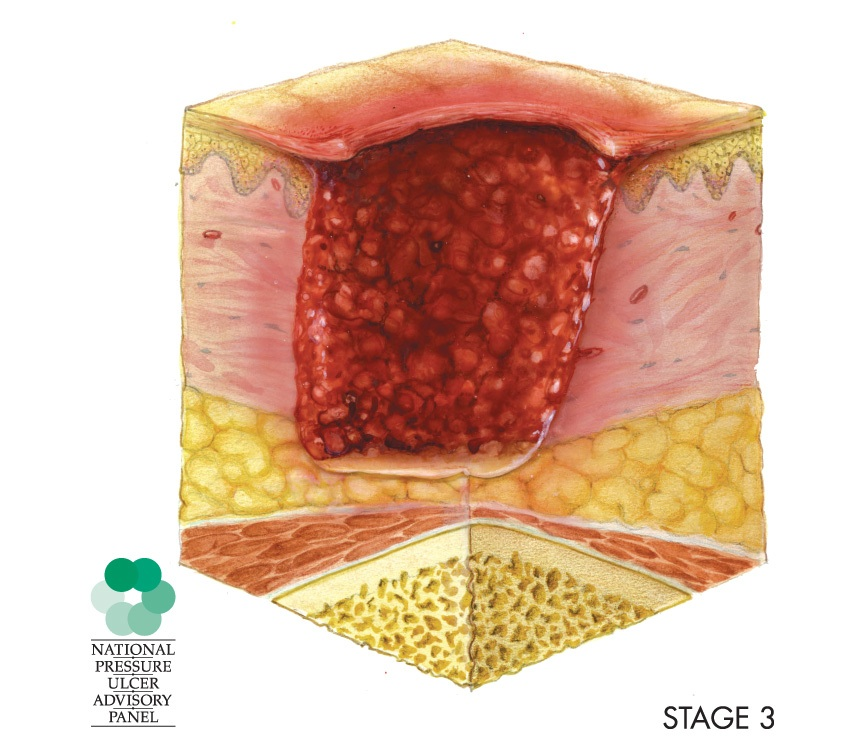
\includegraphics[width=0.3\textwidth]{assets/npuap/stage3.png}\label{fig:npuap-stage3}}

			\subfloat[Stage IV]{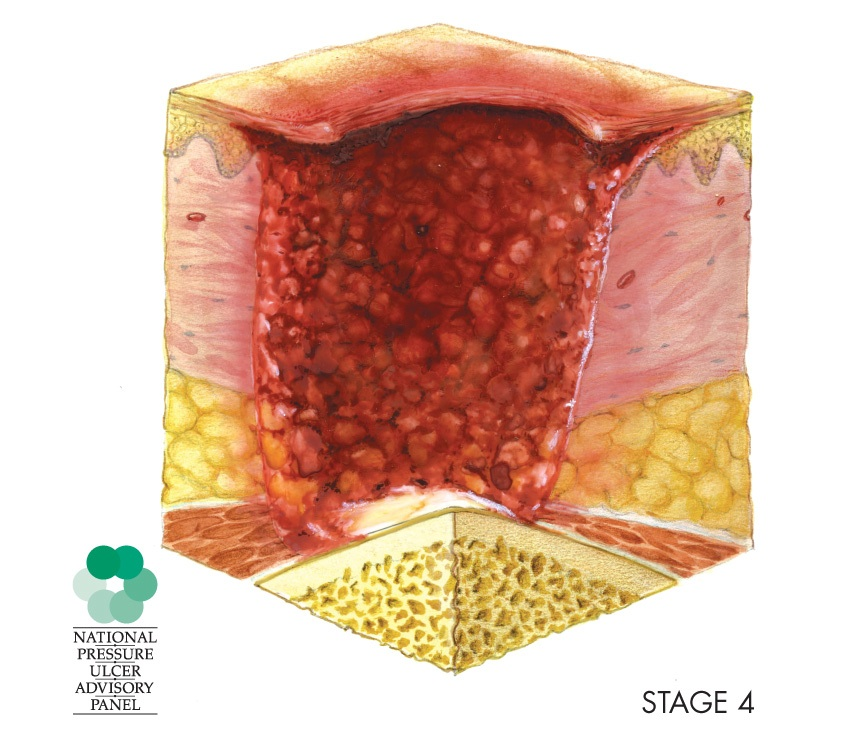
\includegraphics[width=0.3\textwidth]{assets/npuap/stage4.png}\label{fig:npuap-stage4}}
			\subfloat[Unstageable]{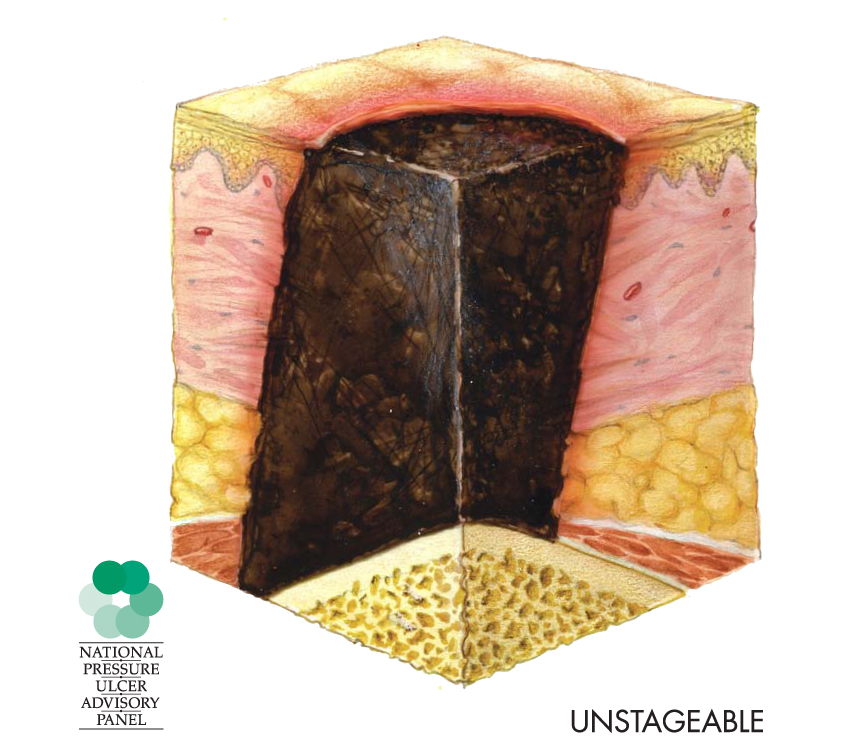
\includegraphics[width=0.3\textwidth]{assets/npuap/unstageable.png}\label{fig:npuap-unstageable}}
			\subfloat[Suspected DTI]{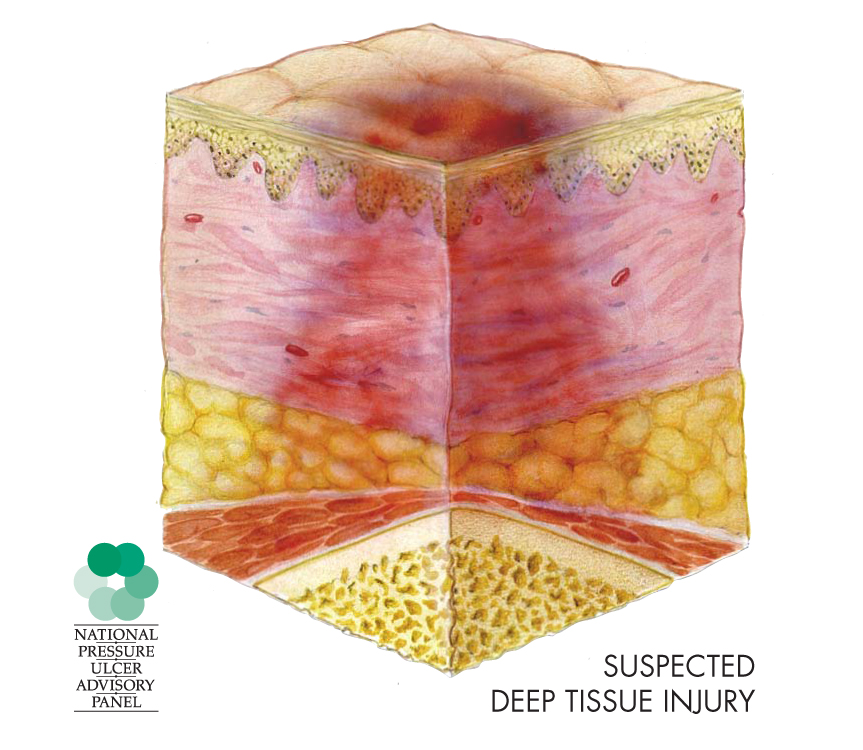
\includegraphics[width=0.3\textwidth]{assets/npuap/suspectedDTI.png}\label{fig:npuap-dti}}
			\caption[NPUAUP pressure ulcer staging guidelines]{The NPUAP staging guideline illustrations of the various stages / severities of pressure ulcers.}
			\label{fig:npuap-staging}
		\end{figure*}

		\begin{description}
			\item[Suspected Deep Tissue Injury] \hfill \\
				Purple or maroon localized area of discoloured intact skin or blood-filled blister due to damage of underlying soft tissue from pressure and / or shear. The area may be preceded by tissue that is painful, firm, mushy, boggy, warmer or cooler as compared to adjacent tissue.
			\item[Stage I] \hfill \\
				Intact skin with non-blanchable redness of a localized area usually over a bony prominence. Darkly pigmented skin may not have visible blanching; its colour may differ from the surrounding area.
			\item[Stage II] \hfill \\
				Partial thickness loss of dermis presenting as a shallow open ulcer with a red pink wound bed, without slough. May also present as an intact or open / ruptured serum-filled blister.
			\item[Stage III] \hfill \\
				Full thickness tissue loss. Subcutaneous fat may be visible but bone, tendon or muscle are not exposed. Slough may be present but does not obscure the depth of tissue loss. \emph{May} include undermining and tunnelling.
			\item[Stage IV] \hfill \\
				Full thickness tissue loss with exposed bone, tendon or muscle. Slough or eschar may be present on some parts of the wound bed. Often include undermining and tunnelling.
			\item[Unstageable] \hfill \\
				Full thickness tissue loss in which the base of the ulcer is covered by slough (yellow, tan, grey, green, or brown) and / or eschar (tan, brown or black) in the wound bed.
		\end{description}

		The NPUAP's definitions of pressure ulcers come from clinical experiences with them and are largely based on the ulcer's appearance after they have formed and do not necessarily reflect the true aetiological factors that lead to these conditions. For example, a significant body of literature scientifically describes deep tissue injuries as being much more insidious than a ``localized area of discoloured intact skin'' and suggests that many Stage III and IV pressure ulcers are actually advanced deep tissue injuries rather than advanced Stage I or II ulcers \cite{gefen09}. This chasm between the clinically accepted and scientifically observed definitions of deep tissue injuries is likely due to the lack of any clinical detection ability \cite{campbell10}. What is agreed upon is that deep tissue injuries are a major problem and more needs to be done to facilitate preventing and treating them \cite{black11,maklebust05} and one of the largest hurdles to preventing and treating DTI is the lack of any substantial early detection ability \cite{gunningberg08,milne09}.

		\subsection{Aetiology and Histology}
			\label{sec:litreview-aetiology}
			Deep tissue injuries are thought to occur through the combinatory effects of three distinct but related mechanisms: ischemia, insufficient lymph drainage, and cell deformation. Ischemia is a condition where the blood supply to tissue has been cut off, rendering the tissue unable to function appropriately. Insufficient lymph drainage refers to how waste products may accumulate in tissue when the lymph vessels that normally carry them away become occluded. Cell deformation occurs when mechanical strains are imparted upon the tissue, causing excessive deformation in not only the extracellular matrix, but in the cells as well. Taken together, the presence of these factors has been shown to greatly increase the risk of developing a deep tissue injury \cite{stekelenburg08}.

			For quite some time, ischemia was regarded as the chief acute risk factor for developing late-stage pressure ulcers \cite{witkowski82,dinsdale74,kosiak61}. Although studies have shown that healthy tissue is able to survive complete ischemia for approximately 4 hours before severe necrosis set in \cite{labbe87,strock69}, deep tissue injuries are clinically found when loading times are substantially less than this \cite{aronovitch99,bliss99}. The model of ischemic damage alone could not account for the rate of late-stage pressure ulcers that we were witnessed.

			Once it was realized that ischemia alone could not be the culprit behind deep tissue injury formation, ischemia-induced reperfusion injury became implicated in the formation of DTI \cite{Ytrehus95,Blaisdell02,tsuji05}. An ischemia-induced reperfusion injury is caused when blood is allowed to flow back into a region of tissue that was previously ischemic. While seeming somewhat contrary to its expected effect, the restoration of circulation results in a swelling and inflammatory effect which causes extensive microvascular damage \cite{Blaisdell02}. The effect of reperfusion was confirmed when comparing pure ischemic conditions in tissue to a cycle of ischemic-reperfused conditions over the same period of time, where it was found that significantly greater damage was caused by repeated loading-unloading rather than simple constant loading \cite{tsuji05,salcido94}. While ischemia-reperfusion injuries provide a more complete explanation about the formation of deep tissue injuries, they still do not account for those injuries acquired under constant pressure over short time periods.

			In order for cells to function in a healthy manner, the waste they produce must be constantly carried off and processed via the lymphatic system and its series of lymph vessels that perfuse tissue. If the magnitude of pressure applied to tissue reaches a threshold level, the pressure occludes the lymph vessels and lymphatic drainage ceases \cite{miller81}. Once lymphatic drainage ceases, cell waste accumulates in the tissue and is thought to initiate necrosis in the cells \cite{krouskop78,reddy81,braden87}. Since this model of damage relates to occlusion of vessels, inhibited lymphatic drainage may be categorized as an ischemic risk factor.

			In order to account for deep tissue injuries that form over short time periods, a model of cell deformation leading to necrosis has more recently been proposed \cite{landsman95,bouten01,wang05}. It has constantly been observed that tissue regions which eventually form deep tissue injuries exhibit signs of locally increased strains \cite{stekelenburg06,ceelen08,linderganz08,portnoy09,solis12-03}, with greater degrees of deformation correlating to greater degrees of damage. To account for these results, it has been proposed that excessively deforming strains applied to cells over extended periods of time can alter the permeability of the cell's plasma membranes, leading to an overall reduced cell viability \cite{slomka12}. Further, it has been shown both in finite-element models and experimentally that the stiffness of soft tissue and the corresponding strains that are developed within them are closely related \cite{loerakker13,gefen05,linderganz09,nagel09}. Not only does the amount of deformation depend on the stiffness of tissue, but the stiffness of tissue was found to correlate to the level of deep tissue injury damage seen in the resulting histology \cite{gefen04} with immediate 1.6-fold to 3.3-fold stiffening of the tissue occurring immediately after injury \cite{gefen05,linderganz04}. Further, the stiffness of tissue severely drops below that of healthy tissue when it begins to decompose \cite{gefen05,dimaio01}, leading to a relationship between injury progression and stiffness as shown in Fig. \ref{fig:stiffness-time-relation} (adapted from \cite{gefen09}).

			\begin{figure}[!t]
				\centering
					\begin{tikzpicture}[x=0.75\textwidth,y=0.375\textwidth]
						% basal stiffness
						\draw[ultra thick, dashed]
						(0, 0.3) -- (1, 0.3);

						% stiffness curve
						\draw[ultra thick] plot[smooth, tension=1] (0, 0.3) .. controls(0.15, 0.3) and (0.15, 1) .. (0.3, 1);
						\draw[ultra thick, ->] plot[smooth, tension=1] (0.3, 1) .. controls(0.45, 1) and (0.45, 0.1) .. (1, 0.1);

						% axes
						\draw[ultra thick, <->] (0, 1) -- (0, 0) -- (1, 0);

						% time tick
						\draw (0.3, -0.05) -- (0.3, 0.05);

						\node[below] at (0.15, 0) {Hours};
						\node[below] at (0.6, 0) {Days};
						\node[rotate=90] at (-0.05, 0.75) {Stiffness};
						\node[left] at (0, 0.3) {\scriptsize Basal Stiffness};
						\node at (0.3, 0.6) {\scriptsize Necrosis};
						\node at (0.9, 0.2) {\scriptsize Decomposition};
						\node at (0.9, -0.05) {Time};
					\end{tikzpicture}
				\caption[Schematic representation of the time course of tissue stiffness changes in a deep tissue injury site.]{Schematic representation of the time course of tissue stiffness changes in a deep tissue injury site. The estimate for the time-course for local rigor mortis was obtained from animal model studies \cite{portnoy08} and the estimate for the time-course for tissue decomposition was obtained from the forensic literature \cite{dimaio01}. (Adapted from Gefen \cite{gefen09})}
				\label{fig:stiffness-time-relation}
			\end{figure}

			There have been many models of deep tissue injury formation throughout the years, each relating to different mechanisms, though all relating to mechanical stress of the tissue, either through vessel occlusion or direct cellular strain. The truth is most likely a combination of these effects, with cell deformation dominating the damage on shorter time scales with increased applied pressure and vessel occlusion type injuries dominating on longer time scales \cite{stekelenburg08}. In order to further investigate the etiology of PU and DTI, a combination of experimental and numerical studies has been suggested to provide better fundamental knowledge besides existing clinical experience \cite{bouten03}. There is also significant evidence in the literature that suggests that the current NPUAP definitions of PU and DTI are unacceptable and not based on scientific evidence and that updating the clinical definitions to better reflect what exists in the literature is crucial to increasing the success of diagnosis and treatment of PU and DTI \cite{gefen09,campbell10}.

			\comment{
				Other possible papers to cite:
					\cite{ceelen08-8}: Computational model that shows how cells that die under compression decrease in stiffness.
					\cite{gefen07-9}: Review of knowledge of DTI aetiology, and why the NPUAP definition is shitty
					\cite{linderganz06}: Greatest strain occurs deep in the tissue, not at the surface
					\cite{then09}: Material information for examining soft tissue deformation
					\cite{vanNierop10}: Diffusion of water affected only by tissue temperature, not deformation
					\cite{salcido94}: Lesions occur deep in tissue rather than at the surface
					\cite{gefen07}: Sitting posture greatly changes the damage that occurs in PU
					\cite{oomens10}: Interface pressure is not a good measure of tissue health, but rather internal strains are
			}

		\subsection{Detection}
			As previously mentioned, there is a lack of means for detecting the early onset of deep tissue injuries in a clinical setting \cite{gunningberg08,milne09}. Currently, when attempting to detect and diagnose a deep tissue injury or pressure ulcer, clinicians generally rely upon a risk-factor scale for patients rather than actually detecting a lesion. Popular risk assessment tools include the Norton, Braden, and Risk Assessment Pressure Sore scales which each attempt to predict the formation of a pressure ulcer in a patient given their scores in a series of relatively subjective variables such as ``general physical condition'' and ``mental state'' \cite{norton63,braden94,lindgren02}. Aside from these main risk-assessment scales, multiple other scales have been proposed for specific populations such as SCI patients \cite{salzberg96} and oncology patients \cite{fromantin11}. While these tools assist health-care practitioners to manage their limited resources with regards to patient care, at best they only provide guesses as to who will develop pressure ulcers or not. The sensitivity---the ability to correctly diagnose an existing condition---of these techniques ranges from approximately \SI{42}{\percent} -- \SI{87}{\percent} while the specificity---the ability to correctly determine that no condition is present---ranges from \SI{57}{\percent} -- \SI{88}{\percent} \cite{kallman14}. Other studies have shown that nurses have great difficulty detecting and diagnosing suspected deep tissue injuries given the current frameworks they are provided \cite{lee13}, while physicians are even worse \cite{levine12}. While these scales are ``better than nothing'' at diagnosing patients with pressure ulcers, they are far from ideal and are simply not capable of actually diagnosing this disease---for that, a quantifiable detection technology is required.

			In pressure ulcer research it is common to evaluate the extent of deep tissue injury formation through the use of $\mathrm{T}_2^*$-weighted MRI \cite{loerakker11,stekelenburg06,solis12-03}. $\mathrm{T}_2^*$-weighted MRI is able to detect deep tissue injury by investigating tissue oxygenation as a proxy for detecting the lack of cellular activity due to necrosis. Although this technique is well suited for research purposes, it is simply not viable for detecting and monitoring the progression of DTI in the large population of at-risk patients. At the time of writing, MRI scans can easily cost upwards of \SI{1000}[\$]{} and take over an hour to complete \note[KH]{Citation needed!}. Further, patients with implants such as pacemakers and who make up a large proportion of the at-risk population cannot undergo MRI scans due to the large magnetic forces involved and / or the need to relocate from their hospital bed to the stationary MRI machine. Of the alternative diagnostic imaging modalities that currently exist, ultrasound provides the most promise due to it's ability to non-invasively interrogate tissues in a mobile and cost-effective manner.

			B-mode ultrasound scans involve the sonographic interrogation of a tissue's acoustic properties by transmitting sound waves on the order of multiple \si{MHz} and ``listening'' to the waves as they are reflected in tissue. B-mode ultrasound imaging has been used to identify hypo-echoic regions in sub-epidermal tissue related to DTI \cite{andersen08,aoi08,kanno09}, however the results from these studies are somewhat unclear and require a degree of interpretation of the results. After combining thermographic techniques with b-mode imaging results, it may be possible to increase the accuracy of early deep tissue injury detection \cite{higashino12}. As a more reliable alternative, ultrasound elastography---a sonographic technique for interrogating tissue strains rather than acoustic properties---has been proposed as a possible tool for clinical diagnosis of DTI \cite{gehin06,gefen09,gefen13}. Some exploratory studies have successfully used this technique to quantify deep tissue injury formation not only numerically, but in {PVA}-cryogel phantoms as well as in a rat model \cite{deprez07,deprez11}. While these studies show promise, they are only the beginning for the adoption of ultrasound elastography as a viable clinical detection modality for deep tissue injuries.

			Recently, another possible avenue for DTI detection has arisen which lies in the biochemical markers present in a patient's blood or urine. Rhabdomyolysis refers to the process when myoglobin proteins from damaged skeletal muscle enter the bloodstream due to a breakdown of muscle fibres in the body. Although this condition may be caused by numerous factors such as hyperthermia, ingestion of various drugs, alcohol abuse, toxins, autoimmune disease, or physical damage \cite{beetham00,sauret02}, it may also be an indicator of formative DTI in at-risk patients who do not present with any of the aforementioned risk factors. Myoglobin proteins present in the blood get filtered in the kidneys and as such can present in the urine, turning it tea-brown \cite{bagley07}.

			With the many avenues of DTI detection currently being explored and utilized, it is most likely that a combination of all the techniques will provide the most utility. For example, upon hospital admission or with a reasonably high risk assessment score, a patient may be given a blood test which confirms the presence of a forming injury or not. Patients with forming injuries may then be scanned using ultrasound technology to locate and quantify the injury. That patient may then receive more targeted care, of which the effectiveness may be continually monitored using both blood and ultrasound tests. It is expected that the targeted care that this approach would provide would increase patient health and well-being while at the same time decreasing the overall load on the health-care system.

		\subsection{Prevention and Treatment}
			The current state of deep tissue injury treatment and prevention largely reflects the lack of a quantifiable detection modality. One of the most commonly used preventions is called ``turning'' whereby patients are repositioned in their beds or wheelchairs such that individual regions of tissue are intermittently relieved of pressure. Although commonly implemented in health care settings, turning has repeatedly been found to be inadequate at reducing the incidence of pressure ulcers \cite{vanderwee07,rich11}. A more technological means of reducing the mechanical loads on tissue lies in support surface design \cite{krouskop86}. Unlike turning, pressure-redistribution foam mattresses have repeatedly shown their ability to reduce the incidence of pressure ulcers in a cost-effective manner \cite{pham11,rafter11}. Despite the effectiveness of these surfaces however, the overall prevalence rate of pressure has not changed significantly, suggesting that appropriate preventions are not being utilized in health-care settings \cite{maklebust05}.

			An emerging technology in the realm of pressure ulcer prevention is intermittent electrical stimulation (IES). IES is the process by which electrical impulses are utilized to activate muscle fibres and contract the muscle. IES has been found to not only increase the oxygenation in deep tissue \cite{gyawali11}, but also significantly reduce the damage caused from excessive loading \cite{solis13}. While still being developed, IES may prove to be an extremely effective preventative therapy for DTI.

			While various technologies exist or are in development for preventing pressure ulcers, little is available to treat them when they occur. Generally, pressure ulcer treatment involves optimizing regional blood flow, managing underlying illnesses, and providing adequate nutrition \cite{jaul10}. If a pressure ulcer has become chronic, treatment switches to controlling the symptoms and preventing complications \cite{jaul10}. Negative pressure wound therapy is a process by which a slight vacuum is applied to the open wound for several weeks and has shown some success in reducing the severity of late-stage pressure ulcers \cite{greer13}. Surgical techniques such a debriding may also be used in an attempt to remove necrotic tissue from the wound and prevent it from growing any larger \cite{longe86,brem02}. Skin-flap surgery is often used on chronic ulcers in an attempt to protect the wound bed \cite{biglari14}.

			When various prevention and treatment paradigms are implemented, the incidence of hospital-acquired pressure ulcers may decrease dramatically \cite{bales11,thompson11,carson11}. However, one of the key required areas of improvement is in the detection and monitoring of pressure ulcers \cite{milne09}---without the ability to continually monitor a wound, the true effectiveness of any given therapies is indeterminate.

	\section{Ultrasound Elastography}
		%\lipsum[1]

		\subsection{Quasi-Static Ultrasound Elastography}
			\comment{
				papers:
					\cite{osanai11}
			}

		\subsection{Acoustic Radiation Force Impulse Imaging}

		\subsection{Shear Wave Speed Quantification}

	\section{Conclusion}
		%\lipsum[1]

	\cleardoublepage

	\phantomsection

	\addcontentsline{toc}{section}{References}
	\bibcomplete{references}
	\printbibliography[heading=subbibliography]
\chapter{Numerical Characterization of Quasi-Static Ultrasound Elastography}
	\label{chap:quasi-static}
	\section{Introduction}
		The goal of this study was to numerically characterize various important parameters related to detecting DTI using quasi-static ultrasound elastography (such as lesion geometry, material properties, and transducer characteristics) in order to examine the feasibility of using the technique to detect early DTI in humans. Quasi-static ultrasound elastography involves displacing the surface of the skin such that internal tissues are placed under a strain field. Ultrasound signals are used to track internal strains which then relate to the localized mechanical stiffness of the tissue---local regions that are significantly more or less stiff than surrounding tissue may be classified as either undergoing rigor mortis or necrosis and may present cause for concern.
		
	\section{Method}
		\label{sec:method}
		In order to evaluate the sensitivity of using quasi-static ultrasound elastography to detect deep tissue injuries, a numerical model of these injuries was created such that a subset of the investigated cases mimicked a physical phantom model which was used for validation. This numerical model allowed the rapid modification of numerous parameters related to DTI to examine their effect on the method's detection sensitivity where detection sensitivity is defined as the slope of the given characterization plot. An ideal detection sensitivity would resemble a unary mapping between the measured lesion stiffness ratio and the true lesion stiffness ratio. Lesions are considered to be ``detectable'' when the measured strain ratio of the lesion is significantly greater than or less than 1. Lesions with measured strain ratios of 1 would appear the same as healthy tissue and would most likely not be detected in the elastogram. To fully understand the problem, 5 general model cases were studied with each case generating numerous sub-studies on the effect of various parameters relating to that case. These parameters included: lesion depth; lesion altitude (distance of the lesion above deep bone); lesion diameter; ratio of the stiffness between the lesion and the surrounding tissue; ultrasound probing frequency; strain level applied by the transducer; the separation distance between two co-located lesions; radius of a circular averaging filter applied to the lesion boundaries; the number of smaller clustered lesions per unit area---noting that the small lesions in this model may overlap each other; the radius of each individual clustered lesion; the width of the lesion in a Visible Human \cite{visiblehuman} model and the depth of the lesion in a Visible Human model. The range of values for the tested parameters are given in Table \ref{tab:quasi-parametervalues} which resulted in a total of 144 model cases that were analyzed. The geometry of the models shown in Fig. \ref{fig:geometry} include: a cross-section of a simple spherical lesion embedded within a 2-dimensional rectangular zone of soft tissue; two lesions located at the same depth separated laterally by a finite dimension, $\delta_{sep}$; a cross-section of a spherical lesion without hard boundaries; a cluster of small lesions which together form a larger lesion area; and a lesion with MRI-acquired geometry \cite{solis13} embedded in geometry obtained from a Visible Human slice \cite{visiblehuman}.

		In Fig. \ref{fig:schematic_human}, the lesion is located superficial to the left ischial tuberosity in the transverse plane. The lesion geometry was obtained from an MRI scan of a real deep tissue injury induced in a porcine model \cite{solis13}. The generic soft tissue in this model is modelled after muscle, with a layer of adipose tissue residing at the surface of the model.

		Note that the axial direction referred to henceforth as the ``axial'' direction of an ultrasound transducer placed along the top (superficial) surface of the domain such that it becomes the ``vertical'' direction.

		\begin{table}[!htb]
			\centering
			\caption[Quasi-static model investigated parameters]{Range of values of investigated parameters}
			\label{tab:quasi-parametervalues}
			\begin{tabular}{lcc}
				\toprule
				Parameter & Symbol & Values \\
				\midrule
				Lesion depth & $d$ & $[3.5, 6.5, 8.5, 10.0]$\,\si{\cm} \\
				Lesion altitude & $h$ & $[1.25, 2.50, 3.75]$\,\si{\cm} \\
				Lesion diameter & $\diameter S$ & $[0.5, 1.0, 2.0, 2.5]$\,\si{\cm} \\
				Lesion stiffness ratio & $E_{rel}$ & $[0.32, 0.56, 1.80, 3.20]$ \\
				Ultrasound frequency & $f$ & $[2, 4, 8]$\,\si{\MHz} \\
				Transducer-applied strain & $\varepsilon_{app}$ & $[2.5, 5.0, 10.0]$\,\si{\percent} \\
				Co-located separation distance & $\delta_{sep}$ & $[1.25, 1.50, 1.75, 2.00]$\,\si{\cm} \\
				Blurred lesion blur radius & $b_r$ & $[1.0, 2.5, 5.0, 7.5]$\,\si{\mm} \\
				Clustered lesion density & $b_\rho$ & $[10, 20, 30, 40]$\,\si{\per\cm\squared} \\
				Clustered lesion radius & $r_{bl}$ & $[0.5, 1.0, 1.5]$\,\si{\mm} \\
				Visible human lesion width & $\diameter S$ & $[0.5, 1.0, 2.0, 2.5]$\,\si{\cm} \\
				Visible human lesion depth & $d$ & $[6.25, 6.75, 7.25]$\,\si{\cm} \\
				\bottomrule
			\end{tabular}
		\end{table}

		\begin{figure*}[!htb]
			\centering
			\subfloat[]{
				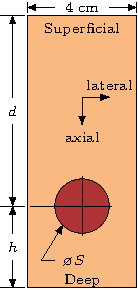
\includegraphics[width=0.9375in]{assets/quasistatic/drawings/schematic_single-crop.pdf}
				\label{fig:schematic_single}
			}
			~
			\subfloat[]{
				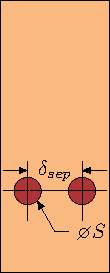
\includegraphics[width=0.7623625in]{assets/quasistatic/drawings/schematic_colocated-crop.pdf}
				\label{fig:schematic_colocated}
			}
			~
			\subfloat[]{
				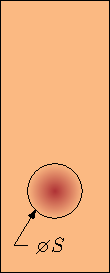
\includegraphics[width=0.7623625in]{assets/quasistatic/drawings/schematic_blur-crop.pdf}
				\label{fig:schematic_blur}
			}
			~
			\subfloat[]{
				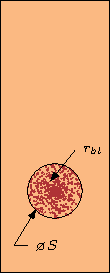
\includegraphics[width=0.7623625in]{assets/quasistatic/drawings/schematic_blob-crop.pdf}
				\label{fig:schematic_blob}
			}
			~
			\subfloat[]{
				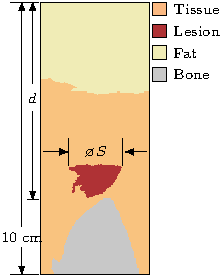
\includegraphics[width=1.4938125in]{assets/quasistatic/drawings/schematic_human-crop.pdf}
				\label{fig:schematic_human}
			}
			\caption[Quasi-static model geometries]{Model geometry showing the investigated lesions embedded in a \SI{4}{\cm} wide soft tissue domain. Axial and lateral directions mimic that of a typical ultrasound transducer placed along the top boundary of the domain. The simplest case of a circular lesion embedded in a soft tissue domain located superior to hard underlying bone is shown in \protect\subref{fig:schematic_single}. In order to investigate the interference caused by closely-located lesions, the case shown in \protect\subref{fig:schematic_colocated} was investigated. Because of the relatively unknown and variable geometric properties of deep tissue injury lesions, cases \protect\subref{fig:schematic_blur} and \protect\subref{fig:schematic_blob} were investigated where the lesion edges were blurred and the lesion was actually a large collection of small lesions, respectively. Finally, to investigate detection sensitivity in a realistic setting, case \protect\subref{fig:schematic_human} was investigated where an mri-acquired deep tissue injury was overlaid on a slice from the Visible Human Project such that the injury lesion was located immediately superior to an ischial tuberosity.}	
			\label{fig:geometry}
		\end{figure*}

		Simulated ultrasound images were acquired through the convolution of a point spread function with a normally distributed background map of scattering centres \cite{bamber80}. These images were then combined with a finite-element deformation model of the strained tissue to generate both pre- and post- compression images of the lesions and surrounding tissue. These images were fed into a tissue strain estimation algorithm to determine the detection sensitivity of the technique. Finally, the technique was validated against a physical phantom model using a subset of the simulated cases.

		\subsection{Formation of B-Mode Ultrasound Images}
			Through the convolution of a point spread function and a normal random distribution of scattering centres, simulated ultrasound images were generated. The point spread function was defined axially as a cosine function operating at the ultrasound probing frequency modulated by a Gaussian distribution defined by $\mu = 2\lambda$ and $\sigma = 2\lambda$ where $\lambda$ is the wavelength of the ultrasonic probing waves. Laterally, the point spread function was modelled as a Gaussian distribution defined by $\mu = 0$ and $\sigma = 0.25w_{active}$ where $w_{active}$ is the total width of the active transducer elements during scan-line acquisition.  This resulted in the point spread function given in Fig. \ref{fig:point_spread_function}. Resulting images were composed of 192 scan lines each sampled at \SI{50}{\MHz}.

			\begin{figure}[!htb]
				\centering
					\begin{tikzpicture}
						\begin{axis}[
						width=0.75\textwidth,
						enlargelimits=false,
						unit vector ratio*=1 1 1,
						axis on top,
						xlabel={Lateral (\si{\mm})},
						ylabel={Axial (\si{\mm})},
						y dir=reverse,
						draw=black, text=black, fill=black
						]
							\addplot graphics[xmin=-1.15,xmax=1.15,ymin=0,ymax=1.54]{assets/quasistatic/images/psf.png};
						\end{axis}
					\end{tikzpicture}
				\caption[Point spread function used for simulating b-mode ultrasound scans]{Point spread function used for simulating b-mode ultrasound scans. The function is defined axially by a cosine function at the probing frequency and modulated by a Gaussian function both axially and laterally.}
				\label{fig:point_spread_function}
			\end{figure}

		\subsection{Finite-Element Model of Tissue Deformation Under Surface Distortion}
			As a response to an external load being applied to the boundary of a domain, internal structures deform. In the case of a relatively stiff deep tissue injury embedded within surrounding soft tissues, this implies that when the surface of the skin is depressed, the relatively stiff lesion will not strain to the same magnitude that the surrounding soft tissue does. In order to simulate the deformation of interrogated tissue, the displacement field for the simulated models was calculated according to:
			\begin{equation}
				- {\nabla} \cdot \sigma = {F}
			\end{equation}
			Where $\sigma$ is the Cauchy stress tensor and $F$ are the applied body forces. Simulations were performed assuming a 2-dimensional linearly elastic material deformation model under plane strain conditions. A 3-dimensional model was also considered, however the deformations differed from the 2-dimensional simulation by less than \SI{1}{\percent} so a 2-dimensional model was deemed adequate. Soft tissue was modelled using a Young's modulus of elasticity of \SI{25}{\kPa}, Poisson's ratio of 0.499, and density of \SI{998}{\kg\per\metre\cubed} \cite{krouskop98, choi05, martin94}. Bone was modelled in the Visible Human model with a Young's modulus of elasticity of \SI{18.6}{\GPa}, Poisson's ratio of 0.15 and density of \SI{297}{\kg\per\metre\cubed} \cite{rho93,shahar07,zheng00}. The only difference in lesion mechanical properties from the surrounding soft tissue was the modulus of elasticity which varied according to the simulation parameters. The bottom of the domain was held fixed such that:
			\begin{equation}
				{u} = 0, \qquad \Gamma = \Gamma_{bottom}
			\end{equation}
			While this boundary condition represents an idealized scenario, it may be likened to that of tissue located superficial to a relatively stiff anchoring bone below since the stiffness of bone is several orders of magnitude greater than soft tissue and will not significantly deform under the loads explored in this model. This lower region is where deep tissue injuries generally form and is therefore of special importance. Compressive strains were applied to the top of the domain so as to induce strain along the top boundary:
			\begin{equation}
				{u} = (0, -u_0), \qquad \Gamma = \Gamma_{top}
			\end{equation}

			From these simulations, displacement fields throughout the domain were calculated which were then used to displace tissue (including scattering centres) in the simulated ultrasound images in both the axial and lateral directions. This process resulted in pairs of pre- and post- compression simulated b-mode images of lesions of varying parameters which could then be analyzed and characterized.

		\subsection{Characterizing Quasi-Static Ultrasound Elastography}
			\label{sec:elastography_algorithm}
			Utilizing a 2-D locally regularized tissue strain estimation algorithm \cite{brusseau08}, pairs of pre- and post- compression images were used to calculate elastogram estimations for the full range of parameter values of the simulated lesions. The algorithm consists of sweeping the image domain with a series of overlapping regions of interest (ROI). ROI are compared between pre- and post- compression images, with ROI in the post- compression images being axially scaled and translated and laterally translated versions of the same ROI in the pre-compression images.

			Qualitatively, the noise and computation time of the resulting elastograms were found to be minimum when using an axial ROI size of approximately 10 times the ultrasound wavelength. Axial ROI overlap was held at \SI{99}{\percent} to produce elastograms with minimal noise, even though this introduced significant increases in computation time. Due to the extreme anisotropic nature of ultrasound signals, lateral ROI size was kept to 5 signal widths with lateral ROI overlaps of \SI{80}{\percent}.

		\subsection{Model Validation Using a Commercially Available Phantom}
			Utilizing a CIRS Elasticity QA Phantom model 049, a subset of the results obtained from the finite-element simulations and numerical characterizations were compared against their physical phantom equivalents. The phantom mimics acoustically homogeneous soft tissue with embedded lesions which vary in depth, size, and mechanical stiffness. Mechanical properties of the phantom as given by manufacturer specifications are summarized in Table \ref{tab:phantomproperties}. Pre- and post- compression b-mode ultrasound images were obtained of each lesion in the phantom and the resulting strain ratio for that lesion was compared to the simulated strain ratio for that combination of parameters. Specifically, lesions at a depth of \SI{3.5}{\cm}, a diameter of \SI{2.0}{\cm}, and with true stiffness ratios of 0.56, 1.80, and 3.20 were examined. Surface indentation was performed manually with the transducer indenting approximately \SI{0.5}{\cm} (\SI{6.25}{\percent}) at the surface.

			\begin{table}[!htb]
				\centering
				\caption{CIRS Phantom Model Mechanical Properties}
				\label{tab:phantomproperties}
				\begin{tabular}{lr}
					\toprule
					Property & Value \\
					\midrule
					Nominal basal stiffness & \SI{25}{\kPa} \\
					Lesion stiffness &  $[8, 14, 45, 80]$\,\si{\kPa} \\
					Speed of sound & \SI{1540}{\metre\per\second} \\
					Acoustic attenuation & \SI{0.5}{\decibel\per\cm\per\MHz} \\
					Lesion diameter & $[10, 20]$\,\si{\mm} \\
					Lesion depth & $[15, 35]$\,\si{\mm} \\
					\bottomrule
				\end{tabular}
			\end{table}

	\section{Results and Discussion}
		Following the procedure outlined in Section \ref{sec:method}, finite-element models of ultrasonic b-mode image formation and tissue deformation were synthesized. The results of these models were then fed into the local strain estimation algorithm described in Section \ref{sec:elastography_algorithm}. The resulting numerical characterizations of the relationship between measured and true strain ratios in the simulated tissue and their dependence on the various lesion parameters given in Table \ref{tab:quasi-parametervalues} were examined. Finally, the local strain estimation algorithm was carried out on a physical phantom and compared against a subset of the simulated cases.

		\subsection{Finite Element Models of Ultrasound and Deformation}
			\label{sec:femresults}
			Sample images generated using both the acoustic and deformation finite-element models are given in Figs. \ref{fig:precompression_bmode} -- \ref{fig:postcompression_bmode}. In Fig. \ref{fig:precompression_bmode}, a sample generated b-mode ultrasound scan is given. Fig. \ref{fig:displacement_field_u} shows the lateral displacement field generated by the deformation finite-element model while Fig. \ref{fig:displacement_field_v} shows the axial displacement field. The entire top surface of the model has been displaced axially by \SI{6.25}{\mm} (\SI{5}{\percent}), which caused deformation of both the soft tissue and embedded lesion within. Since the lesion was modelled as being 3.2 times stiffer than the surrounding tissue, the lesion underwent less strain which consequently resulted in the lesser displacement depicted. Fig. \ref{fig:postcompression_bmode} shows the resultant b-mode image generated by applying the displacement field given in Figs. \ref{fig:displacement_field_u} and \ref{fig:displacement_field_v} to the tissue and embedded scattering centres used to create Fig. \ref{fig:precompression_bmode}. What results is a locally scaled and translated version of Fig. \ref{fig:precompression_bmode} that corresponds to indenting the surface of the skin above a stiff lesion. The large anechoic region located at the bottom of the domain is tissue that was not modelled in the pre-compression image as it was outside of the original domain. This area represents the region of tissue that is undetectable with the strain-estimation algorithm given in Section \ref{sec:elastography_algorithm} as the information contained there is only available in one of the two input images and so is considered incomplete data.

			\addtocounter{footnote}{-1}
			\begin{figure*}[!htb]
				\centering
				\subfloat[]{
					\begin{tikzpicture}
						\begin{axis}[width=0.65\textwidth, enlargelimits=false, unit vector ratio*=1 1 1, axis on top, xlabel={Lateral deviation, $x$ (\si{\cm})}, ylabel={}, y dir=reverse, colormap name={RdBu}, colorbar, point meta min=-1.17, point meta max=1.17, colorbar style={at={(1.05,0)}, anchor=south west, width=0.01\textwidth, ylabel={Lateral Displacement (\si{\mm})},
						draw=black, text=black, fill=black},
						draw=black, text=black, fill=black]
							\addplot graphics[xmin=-2,xmax=2,ymin=0,ymax=12.5]{assets/quasistatic/images/displacement_u_colour.png};
						\end{axis}
					\end{tikzpicture}
					\label{fig:displacement_field_u}
				}
				~
				\subfloat[]{
					\begin{tikzpicture}
						\begin{axis}[width=0.65\textwidth, enlargelimits=false, unit vector ratio*=1 1 1, axis on top, xlabel={Lateral deviation, $x$ (\si{\cm})}, ylabel={}, y dir=reverse, colormap name={YlOrRd}, colorbar, point meta min=-6.25, point meta max=0, colorbar style={at={(1.05,0)}, anchor=south west, width=0.01\textwidth, ylabel={Axial Displacement (\si{\mm})},
						draw=black, text=black, fill=black, y dir=reverse},
						draw=black, text=black, fill=black]
							\addplot graphics[xmin=-2,xmax=2,ymin=0,ymax=12.5]{assets/quasistatic/images/displacement_v_colour.png};
						\end{axis}
					\end{tikzpicture}
					\label{fig:displacement_field_v}
				}
				
				\subfloat[]{
					\begin{tikzpicture}
						\begin{axis}[width=0.65\textwidth, enlargelimits=false, unit vector ratio*=1 1 1, axis on top, xlabel={Lateral deviation, $x$ (\si{\cm})}, ylabel={Depth, $d$ (\si{\cm})}, y dir=reverse,
						draw=black, text=black, fill=black]
							\addplot graphics[xmin=-2,xmax=2,ymin=0,ymax=12.5]{assets/quasistatic/images/bModeA.png};
						\end{axis}
					\end{tikzpicture}
					\label{fig:precompression_bmode}
				}
				~
				\subfloat[]{
					\begin{tikzpicture}
						\begin{axis}[width=0.65\textwidth, enlargelimits=false, unit vector ratio*=1 1 1, axis on top, xlabel={Lateral deviation, $x$ (\si{\cm})}, ylabel={Depth, $d$ (\si{\cm})}, y dir=reverse,
						draw=black, text=black, fill=black]
							\addplot graphics[xmin=-2,xmax=2,ymin=0,ymax=12.5]{assets/quasistatic/images/bModeB.png};
						\end{axis}
					\end{tikzpicture}
					\label{fig:postcompression_bmode}
				}
				\caption[Sample deformation finite-element model results for a hard spherical lesion]{Finite-element model results for the case when \ensuremath{d=\SI{10}{\cm}}, \ensuremath{\diameter S = \SI{2.5}{\cm}}, \ensuremath{\varepsilon_{rel} = 3.20}, and \ensuremath{f=\SI{4}{\MHz}} showing \protect\subref{fig:displacement_field_u} the lateral displacement field and \protect\subref{fig:displacement_field_v} the axial displacement field induced by compressive strain applied to the top of the boundary, \protect\subref{fig:precompression_bmode} a generated b-mode image of the pre-compressed tissue domain, and \protect\subref{fig:postcompression_bmode} a generated b-mode image of the post-compressed tissue domain. The included lesion is not visible in \protect\subref{fig:precompression_bmode} and \protect\subref{fig:postcompression_bmode} as it's acoustic properties were no different than surrounding tissues. An anechoic region is visible along the bottom of the domain in \protect\subref{fig:postcompression_bmode} which represents tissue outside of the domain visible in \protect\subref{fig:precompression_bmode}.}
				\label{fig:modelresults}
			\end{figure*}

		\FloatBarrier
		\subsection{Resulting Elastograms}
			\label{sec:elastogram}
			The 2-D locally regularized tissue strain estimation algorithm described in Section \ref{sec:elastography_algorithm} was used in combination with the simulated resultant b-mode ultrasound images (Figs. \ref{fig:precompression_bmode} and \ref{fig:postcompression_bmode}) in order to generate elastogram images which were used in the subsequent analysis. An example elastogram resulting from the simulation presented in Fig. \ref{fig:modelresults} is shown in Fig. \ref{fig:sample_elastogram}. Throughout the entire domain on this sample elastogram, regions outside of the stiff lesions showed compressive strains of approximately \SI{5}{\percent} as expected due to the compression applied to the upper boundary of the model. The entire lesion region showed relatively consistent low strain amounts of approximately \SI{2.5}{\percent}, which is consistent with the lesion being stiffer (and so straining less) than the surrounding tissue. Of note is the increased strain pattern which appeared both axially and laterally around the lesion. While generally symmetric about the axial direction, this stress field was largely concentrated above the lesion when the lesion was deep (close to the bone). This may be explained as a stress concentration brought about by the sudden change in mechanical material properties of the tissue and may serve to fuel the conditions of excessive cell deformation and ischemia which initiated the formation of a deep tissue injury in the first place, exacerbating the wound and assisting its expansion toward the surface. Further, a largely variable strain field artifact is seen along the superior surface of the elastogram shown in Fig. \ref{fig:sample_elastogram}. While this field does not appear to affect the remainder of the generated elastogram, it will serve to mask any extremely shallow legions in the tissue, though given as deep tissue injuries generally form immediately superior to boney prominences, this is unlikely to be the case. It is hypothesized that this variable strain field may be due to the large deformations present along the superior surface of the domain.

			\begin{figure}[!htb]
				\centering
					\begin{tikzpicture}
						\begin{axis}[width=\columnwidth, enlargelimits=false, unit vector ratio*=1 1 1, axis on top, xlabel={Lateral deviation, $x$ (\si{\cm})}, ylabel={Depth, $d$ (\si{\cm})}, y dir=reverse, colormap name={YlOrRd}, colorbar, point meta min=0, point meta max=7, colorbar style={yticklabel={\pgfmathprintnumber{\tick}\,\percent},at={(1.05,0)}, width=0.01\textwidth, ylabel={Compressive Strain}, anchor=south west,
						draw=black, text=black, fill=black},
						draw=black, text=black, fill=black]
							\addplot graphics[xmin=-2,xmax=2,ymin=0,ymax=12.5]{assets/quasistatic/elastograms/e040_colour.png};
						\end{axis}
					\end{tikzpicture}
				\caption[Sample strain elastogram for a hard spherical lesion]{Sample strain elastogram showing estimated strain values for $d=\SI{10}{\cm}$, $\diameter S = \SI{2.5}{\cm}$, $\varepsilon_{rel} = 3.20$, $f = \SI{4}{\MHz}$. While undetectable on a single b-mode image, the elastogram clearly shows a low-strain (stiff) lesion located approximately \SI{10}{\cm} from the surface.}
				\label{fig:sample_elastogram}
			\end{figure}

		\subsection{Numerical Characterizations}
			\label{sec:numericalcharacterizations}
			In order to determine the sensitivity of using quasi-static ultrasound elastography to detect deep tissue injuries, elastograms such as the example that was calculated in Section \ref{sec:elastogram} were calculated for the full range of parameters given in Table \ref{tab:quasi-parametervalues}. ``Measured'' strain ratios for each elastogram were obtained by comparing the mean strain within each lesion with the mean engineering strain of the surrounding tissue such that:
			\begin{equation}
				\varepsilon_{rel,measured} = \frac{\varepsilon_{tissue}}{\varepsilon_{lesion}}
			\end{equation}

			$\varepsilon_{tissue}$ was sampled as the mean strain in the region of tissue with the same geometry as the lesion located immediately superficial to the lesion in all cases.

			In order to characterize how each parameter of interest affects the detection sensitivity of quasi-static ultrasound elastography, measured strain ratios for various lesions were calculated and compared against $\varepsilon_{rel,true}$. $\varepsilon_{rel,true}$ is derived from the relative Young's modulus of elasticity of the lesion such that:
			\begin{equation}
				\varepsilon_{rel,true} = \frac{\varepsilon_{tissue}}{\varepsilon_{lesion}} = \frac{\left(\frac{\sigma_{applied}}{E_{tissue}}\right)}{\left(\frac{\sigma_{applied}}{E_{lesion}}\right)} = \frac{E_{lesion}}{E_{tissue}}
			\end{equation}

			\begin{figure}[!htb]
				\centering
				\begin{tikzpicture}
					\begin{axis}[
						scale only axis,
						height=3in,
						width=\textwidth-\widthof{100}-1in,
						xlabel={Lesion Stiffness Ratio},
						ylabel={\percent\ Error},
						grid=major,
						clip=true,
						cycle list name=ColourPlotCycle,
						draw=black, text=black, fill=black]
						\addplot+[error bars/.cd, y dir=both, y explicit, error bar style={ultra thick}] table[x index=0, y index=1, y error index=2] {assets/quasistatic/data/error_stiffness_ratio.dat};
					\end{axis}
				\end{tikzpicture}
				\caption[Detection ability as it is related to true lesion stiffness ratio]{Detection ability as it is related to true lesion stiffness ratio. For all but small lesion stiffness ratios (very soft ``lesions''), results are linear and predictable. For small lesion stiffness ratios (0.32), the lesion becomes severely misrepresented. This is likely due to the algorithm ``losing track'' of scattering centres for the relatively large displacements induced in the significantly less stiff tissue.}
				\label{fig:error_stiffness_ratio}
			\end{figure}

			Fig. \ref{fig:error_stiffness_ratio} portrays the severe error involved with using the methods described in Section \ref{sec:method} to investigate extremely low stiffness lesions. In nearly all investigated cases where the true lesion stiffness ratio was 0.32, the algorithms described severely misrepresented the measured strain ratio of the lesion, often portraying these extremely low stiffness regions as being more stiff than they truly were. It is hypothesized that the excessively large localized deformations in these lesions interrupted the algorithm's ability to sufficiently track the displacement of scattering centres within the tissue, lowering the magnitude of displacement within the lesion and subsequently increasing it's ``measured'' strain ratio.

			\begin{figure}[!htb]
				\centering
				\begin{tikzpicture}
					\begin{axis}[
						scale only axis,
						height=3in,
						width=\textwidth-\widthof{100}-1in,
						xlabel={Normalized Characterization Index},
						ylabel={\percent\ Error},
						grid=major,
						legend entries={Lesion Size, Lesion Depth, Bone Separation, Probing Frequency, Applied Strain},
						legend style={at={(0.5,0.975)},anchor=north,font=\small},
						clip=true,
						cycle list name=ColourPlotCycle,
						ymax=70,
						draw=black, text=black, fill=black]
						\addplot table {assets/quasistatic/data/normalized_size.dat};
						\addplot table {assets/quasistatic/data/normalized_depth.dat};
						\addplot table {assets/quasistatic/data/normalized_bottomsep.dat};
						\addplot table {assets/quasistatic/data/normalized_frequency.dat};
						\addplot table {assets/quasistatic/data/normalized_strain.dat};
					\end{axis}
				\end{tikzpicture}
				\caption[Error characterization for a hard spherical lesion]{Error characterization for range of studied parameters for the simple model of a spherical lesion embedded within soft tissue as seen in Fig. \ref{fig:schematic_single}. Each parameter has been normalized to the range studied so overly-sensitive regions may be readily distinguished.}
				\label{fig:normalized_characterization}
			\end{figure}

			\begin{figure}[!htb]
				\centering
				\begin{tikzpicture}
					\begin{axis}[
						scale only axis,
						height=3in,
						width=\textwidth-\widthof{100}-1in,
						xlabel={Normalized Characterization Index},
						ylabel={\percent\ Error},
						grid=major,
						legend entries={Boundary Blur Radius, Co-Located Lesion Separation, Clustered Lesion Density, Clustered Lesion Size, Human Lesion Size, Human Lesion Depth},
						legend style={legend pos=north east,font=\small},
						clip=true,
						cycle list name=ColourPlotCycle,
						ymax=80,
						draw=black, text=black, fill=black]
						\addplot table {assets/quasistatic/data/normalized_lesion_sep.dat};
						\addplot table {assets/quasistatic/data/normalized_blur_radius.dat};
						\addplot table {assets/quasistatic/data/normalized_blob_density.dat};
						\addplot table {assets/quasistatic/data/normalized_blob_radius.dat};
						\addplot table {assets/quasistatic/data/normalized_human_size.dat};
						\addplot table {assets/quasistatic/data/normalized_human_depth.dat};
					\end{axis}
				\end{tikzpicture}
				\caption[Error characterization for: co-located, blurred boundary, clustered, and visible human lesion models]{Error characterization for range of studied parameters for the co-located lesions, blurred boundary lesions, clustered lesions, and visible human lesion models as seen in Figs. \ref{fig:schematic_colocated} -- \ref{fig:schematic_human}. Each parameter has been normalized to the range studied so overly-sensitive regions may be readily distinguished.}
				\label{fig:normalized_characterization_extras}
			\end{figure}

			In order to broadly investigate the critical parameter-values of the investigated models, each parameter was normalized to its investigated range and the error resulting over these ranges is given in Figs. \ref{fig:normalized_characterization} and \ref{fig:normalized_characterization_extras}.

			In Fig. \ref{fig:normalized_characterization}, it is clear to see that the most sensitive error-inducing situations occur when either the lesion is very small or if large strains are used to deform the tissue. Similarly, it is expected that if the lesion depth were increased much further, significant errors would arise with increasing depth. Logically, this may be explained due to the decreasing magnitude of displacement with increasing depth---at a certain point, the magnitude of displacement of scattering centres will be on par with the measurement noise, and the lesion will cease to be detectable.

			From Fig. \ref{fig:normalized_characterization_extras} it can be seen that small lesions in the Visible Human-MRI model as well as co-located lesions with large separation distances produce greater measurement errors. Conversely, lesion depth in the Visible Human-MRI model; lesion density and individual lesion size in the clustered lesion model; and boundary blur radius in the blurred-edges model do not seem to affect the measurement error significantly. Of note is the relative large amount of static error present in the boundary blur radius model which is hypothesized to be due to lesser mean tissue stiffness in the investigated region than expected.

			\begin{figure}[!htb]
				\centering
				\begin{tikzpicture}
					\begin{axis}[
						scale only axis,
						height=3in,
						width=\textwidth-\widthof{100}-1in,
						xlabel={True Lesion Stiffness Ratio, $E_{true}$},
						ylabel={Measured Lesion Stiffness Ratio, $E_{meas}$},
						grid=major,
						legend entries={$\diameter S = \SI{0.5}{\cm}$, $\diameter S = \SI{1.0}{\cm}$, $\diameter S = \SI{2.0}{\cm}$, $\diameter S = \SI{2.5}{\cm}$},
						legend style={legend pos=north west,font=\small},
						clip=true,
						cycle list name=ColourPlotCycle,
						draw=black, text=black, fill=black]
						\addplot table {assets/quasistatic/data/circular_size_05.dat};
						\addplot table {assets/quasistatic/data/circular_size_10.dat};
						\addplot table {assets/quasistatic/data/circular_size_20.dat};
						\addplot table {assets/quasistatic/data/circular_size_25.dat};
						\node [anchor=south](c) at (axis cs:3.125,0.6) {
\includegraphics{assets/quasistatic/insets/inset_single.pdf}};
					\end{axis}
				\end{tikzpicture}
				\caption[Quasi-static lesion size characterization]{Lesion size characterization at a depth of \SI{10}{\cm} with a \SI{4}{\MHz} ultrasound probing frequency showing increasing detection sensitivity of the lesion with increasing lesion size. Detection sensitivity is less than ideal for all cases, with the best case being for lesions approximately \SI{2.5}{\cm} in diameter.}
				\label{fig:size_characterization}
			\end{figure}

			Fig. \ref{fig:size_characterization} shows the relationship between lesion size and detection sensitivity for lesions at a depth of \SI{10}{\cm} in a model depth of \SI{12.5}{\cm} interrogated at \SI{4}{\MHz} with \SI{5}{\percent} applied strain. Specifically, Fig. \ref{fig:size_characterization} shows the decreasing detection sensitivity with decreasing lesion size with the best detection sensitivity being with the largest investigated lesions with a diameter of \SI{2.5}{\cm}. On the opposite end, the detection sensitivity of lesions at or below \SI{0.5}{\cm} in diameter is questionable. Although data is lacking on the true size of formative DTI, MRI results indicate that untreated DTI are on the scale of multiple centimetres \cite{solis13}. Thus, the ability to detect lesions of at least \SI{1}{\cm} in diameter should prove to be adequate to both detect and monitor DTI.

			In order to investigate the effect of lesion depth on the detection sensitivity, measured strain ratios for circular lesions with a diameter of \SI{2.5}{\cm} located at various depths were interrogated with a \SI{4}{\MHz} probing frequency, and strained by \SI{5}{\percent}. The results of this investigation are seen in Fig. \ref{fig:depth_characterization}.

			\begin{figure}[!htb]
				\centering
				\begin{tikzpicture}
					\begin{axis}[
						scale only axis,
						height=3in,
						width=\textwidth-\widthof{100}-1in,
						xlabel={True Lesion Stiffness Ratio, $E_{true}$},
						ylabel={Measured Lesion Stiffness Ratio, $E_{meas}$},
						grid=major,
						legend entries={$d = \SI{3.5}{\cm}$, $d = \SI{6.5}{\cm}$, $d = \SI{8.5}{\cm}$, $d = \SI{10}{\cm}$},
						legend style={legend pos=north west,font=\small},
						clip=true,
						cycle list name=ColourPlotCycle,
						draw=black, text=black, fill=black]
						\addplot table {assets/quasistatic/data/circular_depth_035.dat};
						\addplot table {assets/quasistatic/data/circular_depth_065.dat};
						\addplot table {assets/quasistatic/data/circular_depth_085.dat};
						\addplot table {assets/quasistatic/data/circular_depth_100.dat};
						\node [anchor=south](c) at (axis cs:3.125,0.6) {
\includegraphics{assets/quasistatic/insets/inset_single.pdf}};
					\end{axis}
				\end{tikzpicture}
				\caption[Quasi-static lesion depth characterization]{Lesion depth characterization at a lesion diameter of \SI{2.5}{\cm} with a \SI{4}{\MHz} ultrasound probing frequency generally showing general independence of detection sensitivity on lesion depth in the tissue.}
				\label{fig:depth_characterization}
			\end{figure}

			In Fig. \ref{fig:depth_characterization}, it can be seen that there was little interplay between detection sensitivity and measured strain ratios at the various depths examined for all but the case for very soft (mushy) lesions (with a stiffness ratio of 0.32). At such low stiffness ratios, the excessive tissue deformation interrupts the tissue strain estimation algorithm's ability to adequately track the induced displacements in the lesion.

			Since the strain field caused by compressive forces near an extremely rigid structure embedded within a relatively soft domain will be significantly heterogeneous, the effect of lesion altitude above the underlying stiff bone was examined with the hypothesis that if the lesion were too close to the hard bone, it would be masked by the strain field caused by the bone's existence. A \SI{2.5}{\cm} diameter lesion was interrogated with a \SI{4}{\MHz} probing frequency and \SI{5}{\percent} applied strain. The results of this characterization are given in Fig. \ref{fig:bottomsep_characterization}.

			\begin{figure}[!htb]
				\centering
				\begin{tikzpicture}
					\begin{axis}[
						scale only axis,
						height=3in,
						width=\textwidth-\widthof{100}-1in,
						xlabel={True Lesion Stiffness Ratio, $E_{true}$},
						ylabel={Measured Lesion Stiffness Ratio, $E_{meas}$},
						grid=major,
						legend entries={$h = \SI{1.25}{\cm}$, $h = \SI{2.50}{\cm}$, $h = \SI{3.75}{\cm}$},
						legend style={legend pos=north west,font=\small},
						clip=true,
						cycle list name=ColourPlotCycle,
						draw=black, text=black, fill=black]
						\addplot table {assets/quasistatic/data/circular_bottomsep_000.dat};
						\addplot table {assets/quasistatic/data/circular_bottomsep_125.dat};
						\addplot table {assets/quasistatic/data/circular_bottomsep_250.dat};
						\node [anchor=south](c) at (axis cs:3.125,0.6) {
\includegraphics{assets/quasistatic/insets/inset_single.pdf}};
					\end{axis}
				\end{tikzpicture}
				\caption[Quasi-static lesion altitude characterization]{Effect of lesion altitude above the underlying bone. Aside from erroneous results at very low lesion stiffness ratios, the effect is negligible.}
				\label{fig:bottomsep_characterization}
			\end{figure}

			In Fig. \ref{fig:bottomsep_characterization}, it can be seen that the lesion altitude above the underlying bone had very little effect on the detection sensitivity. Although larger strain fields may be generated near the bone, it is hypothesized that the larger fields also extend larger and so affect healthy tissue to more or less the same degree as the forming lesion.

			In order to characterize the effect of using alternate ultrasound probing frequencies, simulations were carried out on lesions using probing frequencies of \SI{2}{\MHz}, \SI{4}{\MHz}, and \SI{8}{\MHz}. The simulated lesions had a diameter of \SI{2.5}{\cm}, were located at a depth of \SI{10}{\cm} and we strain at \SI{5}{\percent}. The results of this study are given in Fig. \ref{fig:freq_characterization}.

			\begin{figure}[!htb]
				\centering
				\begin{tikzpicture}
					\begin{axis}[
						scale only axis,
						height=3in,
						width=\textwidth-\widthof{100}-1in,
						xlabel={True Lesion Stiffness Ratio, $E_{true}$},
						ylabel={Measured Lesion Stiffness Ratio, $E_{meas}$},
						grid=major,
						legend entries={$f = \SI{2}{\MHz}$, $f = \SI{4}{\MHz}$, $f = \SI{8}{\MHz}$},
						legend style={legend pos=north west,font=\small},
						clip=true,
						cycle list name=ColourPlotCycle,
						draw=black, text=black, fill=black]
						\addplot table {assets/quasistatic/data/circular_frequency_2.dat};
						\addplot table {assets/quasistatic/data/circular_frequency_4.dat};
						\addplot table {assets/quasistatic/data/circular_frequency_8.dat};
						\node [anchor=south](c) at (axis cs:3.125,0.55) {
\includegraphics{assets/quasistatic/insets/inset_single.pdf}};
					\end{axis}
				\end{tikzpicture}
				\caption[Quasi-static ultrasound probing frequency characterization]{Characterization of ultrasonic probing frequency on detection sensitivity. Apart from the requirement of using an ultrasonic frequency low enough to interrogate the desired tissue, probing frequency has negligible effect on the detection sensitivity.}
				\label{fig:freq_characterization}
			\end{figure}

			As can be seen from Fig. \ref{fig:freq_characterization}, there is very little effect on the detection sensitivity from the ultrasound probing frequency that was used, therefore an appropriate frequency should be chosen so as to reach the the full depth of the bone-muscle interface at suspected DTI locations while retaining the best image resolution.

			As quasi-static ultrasound elastography is most likely to be performed via manual indentation where the exact magnitude of applied deformation is unknown, it is important to study the effect of applied strain magnitude on the detection sensitivity. Applied strains of \SI{2.5}{\percent}, \SI{5.0}{\percent}, and \SI{10}{\percent} were investigated on a \SI{2.5}{\cm} diameter lesion at a depth of \SI{10}{\cm} using a probing frequency of \SI{4}{\MHz}; the results are given in Fig. \ref{fig:strain_characterization}.

			\begin{figure}[!htb]
				\centering
				\begin{tikzpicture}
					\begin{axis}[
						scale only axis,
						height=3in,
						width=\textwidth-\widthof{100}-1in,
						xlabel={True Lesion Stiffness Ratio, $E_{true}$},
						ylabel={Measured Lesion Stiffness Ratio, $E_{meas}$},
						grid=major,
						legend entries={$\varepsilon_{app} = \SI{2.5}{\percent}$, $\varepsilon_{app} = \SI{5.0}{\percent}$, $\varepsilon_{app} = \SI{10.0}{\percent}$},
						legend style={legend pos=north west,font=\small},
						clip=true,
						cycle list name=ColourPlotCycle,
						draw=black, text=black, fill=black]
						\addplot table {assets/quasistatic/data/circular_strain_025.dat};
						\addplot table {assets/quasistatic/data/circular_strain_050.dat};
						\addplot table {assets/quasistatic/data/circular_strain_100.dat};
						\node [anchor=south](c) at (axis cs:3.125,0.6) {
\includegraphics{assets/quasistatic/insets/inset_single.pdf}};
					\end{axis}
				\end{tikzpicture}
				\caption[Quasi-static applied strain characterization]{Applied strain characterization plot for lesions with a diamater of \SI{2.5}{\cm} located at a depth of \SI{10}{\cm} interrogated at \SI{4}{\MHz}. There is little difference between \SI{2.5}{\percent} and \SI{5.0}{\percent} applied strain, while large-magnitude strains of \SI{10}{\percent} generate significant error for both very soft and very stiff lesions.}
				\label{fig:strain_characterization}
			\end{figure}

			While Fig. \ref{fig:strain_characterization} shows a relatively constant detection sensitivity for compressive strains of \SI{2.5}{\percent} and \SI{5}{\percent}, compressive strains of \SI{10}{\percent} generate significant measurement error for both very soft and very stiff lesions. Under large compressive strains, the tissue (either in the lesion as in the soft lesion case, or the surrounding tissue as in the stiff lesion case) deforms considerably which again interferes with the algorithm's ability to properly track the displacement of tissue. It should also be noted that applying overly large strains to an already forming deep tissue injury may cause additional unwarranted damage. Thus it is imperative that applied surface indentation be kept to reasonable bounds (\SI{2.5}{\percent} -- \SI{5}{\percent}, or \SI{0.25}{\cm} -- \SI{0.50}{\cm} in \SI{10}{\cm} deep domains), not only for safety of the tissue but also for clarity of the diagnostic test.

			To study the effect that closely spaced lesions will have on the detection sensitivity as well as how discernible the lesions will be from each other, the separation distance between two \SI{1.0}{\cm} diameter co-located lesions at a depth of \SI{10}{\cm} was examined using a \SI{4}{\MHz} probing frequency with \SI{5}{\percent} applied strain magnitude. The results of this study are shown in \ref{fig:separation_characterization}.

			\begin{figure}[!htb]
				\centering
				\begin{tikzpicture}
					\begin{axis}[
						scale only axis,
						height=3in,
						width=\textwidth-\widthof{100}-1in,
						xlabel={True Lesion Stiffness Ratio, $E_{true}$},
						ylabel={Measured Lesion Stiffness Ratio, $E_{meas}$},
						grid=major,
						legend entries={$\delta_{sep} = \SI{1.25}{\cm}$, $\delta_{sep} = \SI{1.50}{\cm}$, $\delta_{sep} = \SI{1.75}{\cm}$, $\delta_{sep} = \SI{2.00}{\cm}$},
						legend style={legend pos=north west,font=\small},
						clip=true,
						cycle list name=ColourPlotCycle,
						draw=black, text=black, fill=black]
							\addplot table {assets/quasistatic/data/separation_0125.dat};
							\addplot table {assets/quasistatic/data/separation_0150.dat};
							\addplot table {assets/quasistatic/data/separation_0175.dat};
							\addplot table {assets/quasistatic/data/separation_0200.dat};
							\node [anchor=south](c) at (axis cs:3.125,0.7) {
\includegraphics{assets/quasistatic/insets/inset_colocated.pdf}};
					\end{axis}
				\end{tikzpicture}
				\caption[Quasi-static lesion separation distance characterization]{Effect of lesion separation distance on two \SI{1.0}{\cm} diameter lesions co-located at a depth of \SI{10}{\cm} interrogated with a \SI{4}{\MHz} probe with \SI{5}{\percent} applied strain. There is no negligible difference between separation distances on the detection sensitivity.}
				\label{fig:separation_characterization}
			\end{figure}

			While Fig. \ref{fig:separation_characterization} shows that the separation distance between co-located lesions causes a negligible effect on the detection sensitivity, Fig. \ref{fig:separation_elastogram} shows regions of decreased strain above and below the centreline of the lesions. While these regions had the same basal stiffness as the bulk tissue, the decreased strain pattern may obfuscate the true results by introducing ``phantom lesions'' which are not actually present but merely the result of the existing lesions.

			\begin{figure}[!htb]
				\centering
				\begin{tikzpicture}
					\begin{axis}[
						width=\columnwidth,
						enlargelimits=false,
						unit vector ratio*=1 1 1,
						axis on top,
						xlabel={Lateral deviation, $x$ (\si{\cm})},
						ylabel={Depth, $d$ (\si{\cm})},
						y dir=reverse,
						colormap name={YlOrRd},
						colorbar,
						point meta min=0,
						point meta max=7,
						colorbar style={yticklabel={\pgfmathprintnumber{\tick}\,\si{\percent}}, at={(1.05,0)}, width=0.01\textwidth, ylabel={Compressive Strain}, anchor=south west,
						draw=black, text=black, fill=black},
						draw=black, text=black, fill=black]
							\addplot graphics[xmin=-2,xmax=2,ymin=0,ymax=12.5]{assets/quasistatic/elastograms/e080_colour.png};
					\end{axis}
				\end{tikzpicture}
				\caption[Sample elastogram for two co-located lesions]{Elastogram for two co-located lesions of \SI{1.0}{\cm} diameter at a depth of \SI{10}{\cm} interrogated using a \SI{4}{\MHz} probing frequency with \SI{5}{\percent} applied strain. A pattern of decreased strain is present above and below the centerline between the two lesions while the lesions themselves are not affected by each other.}
				\label{fig:separation_elastogram}
			\end{figure}

			While the simulations performed thus far assumed that lesions were perfect spheres with hard boundaries in order to isolate specific parameters of interest, this assumption may not always be accurate. Rather, due to the nature of injury formation, lesions may form gradual boundaries that ``fade'' from stiff or necrotic tissue to healthy tissue. To investigate the effect of this phenomenon on the detection sensitivity, lesions with ``blurred boundaries'' were investigated. Hard spherical lesions were blurred by convolving the lesion domain with a disc blurring kernel of varying radius. The results for this investigation on lesions with a diameter of \SI{2.5}{\cm}, at a depth of \SI{10}{\cm} and interrogated with a \SI{4}{\MHz} probing frequency with \SI{5}{\percent} applied strain are given in Fig. \ref{fig:blur_radius_characterization}.

			\begin{figure}[!htb]
				\centering
				\begin{tikzpicture}
					\begin{axis}[
						scale only axis,
						height=3in,
						width=\textwidth-\widthof{100}-1in,
						xlabel={True Lesion Stiffness Ratio, $E_{true}$},
						ylabel={Measured Lesion Stiffness Ratio, $E_{meas}$},
						grid=major,
						legend entries={$b_r = \SI{1.0}{\mm}$, $b_r = \SI{2.5}{\mm}$, $b_r = \SI{5.0}{\mm}$, $b_r = \SI{7.5}{\mm}$},
						legend style={legend pos=north west,font=\small},
						clip=true,
						cycle list name=ColourPlotCycle,
						draw=black, text=black, fill=black
						]
							\addplot table {assets/quasistatic/data/blur_radius_01.dat};
							\addplot table {assets/quasistatic/data/blur_radius_25.dat};
							\addplot table {assets/quasistatic/data/blur_radius_50.dat};
							\addplot table {assets/quasistatic/data/blur_radius_75.dat};
							\node [anchor=south](c) at (axis cs:3.125,0.6) {
\includegraphics{assets/quasistatic/insets/inset_blur.pdf}};
					\end{axis}
				\end{tikzpicture}
				\caption[Quasi-static lesion blur radius characterization]{Characterization of the effect of lesion blur radius on lesion detection sensitivity for a \SI{2.5}{\cm} diameter lesion at a depth of \SI{10}{\cm} using a probing frequency of \SI{4}{\MHz} and applied strain of \SI{5}{\percent}. While there is negligible effect of the blur radius on stiff lesions, the strain ratio for soft lesions is considerably over-estimated.}
				\label{fig:blur_radius_characterization}
			\end{figure}

			Fig. \ref{fig:blur_radius_characterization} shows that there is very little dependence on the lesion detection sensitivity for stiff lesions (lesions with a stiffness ratio $\geq 1.0$). However, for soft lesions, the tissue strain estimation algorithm seems to over-estimate the stiffness of the lesions.

			% REASON?

			Similar to how lesions may have ``blurred boundaries'' rather that hard ones, so too may lesion composition not be homogeneous. In order to study the effect of heterogeneous regions of injured tissue, the detection sensitivity of a set of numerous small lesions located within close proximity to each other so as to form a large, heterogeneous area of diseased tissue was examined. Fig. \ref{fig:blob_density_characterization} shows the results for this model for varying numbers of \SI{2}{\mm} diameter lesions in a \SI{2.5}{\cm} diameter circle located at a depth of \SI{10}{\cm} with a probing frequency of \SI{4}{\MHz} and \SI{5}{\percent} applied strain. Fig. \ref{fig:blob_radius_characterization} further explores this model by investigating the case where there are 30 small lesions per square \SI{}{\cm} with individual lesions ranging in diameter from \SI{0.5}{\mm} to \SI{1.5}{\mm}.

			\begin{figure}[!htb]
				\centering
				\begin{tikzpicture}
					\begin{axis}[
						scale only axis,
						height=3in,
						width=\textwidth-\widthof{100}-1in,
						xlabel={True Lesion Stiffness Ratio, $E_{true}$},
						ylabel={Measured Lesion Stiffness Ratio, $E_{meas}$},
						grid=major,
						legend entries={$b_\rho = \SI{10}{\per\cm\squared}$, $b_\rho = \SI{20}{\per\cm\squared}$, $b_\rho = \SI{30}{\per\cm\squared}$, $b_\rho = \SI{40}{\per\cm\squared}$},
						legend style={legend pos=north west,font=\small},
						clip=true,
						cycle list name=ColourPlotCycle,
						draw=black, text=black, fill=black]
							\addplot table {assets/quasistatic/data/blob_density_10.dat};
							\addplot table {assets/quasistatic/data/blob_density_20.dat};
							\addplot table {assets/quasistatic/data/blob_density_30.dat};
							\addplot table {assets/quasistatic/data/blob_density_40.dat};
							\node [anchor=south](c) at (axis cs:3.125,0.6) {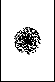
\includegraphics{assets/quasistatic/insets/inset_blob.pdf}};
					\end{axis}
				\end{tikzpicture}
				\caption[Quasi-static lesion density characterization]{Characterization of lesion density for a group of numerous smaller \SI{2}{\mm} diameter lesions comprising a large area with a diameter of \SI{2.5}{\cm} at a depth of \SI{10}{\cm} interrogated with a \SI{4}{\MHz} probing frequency and \SI{5}{\percent} applied strain. Detection sensitivity decreases with decreasing lesion density, as expected.}
				\label{fig:blob_density_characterization}
			\end{figure}

			The characterization plot in Fig. \ref{fig:blob_density_characterization} for small lesion density is less linear than other characterization plots, with lesion density having a significant effect on the detection sensitivity. Specifically, for low lesion densities, the detection sensitivity is much lower than for high lesion densities. However, this observation is warranted after examination of the elastogram produced from these results, given in Fig. \ref{fig:blob_elastogram}, which shows how the small lesions are not individually detected but rather the entire region is detected as one large lesion. Since the average stiffness ratio over this region is lesser than the stiffness ratio of individual lesions, it makes sense that the ``measured'' strain ratio will be less than expected.

			\begin{figure}[!htb]
				\centering
				\subfloat[]{
					\begin{tikzpicture}
						\begin{axis}[
							width=0.9\columnwidth,
							enlargelimits=false,
							unit vector ratio*=1 1 1,
							axis on top,
							xlabel={Lateral deviation, $x$ (\si{\cm})},
							ylabel={Depth, $d$ (\si{\cm})},
							y dir=reverse,
							draw=black, text=black, fill=black]
								\addplot graphics[xmin=-2,xmax=2,ymin=0,ymax=12.5]{assets/quasistatic/images/stiffnessMap_092_colour.png};
						\end{axis}
					\end{tikzpicture}
					\label{fig:blob_elastogram_a}
				}
				~
				\subfloat[]{
					\begin{tikzpicture}
						\begin{axis}[
							width=0.9\columnwidth,
							enlargelimits=false,
							unit vector ratio*=1 1 1,
							axis on top,
							xlabel={Lateral deviation, $x$ (\si{\cm})},
							ylabel={Depth, $d$ (\si{\cm})},
							y dir=reverse,
							colormap name={YlOrRd},
							colorbar,
							point meta min=0,
							point meta max=7,
							colorbar style={yticklabel={\pgfmathprintnumber{\tick}\,\si{\percent}}, at={(1.05,0)}, width=0.01\textwidth, ylabel={Compressive Strain}, anchor=south west,
							draw=black, text=black, fill=black},
							draw=black, text=black, fill=black]
								\addplot graphics[xmin=-2,xmax=2,ymin=0,ymax=12.5]{assets/quasistatic/elastograms/e092_colour.png};
						\end{axis}
					\end{tikzpicture}
					\label{fig:blob_elastogram_b}
				}
				\caption[Sample elastogram for a set of clustered lesions]{Stiffness map \protect\subref{fig:blob_elastogram_a} and corresponding elastogram \protect\subref{fig:blob_elastogram_b} for a group a small lesions with a density of 10 lesions per \SI{}{cm^2} grouped in a \SI{2.5}{\cm} diameter circle at a depth of \SI{10}{\cm} interrogated with a \SI{4}{\MHz} probing frequency and \SI{5}{\percent} applied strain. In \protect\subref{fig:blob_elastogram_a}, white regions are regular tissue while black regions are the small lesions. In the elastogram, individual lesions do not stand out, rather the entire region of lesions appears as one large region of unhealthy tissue.}
				\label{fig:blob_elastogram}
			\end{figure}

			\begin{figure}[!htb]
				\centering
				\begin{tikzpicture}
					\begin{axis}[
						scale only axis,
						height=3in,
						width=\textwidth-\widthof{100}-1in,
						xlabel={True Lesion Stiffness Ratio, $E_{true}$},
						ylabel={Measured Lesion Stiffness Ratio, $E_{meas}$},
						grid=major,
						legend entries={$r_{bl} = \SI{0.5}{\mm}$, $r_{bl} = \SI{1.0}{\mm}$, $r_{bl} = \SI{2.0}{\mm}$, $r_{bl} = \SI{2.5}{\mm}$},
						legend style={legend pos=north west,font=\small},
						clip=true,
						cycle list name=ColourPlotCycle,
						draw=black, text=black, fill=black]
							\addplot table {assets/quasistatic/data/blob_radius_05.dat};
							\addplot table {assets/quasistatic/data/blob_radius_10.dat};
							\addplot table {assets/quasistatic/data/blob_radius_15.dat};
							\node [anchor=south](c) at (axis cs:3.125,0.6) {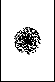
\includegraphics{assets/quasistatic/insets/inset_blob.pdf}};
					\end{axis}
				\end{tikzpicture}
				\caption[Quasi-static clustered lesion radius characterization]{Characterization of lesion radius for a group of numerous smaller lesions with a density of 30 lesions per \SI{}{cm^2} comprising a large area with a diameter of \SI{2.5}{\cm} at a depth of \SI{10}{\cm} interrogated with a \SI{4}{\MHz} probing frequency and \SI{5}{\percent} applied strain. Detection sensitivity decreases with decreasing individual lesion size, as expected.}
				\label{fig:blob_radius_characterization}
			\end{figure}

			Similar to the results shown in Fig. \ref{fig:blob_density_characterization}, changing the size of the individual small lesions does have an effect on the measured strain. In this case, when individual lesions are small, the total area occupied by lesions is lesser which results in a lesser average tissue stiffness over the grouped lesion region.

			Note that although the elastography algorithm was able to detect the larger lesion-filled regions in these simulations, it was completely unable to discern the individual lesions comprising those regions. This is not surprising due to both the generated strain fields in the healthy tissue throughout the larger lesion area as well as the results presented in Fig. \ref{fig:size_characterization} showing poor detection sensitivity for lesions with diameters $\leq \SI{1}{\cm}$ while the individual lesions in this simulation had diameters of the scale of \SI{0.5}{\mm} -- \SI{1.5}{\mm}.

			Finally, in order to place these results within the context of a likely real scenario in humans, a more complicated model utilizing an MRI-acquired lesion and slides from the Visible Human Project \cite{visiblehuman} was developed. Specifically, lesion geometry was taken from a real deep tissue injury in a pig model imaged using $\mathrm{T}_2^*$-weighted MRI. The human geometry was taken from a transverse plane slice aross the left ischial tuberosity such that the lesion was placed immediately superficial to the boney promience. For this model, the overall lesion width and lesion depth were examined with results shown in Figs. \ref{fig:human_size_characterization} and \ref{fig:human_depth_characterization} respectively.

			\begin{figure}[!htb]
				\centering
				\begin{tikzpicture}
					\begin{axis}[
						scale only axis,
						height=3in,
						width=\textwidth-\widthof{100}-1in,
						xlabel={True Lesion Stiffness Ratio, $E_{true}$},
						ylabel={Measured Lesion Stiffness Ratio, $E_{meas}$},
						grid=major,
						legend entries={$\diameter S = \SI{0.5}{\cm}$, $\diameter S = \SI{1.0}{\cm}$, $\diameter S = \SI{2.0}{\cm}$, $\diameter S = \SI{2.5}{\cm}$},
						legend style={legend pos=north west,font=\small},
						clip=true,
						cycle list name=ColourPlotCycle,
						draw=black, text=black, fill=black]
							\addplot table {assets/quasistatic/data/human_size_05.dat};
							\addplot table {assets/quasistatic/data/human_size_10.dat};
							\addplot table {assets/quasistatic/data/human_size_20.dat};
							\addplot table {assets/quasistatic/data/human_size_25.dat};
							\node [anchor=south](c) at (axis cs:3.2,0.7) {
\includegraphics[width=0.072\columnwidth]{assets/quasistatic/insets/human.png}};
							\node [anchor=south](rect) at (axis cs:3.2,0.72) [draw,minimum width=0.072\columnwidth,minimum height=0.18\columnwidth]{};
					\end{axis}
				\end{tikzpicture}
				\caption[Quasi-static Visible Human model lesion width characterization]{Characterization of lesion width in a Visible Human-MRI model for lesions at a depth of \SI{7.25}{\cm} interrogated with a \SI{4}{\MHz} probing frequency with \SI{5}{\percent} applied strain. Small lesions (with a width $\leq \SI{1.0}{\cm}$) are severely misrepresented and portray general over-estimation of lesion stiffness larger lesions.}
				\label{fig:human_size_characterization}
			\end{figure}

			In Fig. \ref{fig:human_size_characterization}, it is clear to see than small lesions (with a diameter $\leq \SI{1.0}{\cm}$) are almost impossible to adequately detect (although larger lesions will be adequately detectable). It is hypothesized that this phenomenon is due to the excessive strain apparent above the boney prominence that is seen in the resultant elastogram given in Fig. \ref{fig:human_elastogram} such that the lesion is ``washed out'' by the strain field developed by the relatively stiff bone nearby.

			\begin{figure}[!htb]
				\centering
				\begin{tikzpicture}
					\begin{axis}[
						width=\columnwidth,
						enlargelimits=false,
						unit vector ratio*=1 1 1,
						axis on top,
						xlabel={Lateral deviation, $x$ (\si{\cm})},
						ylabel={Depth, $d$ (\si{\cm})},
						y dir=reverse,
						colormap name={YlOrRd},
						colorbar,
						point meta min=0,
						point meta max=7,
						colorbar style={yticklabel={\pgfmathprintnumber{\tick}\,\si{\percent}}, at={(1.05,0)}, width=0.01\textwidth, ylabel={Compressive Strain}, anchor=south west,
						draw=black, text=black, fill=black},
						draw=black, text=black, fill=black]
							\addplot graphics[xmin=-2,xmax=2,ymin=0,ymax=10]{assets/quasistatic/elastograms/e117_colour.png};
					\end{axis}
				\end{tikzpicture}
				\caption[Sample elastogram of a Visible Human model lesion]{Elastogram for a \SI{0.5}{\cm} wide lesion embedded in the Visible Human-MRI model domain at a depth of \SI{7.25}{\cm} interrogated at \SI{4}{\MHz} with an applied strain of \SI{2.5}{\percent}. The lesion is not visible in the resultant elastogram.}
				\label{fig:human_elastogram}
			\end{figure}

			\begin{figure}[!htb]
				\centering
				\begin{tikzpicture}
					\begin{axis}[
						scale only axis,
						height=3in,
						width=\textwidth-\widthof{100}-1in,
						xlabel={True Lesion Stiffness Ratio, $E_{true}$},
						ylabel={Measured Lesion Stiffness Ratio, $E_{meas}$},
						grid=major,
						legend entries={$d = \SI{6.25}{\cm}$, $d = \SI{6.75}{\cm}$, $d = \SI{7.25}{\cm}$},
						legend style={legend pos=north west,font=\small},
						clip=true,
						cycle list name=ColourPlotCycle,
						draw=black, text=black, fill=black]
							\addplot table {assets/quasistatic/data/human_bottom_sep_625.dat};
							\addplot table {assets/quasistatic/data/human_bottom_sep_675.dat};
							\addplot table {assets/quasistatic/data/human_bottom_sep_725.dat};
							\node [anchor=south](c) at (axis cs:3.2,0.62) {
\includegraphics[width=0.072\columnwidth]{assets/quasistatic/insets/human.png}};
							\node [anchor=south](rect) at (axis cs:3.2,0.64) [draw,minimum width=0.072\columnwidth,minimum height=0.18\columnwidth]{};
					\end{axis}
				\end{tikzpicture}
				\caption[Quasi-static characterization of lesion depth in a Visible Human model]{Characterization of lesion depth in a Visible Human-MRI model for lesions with a width of \SI{2.5}{\cm} interrogated with a \SI{4}{\MHz} probing frequency and \SI{5}{\percent} applied strain. Deeper lesions (closer to the bony promience) are have slightly over-estimated lesion stiffness ratios as opposed to more superficial lesions while detection sensitivity is not affected by lesion depth.}
				\label{fig:human_depth_characterization}
			\end{figure}

			In Fig. \ref{fig:human_depth_characterization}, there is little to no dependence of the detection sensitivity on the lesion depth in the Visible Human-MRI model with all depth curves displaying the same profile. However, deeper lesions (lesions closer to the bony prominence) have stiffnesses that are over-estimated with respect to their superficial counterparts. This is hypothesized to be due to the increased strain field present in all of the soft tissue located immediately superior to the bony prominence, but should not pose a serious problem for imaging lesions of this nature.

		\subsection{Physical Phantom Validation}
			In order to ensure that the models presented here represented physical realities, a small subset of the cases studied were modelled in a physical phantom, specifically for three lesions with stiffness ratios of 0.56, 1.80, and 3.20 with a diameter of \SI{2.0}{\cm} and at a depth of \SI{3.5}{\cm}, interrogated at \SI{8}{\MHz} with approximately \SI{5}{\percent} applied strain. The results of this study are summarized in Fig. \ref{fig:phantom_validation}.

			\begin{figure}[!htb]
				\centering
				\begin{tikzpicture}
					\begin{axis}[
						scale only axis,
						height=3in,
						width=\textwidth-\widthof{100}-1in,
						xlabel={Simulated Measured Strain Ratio, $E_{sim,measured}$},
						ylabel style={align=center},
						ylabel={Experimental Measured \\ Stiffness Ratio, $E_{exp,measured}$},
						legend entries={Results, Ideal},
						legend style={legend pos=south east,font=\small},grid=major,clip=true,cycle list name=ColourPlotCycle,
						xmin=0.5, xmax=2.5,
						ymin=0.5, ymax=2.5,
						draw=black, text=black, fill=black]
							\addplot table {assets/quasistatic/data/validation.dat};
							\addplot[mark=none,dashed,ultra thick] table {assets/quasistatic/data/ideal_1_1.dat};
							\node [anchor=north west](c) at (axis cs:0.55,2.45) {
\includegraphics{assets/quasistatic/insets/inset_single.pdf}};
					\end{axis}
				\end{tikzpicture}
				\caption[Experimental validation of quasi-static model results]{Relation between simulated measured strain ratios and experimental measured strain ratios for a lesion at a depth of \SI{3.5}{\cm} and diameter of \SI{2.0}{\cm} showing general agreement between simulated and experimental cases. Idealization errors are the most likely the cause of the differences seen between simulated and experimental cases.}
				\label{fig:phantom_validation}
			\end{figure}

			As can be seen in Fig. \ref{fig:phantom_validation}, a relatively simple (although inexact) relationship between simulated and experimental measured strain ratios exists. It must be noted that the finite-element simulations of b-mode image formation and tissue deformation presented here are idealizations of reality and idealization errors such as the ultrasound pulse profile and plane-strain assumption no doubt contributed to the difference seen in Fig. \ref{fig:phantom_validation}.

			It must be noted that in order to acquire quasi-static elastography results in the physical phantom, the ultrasound transducer was required to be manually manipulated to cause indentation in the phantom, as the technique would most likely be performed in a clinical setting. This was found to be problematic as the ultrasound transducer was difficult to maintain perfectly perpendicular and in-plane during the compression (largely due to the necessity of using coupling ultrasonic gel). This difficulty suggests that acoustic radiation force impulse (ARFI) elastography would be a more appropriate method to acquire DTI elastograms. ARFI elastography works on the same principles as quasi-static elastography with the exception that tissue deformation is caused by localized large-amplitude acoustic waves generated by the transducer such that human factors play a far less substantial role in image acquisition.

	\section{Conclusion}
		This work represents a numerical characterization of the use of quasi-static ultrasound elastography for the early detection of deep tissue injuries (DTI). There is a real clinical need for an objective tool that is capable of detecting the formation and progression of DTI in human subjects as these wounds are generally not visible from the surface of the skin until they have broken through and already caused substantial damage.

		Through the numerical characterization, quasi-static ultrasound elastography was found to be an effective tool for detecting and monitoring DTI in theoretical simulations. Overall, detection sensitivity was less than expected. Small lesions (with diameters $\leq \SI{1.0}{\cm}$) were more difficult to differentiate due to the low lesion detection sensitivity. While lesion depth, altitude above the underlying bone, and probing frequency did not have significant effect on the lesion detection sensitivity, it was found that applying high levels of compressive strain (\SI{10}{\percent}) introduced severe error for both very soft and very stiff lesions, thus it is recommended that diagnosticians only apply moderate ($\leq \SI{5}{\percent}$) compressive strain when interrogating potential lesions. Larger strains may alternately be induced by slowly palpating the tissue with very minor strains frame-by-frame and cumulating the displacement fields across these smaller palpations. Care must be used when palpating the tissue, lest ``vigorous'' palpations cause harm to the already sensitive injury. In the more complicated model of co-located lesions, while the separation distance between adjacent lesions did not affect the detection sensitivity, the placing of adjacent lesions generated ``phantom'' lesion regions with altered strain that may appear to be diseased tissue when they are in fact healthy. In a model lesion with gradual blurred boundaries, the effect of blur radius only affected the detection sensitivity and ability to differentiate soft lesions. Specifically, soft lesions with large blur radii became nearly impossible to differentiate as these lesions all showed a measured lesion stiffness ratio of approximately 1 which would show up as regular, healthy tissue. In the case of numerous clustered small lesions, both decreased lesion density and decreased individual lesion size caused a decrease in lesion detection sensitivity, likely due to the averaging effect of healthy tissue and diseased tissue in near proximity. Finally, in the Visible Human-MRI acquired lesion model, lesions with widths $\leq \SI{1.0}{\cm}$ are nearly impossible to differentiate as they are hidden by the strain field generated by the bony prominence. Lesion depth did not have an effect on the detection sensitivity, though deeper lesions (lesions which were closer to the bony prominence) had overestimated stiffnesses with respect to their more superficial counterparts.

		Although the studies presented here resulted in less-than-ideal detection sensitivities, the technique was still able to pick out lesions from the surrounding soft (and hard) tissue. Work done by Solis et al. \cite{solis13} has shown that untreated DTI are multiple centimeters in size, while work done by Gefen et al. \cite{gefen05} has shown that deep tissue injuries exhibit 1.8-fold to 3.3-fold mechanical stiffening. The work presented here has shown that quasi-static ultrasound elastography is adequate at detecting deep tissue injury lesions in these ranges of parameters and will thus be adequate to detect and monitor progress DTI. However, without further real-world experimentation on the exact nature of newly-forming DTI, the detection sensitivity required to detect newly-forming DTI is indeterminate.

		A subset of the results found through simulation were compared with similar experiments done using a tissue mimicking phantom model. The experimental results using the phantom model generally agreed with those found from simulation cases. It was also noted that the manual skin indentation technique involved with quasi-static ultrasound elastography proved to be difficult to produce reliable images. This difficulty suggests that an alternate method of performing ultrasound elastography may be preferable to quasi-static ultrasound elastography with manual indentation. Acoustic radiation force impulse (ARFI) elastography may be a more appropriate method to acquire DTI elastograms as although ARFI elastography works on the same principles as quasi-static elastography, the difference lays in the fact that tissue deformation is caused by localized large-amplitude acoustic waves generated by the transducer. This means that human factors play a far less substantial role in image acquisition and would likely improve repeatability and inter-operator reliability. Nevertheless, the work done here to characterize the use of quasi-static ultrasound elastography is an important step along the path of generating a useful clinical tool for detecting formative and monitoring progressive deep tissue injuries.

\comment{
	\cleardoublepage

	\phantomsection

	\addcontentsline{toc}{section}{References}
	\bibcomplete{references}
	\printbibliography[heading=subbibliography]
}
\chapter{Numerical Characterization of Acoustic Radiation Force Impulse Imaging}
	\label{chap:arfi}
	\section{Introduction}
		Acoustic radiation force impulse imaging presents a chief benefit over quasi-static ultrasound elastography in that since the external deformation force is applied by the transducer itself rather than through manual indentation of the transducer by the diagnostician, the inter-operator reliability may be greatly increased. The net effect of this is an expected decrease in the required amount of training of diagnosticians as well as an expected increase in the sensitivity and specificity of early deep tissue injury detection.

	\section{Method}
	\label{sec:arfi_methods}
		In order to numerically characterize acoustic radiation force impulse imaging for the early detection of deep tissue injuries, a combinatory model of acoustic radiation force simulations and time-domain finite-element models of tissue deformation were used. Acoustic radiation force distributions were calculated using a k-space pseudospectral model of ultrasonic acoustics which simulated the acoustic intensities and subsequent radiation force developed by an ultrasonic transducer applying deep body loads to soft tissue. These forces were then combined with a temporal finite-element model of tissue deformation to model the response of the tissue to the body force impulses generated by the transducer. The use of these models allowed extensive simulation and parameter sensitivity analysis in order to numerically characterize the use of 

		\subsection{K-Space Pseudospectral Model of Acoustic Fields}
		\label{subsec:kspace_model}
			In order to simulate the body loads generated within deep tissue by a continuous ultrasound beam, a k-space pseudospectral model of acoustic field intensities was generated. The body load fields that were generated as a result of this model were fed into a temporal soft tissue deformation model to investigate the dynamic response of tissue to ARFI loads.

			The governing equations used for the k-space pseudospectral model were the set of coupled first-order partial differential equations \ref{equ:arfi_gov_p1} -- \ref{equ:arfi_gov_p3}. These equations are the first-order equivalents of the wave equation given in equation \ref{equ:wave_equation} taking into account acoustic absorption, tissue heterogeneities, and acoustic wave non-linearities \cite{treeby12}. Equations \ref{equ:arfi_gov_p1}, \ref{equ:arfi_gov_p2}, and \ref{equ:arfi_gov_p3} represent the momentum conservation, mass conservation, and pressure-density relation terms respectively.

			\begin{subequations}
				\label{equ:arfi_gov}
				\begin{align}
					\frac{\partial \vec{u}}{\partial t} &= - \frac{1}{\rho_0} \nabla p \label{equ:arfi_gov_p1} \\
					\frac{\partial p}{\partial t} &= -\left(2 \rho + \rho_0\right)\nabla \cdot \vec{u} - \vec{u} \cdot \nabla \rho_0 \label{equ:arfi_gov_p2} \\
					p &= c_0^2 \left(\rho + \vec{d} \cdot \nabla \rho_0 + \frac{B}{2A} \frac{\rho^2}{\rho_0} - \mathbf{L}\rho \right) \label{equ:arfi_gov_p3}
				\end{align}
			\end{subequations}

			\note[KH]{Talk about all the parameters in these equations}

			\begin{equation}
				\label{equ:wave_equation}
				\nabla^2 p - \frac{1}{c_0^2}\frac{\partial^2 p}{\partial t^2} = 0
			\end{equation}

			The $\mathbf{L}$ operator used in equation \ref{equ:arfi_gov_p3} accounts for acoustic absorption and dispersion which follows a frequency power law and is defined as per equations \ref{equ:Lop1} -- \ref{equ:Lop3}.

			\begin{subequations}
				\begin{align}
					\mathbf{L} &= \tau \frac{\partial}{\partial t}\left(-\nabla^2\right)^{\frac{y}{2} - 1} + \eta \left(-\nabla^2\right)^{\frac{y+1}{2} - 1} \label{equ:Lop1} \\
					\tau &= -2\alpha_0 c_0^{y-1} \label{equ:Lop2} \\
					\eta &= 2\alpha_0c_0^y\tan\left(\frac{\pi y}{2}\right)  \label{equ:Lop3}
				\end{align}
			\end{subequations}

			In order to integrate pressure sources in equations \ref{equ:arfi_gov_p1} -- \ref{equ:arfi_gov_p3}, equation \ref{equ:arfi_gov_p2} is modified to include a mass source term, $S_M$ which counts as a pressure source term through changing density to form equation \ref{equ:arfi_gov_p2_source}.

			\begin{equation}
				\label{equ:arfi_gov_p2_source}
				\frac{\partial p}{\partial t} = -\left(2 \rho + \rho_0\right)\nabla \cdot \vec{u} - \vec{u} \cdot \nabla \rho_0 + S_M
			\end{equation}

			The k-Wave MATLAB\textsuperscript{\textregistered} toolbox version 1.0 was used to solve for the time-variant intensities resulting from simulated acoustic radiation force impulses applied to heterogeneous soft tissue using equations \ref{equ:arfi_gov_p1}, \ref{equ:arfi_gov_p2_source}, and \ref{equ:arfi_gov_p3}. Sample source code for performing these simulations using the k-Wave toolbox is given in listing \ref{lst:intensity} in Appendix \ref{app:source_code}.

		\subsection{Derivation of Acoustic Radiation Force}
		\label{subsec:body_load_derivation}
			Acoustic radiation force arises as the result of absorption of linear momentum within tissue as acoustic waves travel though it with the requirement that the tissue is a viscoelastic medium---no energy would be absorbed in a purely linear elastic model. Further, at the super-\si{\MHz} frequencies involved in ultrasound interrogation, tissue may be considered a viscous fluid \note[KH]{Add citation!}.

			\comment{For a linearly viscous fluid, the constitutive relationship is given in equation \ref{equ:constitutive_linear_viscous} where $D_{ij}$ is defined as per equation \ref{equ:rate_deformation_linear_viscous} and represents the rate of deformation.

			\begin{equation}
				\label{equ:constitutive_linear_viscous}
				\sigma_{ij} = -p \delta_{ij} + \lambda_f D_{ii} \delta_{ij} + 2 \mu_f D_{ij}
			\end{equation}

			\begin{equation}
				\label{equ:rate_deformation_linear_viscous}
				D_{ij} = \frac{1}{2}\left(v_{i,j} + v_{j,i}\right)
			\end{equation}

			\note[KH]{Describe symbols!}

			Beginning with the Navier-Stokes equation for an incompressible Newtonian fluid given in equation \ref{equ:navier_stokes}, the acoustic radiation force may be derived given that $\mu_f$ in equation \ref{equ:navier_stokes} represents an energy loss related the an attenuation coefficient, $\alpha$ \cite{kino87}.

			\begin{equation}
				\label{equ:navier_stokes}
				-p_{,i} + \mu_f v_{i,jj} + \rho b_i = \rho\left(\dot{v_i} + v_j v_{i,j}\right)
			\end{equation}}

			Using a perturbative expansion of equation \ref{equ:arfi_linear_momentum}, acoustic radiation force can be expressed as per equations \ref{equ:radiation_force_1} \cite{nyborg65}. In equations \ref{equ:radiation_force_1}, $\langle\rangle$ represents the time-average operator, $\vec{v_1}$ and $\vec{v_2}$ are the first and second order terms in the perturbative expansion of particle velocity, and $p_2$ is the second order pressure term in the perturbative expansion, while $\vec{F}$ represents the acoustic radiation force developed in the tissue.

			\begin{equation}
				\label{equ:arfi_linear_momentum}
				\sigma_{ij,j} + \rho b_i = \rho f_i
			\end{equation}

			\begin{subequations}
				\label{equ:radiation_force_1}
				\begin{align}
					\vec{F} &= \nabla p_2 - \mu_f \nabla^2 \vec{v_2} \label{equ:radiation_force_1a} \\
					\vec{F} &= \rho \langle\vec{v_1}\nabla\cdot\vec{v_1} + \vec{v_1}\nabla\vec{v_1}\rangle \label{equ:radiation_force_1b}
				\end{align}
			\end{subequations}

			For a plane wave, equation \ref{equ:radiation_force_1b} can be reduced to equation \ref{equ:radiation_force_2}. Further, substituting the generalized wave particle velocity solution given in equation \ref{equ:particle_velocity} in equation \ref{equ:radiation_force_2}, the magnitude of acoustic radiation force may be calculated as per equation \ref{equ:radiation_force_3}.

			\begin{equation}
				\label{equ:radiation_force_2}
				\vec{F} = 2\rho\langle \vec{v} \vec{v}_{,x} \rangle
			\end{equation}

			\begin{equation}
				\label{equ:particle_velocity}
				\vec{v} = i\omega A e^{-\alpha x + i\left(\omega t - k x\right)}\hat{x}
			\end{equation}

			\begin{equation}
				\label{equ:radiation_force_3}
				\left|\vec{F}\right| = A^2 e^{-2\alpha x}\rho\alpha
			\end{equation}

			Further using the acoustic field intensity, the acoustic radiation force may be calculated as per equation \ref{equ:radiation_force} where $\alpha$ is the absorption coefficient of the tissue in \si{\neper\per\m}, $I$ is the temporal average acoustic intensity in \si{\W\per\m\squared}, and $c$ is the longitudinal speed of sound in the tissue in \si{\m\per\s} \cite{palmeri05}.

			\begin{equation}
				\label{equ:radiation_force}
				\left|\vec{F}\right| = \frac{2\alpha I}{c}
			\end{equation}

			Once acoustic radiation force body loads were calculated as per equation \ref{equ:radiation_force}, they were used as initial conditions to the temporal finite-element model of soft tissue deformation described in Section \ref{subsec:temporal_fea_arfi}.

		\subsection{Temporal Finite-Element Model of Soft Tissue Deformation}
			\label{subsec:temporal_fea_arfi}
			In response to the relatively short duration (``impulse'') acoustic radiation force body load applied to tissue in ARFI imaging, the interrogated tissue will exhibit a dynamic response---namely that tissue deformation will propagate outwards as the absorbed acoustic energy diffuses through the soft tissue.

			In order to simulate the dynamic tissue deformation generated by the acoustic impulse force, a generalized Maxwell viscoelastic model of tissue deformation was used \cite{then12}. The simulated tissue properties are summarized in Tables \ref{tab:arfi_properties} and \ref{tab:arfi_maxwell_properties}.

			\begin{table}[!htb]
				\centering
				\caption{ARFI Model Viscoelastic Tissue Properties}
				\label{tab:arfi_properties}
				\begin{tabular}{lrs[table-unit-alignment = left]}
					\toprule
					Property & Value & Units \\
					\midrule
					Bulk Modulus & 515.7 & \si{\kPa} \\
					Shear Modulus & 1.0 & \si{\kPa} \\
					Density & 1060 & \si{\kg\per\m\cubed} \\
					\bottomrule
				\end{tabular}
			\end{table}

			\begin{table}[!htb]
				\centering
				\caption{ARFI Maxwell Model Tissue Properties}
				\label{tab:arfi_maxwell_properties}
				\begin{tabular}{lrr}
					\toprule
					Branch & Shear Modulus & Relaxation Time \\
					& (\si{\Pa}) & (\si{\s}) \\
					\midrule
					1 & 791.0 & 2 \\
					2 & 66.5 & 40 \\
					3 & 0.6 & 80 \\
					\bottomrule
				\end{tabular}
			\end{table}

			% 1 791 2
			% 2 66.5 40
			% 3 0.628 80

			%the time-dependent displacement field was calculated according to equation \ref{fea:time_deformation} where \note[KH]{Don't leave us hanging!}.
			\comment{The time-dependent displacement fields were calculated according to equations \ref{fea:time_deformation} where $\sigma$ is the Cauchy stress tensor, $\vec{F}$ are the applied body forces, $\vec{u}$ is the particle displacement, $S_0$ is the initial stress distribution, $p_w$ is ?, $\vec{I}$ is the identity matrix, $G$ the shear modulus, $q_m$ is an auxiliary strain variable used to represent the extension of the $m$-th abstract string, $varepsilon$ is strain, and $t$ is time. Lesions were modeled identically to the rest of the soft tissue with the exception of the bulk and shear moduli being some fraction or multiple of the ``healthy'' moduli.

			\begin{subequations}
				\label{fea:time_deformation}
				\begin{align}
					\vec{F} &= \rho \ddot{\vec{u}} - \nabla \cdot \sigma \\
					\sigma - S_0 &= - p_w \vec{I} + 2 G\left(\varepsilon - \varepsilon_0 - \frac{1}{3} tr(\varepsilon - \varepsilon_0)\vec{I}\right) + \sum_{m=1}^N 2G_m q_m \\
					\dot{q}_m + \frac{1}{\tau_m} q_m &= \frac{\partial}{\partial t}\left(\varepsilon - \varepsilon_0 - \frac{1}{3} tr(\varepsilon - \varepsilon_0)\vec{I}\right)
				\end{align}
			\end{subequations}}

			The time-dependent displacement fields were calculated according to equation \ref{fea:time_deformation} where $\sigma$ is the Cauchy stress tensor, $\vec{F}$ are the applied body forces, and $\vec{u}$ is the particle displacement, and $\rho$ is the density.

			\begin{equation}
				\label{fea:time_deformation}
				%\vec{F} = \rho \ddot{\vec{u}} - \nabla \cdot \sigma
				\rho \frac{\partial^2 \vec{u}}{\partial t^2} - \nabla \cdot \sigma = \vec{F}
			\end{equation}

			In order to include viscoelastic effects through a generalized Maxwell model of soft tissue, equation \ref{fea:time_deformation_visco} was used where $\sigma_0$ is the initial stress distribution in the tissue, $C$ is the $4^{\text{\tiny th}}$ order elasticity tensor, $\varepsilon$ is the strain, $G_m$ and $\tau_m$ are the shear modulus and relaxation time of the $m^{\text{\tiny th}}$ branch of the Maxwell model respectively, and $\gamma_m$ is an additional auxillary degree of freedom used to represent the extension of the abstract springs in the Maxwell model.

			\begin{equation}
				\label{fea:time_deformation_visco}
				\sigma - \sigma_0 = C : \varepsilon + \sum_m 2 G_m \tau_m \dot{\gamma}_m 
			\end{equation}

			In the simulations, the boundary equations \ref{equ:arfi_fea_fixed_bc} were used to apply a fixed boundary condition to the both the bottom (deep) and top (superficial) boundaries of the model in the axial direction at both boundaries and in the lateral direction at the deep boundary. All other boundaries of the model were free to translate in all dimensions. The acoustic radiation force was applied as a body load to the tissue in the model with the distribution calculated by the k-space pseudospectral model and resultant body forces described in Sections \ref{subsec:kspace_model} and \ref{subsec:body_load_derivation}. In order to prevent reflections from the model boundaries that might affect the simulation results, the model geometry extended laterally by \SI{5}{\cm} in either direction from the centerline. Simulations were run until the axial displacement at the focal point returned to \SI{1}{\percent} of it's maximal value during the entire simulation---at this point, the tissue was considered to be ``relaxed'' after being disturbed by the acoustic radiation force.

			\begin{subequations}
				\label{equ:arfi_fea_fixed_bc}
				\begin{align}
					\vec{u} &= 0, \qquad \Gamma = \Gamma_{bottom} \\
					u_y &= 0, \qquad \Gamma = \Gamma_{top}
				\end{align}
			\end{subequations}

		\subsection{Characterizing Acoustic Radiation Force Impulse Imaging}
			%In order to fully understand the suitability of using ARFI imaging to detect and monitor deep tissue injuries, 5 general models of deep tissue injury lesions were modeled. Each general model was also investigated over a range of parameters in order to determine the relationship between the detection sensitivity and the various parameters that were studied. The investigated models included a model with hard boundaries

			\begin{figure*}[!htb]
				\centering
				\subfloat[]{
					\begin{tikzpicture}[x=0.045\textwidth, y=0.045\textwidth, draw=black, text=black, fill=black]
						% the main domain area
						\draw[fill=tissueColour] (0, 0) rectangle(10, 10);

						% the lesion
						\draw[fill=lesionColour] (5, 6) circle(0.5);

						% the lesion center marks
						\draw (4.4, 6) -- (4.9, 6);
						\draw (5.1, 6) -- (5.6, 6);
						\draw (4.95, 6) -- (5.05, 6);
						\draw (5, 5.4) -- (5, 5.9);
						\draw (5, 6.1) -- (5, 6.6);
						\draw (5, 5.95) -- (5, 6.05);

						% the lesion radius
						\draw[<-] (5.3536, 5.6464) -- (6, 5);
						\draw (5.85, 5) node[right]{\scriptsize $\diameter S$};

						% the lesion depth
						\draw (4, 6) -- (4.5, 6);
						\draw[<-] (4.25, 10) -- (4.25, 8.25);
						\draw (4.25, 8) node{\scriptsize $d$};
						\draw[->] (4.25, 7.75) -- (4.25, 6);

						% the domain width
						\draw (0, 10.1) -- (0, 10.5);
						\draw[<-] (0, 10.25) -- (4.25, 10.25);
						\draw (5, 10.25) node{\scriptsize \SI{10}{\cm}};
						\draw[->] (5.75, 10.25) -- (10, 10.25);
						\draw (10, 10.1) -- (10, 10.5);

						% the domain depth
						\draw (10.1, 0) -- (11, 0);
						\draw[<-] (10.75, 0) -- (10.75, 4.75);
						\draw (10.75, 5) node{\scriptsize \SI{10}{\cm}};
						\draw[->] (10.75, 5.25) -- (10.75, 10);
						\draw (10.1, 10) -- (11, 10);

					\end{tikzpicture}
					\label{fig:arfi_schematic_single}
				}
				~
				\subfloat[]{
					\begin{tikzpicture}[x=0.045\textwidth, y=0.045\textwidth, draw=black, text=black, fill=black]
						% the main domain area
						\draw[fill=tissueColour] (0, 0) rectangle(10, 10);

						% the lesion
						\draw (5, 6) node{
\includegraphics[width=0.045\textwidth]{assets/arfi/images/blurredLesion.png}};
						\draw (5, 6) circle(0.5);

						% the lesion radius
						\draw[<-] (5.3536, 5.6464) -- (6, 5);
						\draw (5.85, 5) node[right]{\scriptsize $\diameter S$};

					\end{tikzpicture}
					\label{fig:arfi_schematic_blur}
				}
				
				\subfloat[]{
					\begin{tikzpicture}[x=0.045\textwidth, y=0.045\textwidth, draw=black, text=black, fill=black]
						% the main domain area
						\draw[fill=tissueColour] (0, 0) rectangle(10, 10);

						% the lesion
						\draw (5, 6) node{\includegraphics[width=0.045\textwidth]{assets/arfi/images/clusteredLesion.png}};
						\draw (5, 6) circle(0.5);

						% the lesion radius
						\draw[<-] (5.3536, 5.6464) -- (6, 5);
						\draw (5.85, 5) node[right]{\scriptsize $\diameter S$};

						% blob size
						\draw[<-] (4.9, 5.9) -- (4, 5) node[left]{\scriptsize $r_{bl}$};

					\end{tikzpicture}
					\label{fig:arfi_schematic_clustered}
				}
				~
				\subfloat[]{
					\begin{tikzpicture}[x=0.045\textwidth, y=0.045\textwidth, draw=black, text=black, fill=black]
						% the human stuffz
						\draw (5, 5) node{
\includegraphics[width=0.45\textwidth]{assets/arfi/images/humanSchematic.png}};

						% the main domain area
						\draw (0, 0) rectangle(10, 10);

						% the depth
						\draw (6, 4) -- (6.75, 4);
						\draw (6.5, 7) node{\scriptsize $d$};
						\draw[<-] (6.5, 10) -- (6.5, 7.25);
						\draw[->] (6.5, 6.75) -- (6.5, 4);

						% the size
						\draw (3.75, 4.7) -- (3.75, 5.5);
						\draw (6.25, 4.7) -- (6.25, 5.5);
						\draw (4.875, 5.25) node{\scriptsize $\diameter S$};
						\draw[<-] (3.75, 5.25) -- (4.5, 5.25);
						\draw[->] (5.25, 5.25) -- (6.25, 5.25);

					\end{tikzpicture}
					\label{fig:arfi_schematic_human}
				}
				\caption[]{Schematics of the lesion models that were investigated using acoustic radiation force impulse imaging showing \protect\subref{fig:arfi_schematic_single} a spherical hard-boundaried lesion, \protect\subref{fig:arfi_schematic_blur} a spherical blurred-boundary lesion, \protect\subref{fig:arfi_schematic_clustered} a cluster of numerous small lesions composing a larger lesionous region, and \protect\subref{fig:arfi_schematic_human} the geometry from an MRI-acquired deep tissue injury overlaid on a slice from the Visible Human Project such that the injury lesion was located immediately superior to an ischial tuberosity.}	
				\label{fig:arfi_schematics}
			\end{figure*}

			\begin{table}[!htb]
				\centering
				\caption[ARFI model investigated parameters]{Range of values of investigated parameters}
				\label{tab:arfi-parametervalues}
				\begin{tabular}{lcc}
					\toprule
					Parameter & Symbol & Values \\
					\midrule
					ARFI probing frequency & $f$ & $[1, 2, 4, 6]$\,\si{\MHz} \\
					Transducer width & $w_{trans}$ & $[4, 8, 10]$\,\si{\cm} \\
					ARFI pulse cycles & $n_c$ & $[3, 100, 300, 500, 700]$ \\
					ARFI source pressure & $P_{source}$ & $[4, 5, 6, 7, 8]$\,\si{\MPa} \\
					Lesion depth & $d$ & $[1, 2, 3, 4, 5, 6, 7, 8, 9]$\,\si{\cm} \\
					Lesion diameter & $\diameter S$ & $[1.0, 2.0]$\,\si{\cm} \\
					Lesion stiffness ratio & $E_{rel}$ & $[0.32, 0.56, 1.80, 3.20]$ \\
					Blurred lesion blur radius & $b_r$ & $[1.0, 2.5, 5.0, 7.5]$\,\si{\mm} \\
					Clustered lesion density & $b_\rho$ & $[10, 20, 30, 40]$\,\si{\per\cm\squared} \\
					Clustered lesion radius & $r_{bl}$ & $[0.5, 1.0, 1.5]$\,\si{\mm} \\
					Visible human lesion width & $\diameter S$ & $[0.5, 1.0, 2.0, 2.5]$\,\si{\cm} \\
					Visible human lesion depth & $d$ & $[6.25, 6.75, 7.25]$\,\si{\cm} \\
					\bottomrule
				\end{tabular}
			\end{table}

		\FloatBarrier
		\subsection{Physical Phantom Validation}
			The same CIRS Elasticity QA Phantom model 049 that was used in the quasi-static studies described in Chapter \ref{chap:quasi-static} was used to experimentally validate a subset of the ARFI simulations described here. Using a Siemens ACUSON S2000 \note[KH]{Correct naming / registered marks / etc?} portable ultrasound machine with a Siemens 9L4 \note[KH]{Describe probe better} transducer, ARFI images were acquired of lesions within the phantom. \note[KH]{More?}

	\section{Results}
		Using the k-space pseudospectral model of ultrasound acoustics described in Section \ref{subsec:kspace_model}, acoustic radiation force distributions were acquired and analyzed for a range of input parameters. These force distributions were then fed into the time-domain finite-element model of soft tissue deformation described in Section \ref{subsec:temporal_fea_arfi} to examine the difference in relationships between the true and measured tissue stiffness ratios due to the various lesion and transducer parameters listed in Table \ref{tab:arfi-parametervalues}. The results obtained through this methodology were then compared to ARFI images taken with a commercial ultrasound machine. \note[KH]{This is terrible.}

		\subsection{K-Space Pseudospectral Models of Acoustic Radiation Force}
		\label{subsec:kspace_results}
			\begin{figure}[!htb]
				\centering
				\subfloat[]{
					\begin{tikzpicture}
						\begin{axis}[
							scale only axis,
							enlargelimits=false,
							unit vector ratio*=1 1 1,
							height=3in,
							y dir=reverse,
							xlabel={X-Coordinate, $x$ (\si{\cm})},
							ylabel={Depth, $d$ (\si{\cm})},
							axis on top,
							colormap name={RdBu},
							colorbar, point meta min=-175, point meta max=175, colorbar style={at={(1.05,0)}, anchor=south west, width=0.03\textwidth, ylabel={Acoustic Radiation Force, $F_{ARFI}$ (\si{\kN\per\metre\cubed})},
							draw=black, text=black, fill=black}]
								\addplot graphics[xmin=-2,xmax=2,ymin=0,ymax=10]{assets/shear/data/Fx158.png};
						\end{axis}
					\end{tikzpicture}
					\label{fig:arfi_forces_fx}
				}~
				\subfloat[]{
					\begin{tikzpicture}
						\begin{axis}[
							scale only axis,
							enlargelimits=false,
							unit vector ratio*=1 1 1,
							height=3in,
							y dir=reverse,
							xlabel={X-Coordinate, $x$ (\si{\cm})},
							axis on top,
							colormap name={RdBu},
							colorbar, point meta min=-175, point meta max=175, colorbar style={at={(1.05,0)}, anchor=south west, width=0.03\textwidth, ylabel={Acoustic Radiation Force, $F_{ARFI}$ (\si{\kN\per\metre\cubed})},
							draw=black, text=black, fill=black}]
								\addplot graphics[xmin=-2,xmax=2,ymin=0,ymax=10]{assets/shear/data/Fy158.png};
						\end{axis}
					\end{tikzpicture}
					\label{fig:arfi_forces_fy}
				}

				\subfloat[]{
					\begin{tikzpicture}
						\begin{axis}[
							scale only axis,
							enlargelimits=false,
							unit vector ratio*=1 1 1,
							height=3in,
							y dir=reverse,
							xlabel={X-Coordinate, $x$ (\si{\cm})},
							axis on top,
							colormap name={RdBu},
							colorbar, point meta min=-175, point meta max=175, colorbar style={at={(1.05,0)}, anchor=south west, width=0.03\textwidth, ylabel={Acoustic Radiation Force, $F_{ARFI}$ (\si{\kN\per\metre\cubed})},
							draw=black, text=black, fill=black}]
								\addplot graphics[xmin=-2,xmax=2,ymin=0,ymax=10]{assets/shear/data/F158.png};
						\end{axis}
					\end{tikzpicture}
					\label{fig:arfi_forces_fsum}
				}
				\caption[Sample acoustic radiation force distribution]{Sample acoustic radiation force distribution in the \protect\subref{fig:arfi_forces_fx} lateral and \protect\subref{fig:arfi_forces_fy} axial directions, and \protect\subref{fig:arfi_forces_fsum} the resultant $L^2$-norm generated by a \SI{2}{\MHz} transducer operating with an aperture of \SI{4}{cm} focusing an acoustic beam at a depth of \SI{4}{\cm} continuously for \SI{150}{\us} applying a pressure of \SI{3.35}{\MPa}.}
				\label{fig:arfi_forces}
			\end{figure}

			\begin{figure}[!htb]
				\centering
				\begin{tikzpicture}
					\begin{axis}[
						scale only axis,
						height=3in,
						width=\textwidth-\widthof{100}-1in,
						xlabel={Focal Depth, $d_{f}$ (\si{\cm})},
						ylabel={Body Force at Focal Point, $F_{b,f}$ (\si{\newton\per\metre\cubed})},
						grid=major,
						legend entries={$f = \SI{1}{\MHz}$, $f = \SI{2}{\MHz}$, $f = \SI{4}{\MHz}$, $f = \SI{6}{\MHz}$},
						legend style={legend pos=north east,font=\small},
						clip=true,
						cycle list name=ColourPlotCycle,
						draw=black, text=black, fill=black]
						\addplot table {assets/arfi/data/depth_force_freq1.dat};
						\addplot table {assets/arfi/data/depth_force_freq2.dat};
						\addplot table {assets/arfi/data/depth_force_freq4.dat};
						\addplot table {assets/arfi/data/depth_force_freq6.dat};
					\end{axis}
				\end{tikzpicture}
				\caption[Lessening of ARFI with increasing depth and probing frequency]{Lessening of ARFI with increasing depth and probing frequency}
				\label{fig:freq-depth-force}
			\end{figure}

			\begin{figure}[!htb]
				\centering
				\begin{tikzpicture}
					\begin{axis}[
						scale only axis,
						height=3in,
						width=\textwidth-\widthof{100}-1in,
						xlabel={Focal Depth, $d_{f}$ (\si{\cm})},
						ylabel={Spatial-Peak Pulse-Average Intensity, $I_{SPPA.3}$ (\si{\watt\per\cm\squared})},
						grid=major,
						legend entries={$f = \SI{1}{\MHz}$, $f = \SI{2}{\MHz}$, $f = \SI{4}{\MHz}$, $f = \SI{6}{\MHz}$},
						legend style={legend pos=north east,font=\small},
						clip=true,
						cycle list name=ColourPlotCycle,
						draw=black, text=black, fill=black]
						\addplot table {assets/arfi/data/depth_isppa_freq1.dat};
						\addplot table {assets/arfi/data/depth_isppa_freq2.dat};
						\addplot table {assets/arfi/data/depth_isppa_freq4.dat};
						\addplot table {assets/arfi/data/depth_isppa_freq6.dat};
						%\addplot[mark=none,dashed,ultra thick] plot coordinates {(1, 190) (9, 190)};
					\end{axis}
				\end{tikzpicture}
				\caption[$I_{SPPA.3}$ safety measures of ARFI pulses]{$I_{SPPA.3}$ safety measures of ARFI pulses}
				\label{fig:freq-depth-isppa}
			\end{figure}

			\begin{figure}[!htb]
				\centering
				\begin{tikzpicture}
					\begin{axis}[
						scale only axis,
						height=3in,
						width=\textwidth-\widthof{100}-1in,
						xlabel={ARFI Frequency, $f_{ARFI}$ (\si{\MHz})},
						ylabel={Body Force at Focal Point, $F_{b,f}$ (\si{\newton\per\metre\cubed})},
						grid=major,
						legend entries={$w_{trans} = \SI{4}{\cm}$, $w_{trans} = \SI{8}{\cm}$, $w_{trans} = \SI{10}{\cm}$},
						legend style={legend pos=north east,font=\small},
						clip=true,
						cycle list name=ColourPlotCycle,
						draw=black, text=black, fill=black]
						\addplot table {assets/arfi/data/freq_force_width4.dat};
						\addplot table {assets/arfi/data/freq_force_width8.dat};
						\addplot table {assets/arfi/data/freq_force_width10.dat};
					\end{axis}
				\end{tikzpicture}
				\caption[Lack of transducer width effect on focal force]{Lack of transducer width effect on focal force}
				\label{fig:trans-width-force}
			\end{figure}

			\begin{figure}[!htb]
				\centering
				\begin{tikzpicture}
					\begin{axis}[
						scale only axis,
						height=3in,
						width=\textwidth-\widthof{100}-1in,
						xlabel={Pulse Cycles, $n_c$},
						ylabel={Body Force at Focal Point, $F_{b,f}$ (\si{\newton\per\metre\cubed})},
						grid=major,
						clip=true,
						cycle list name=ColourPlotCycle,
						draw=black, text=black, fill=black]
						\addplot table {assets/arfi/data/pulse_cycles.dat};
					\end{axis}
				\end{tikzpicture}
				\caption[Lack of effect of pulse cycles on force at focal point]{Lack of effect of pulse cycles on force at focal point}
				\label{fig:pulse_cycles_force}
			\end{figure}

			\begin{figure}[!htb]
				\centering
				\begin{tikzpicture}
					\begin{axis}[
						scale only axis,
						height=3in,
						width=\textwidth-\widthof{100}-1in,
						xlabel={Focal Depth, $d_f$ (\si{\cm})},
						ylabel={Body Force at Focal Point, $F_{b,f}$ (\si{\kN\per\metre\cubed})},
						grid=major,
						legend entries={$P_{source} = \SI{4}{\MPa}$, $P_{source} = \SI{5}{\MPa}$, $P_{source} = \SI{6}{\MPa}$, $P_{source} = \SI{7}{\MPa}$, $P_{source} = \SI{8}{\MPa}$},
						legend style={legend pos=north east,font=\small},
						clip=true,
						cycle list name=ColourPlotCycle,
						draw=black, text=black, fill=black]
						\addplot table[x expr=\thisrow{depth}*100, y expr=\thisrow{force}*1e-3] {assets/arfi/data/focal_force_depth_p4.dat};
						\addplot table[x expr=\thisrow{depth}*100, y expr=\thisrow{force}*1e-3] {assets/arfi/data/focal_force_depth_p5.dat};
						\addplot table[x expr=\thisrow{depth}*100, y expr=\thisrow{force}*1e-3] {assets/arfi/data/focal_force_depth_p6.dat};
						\addplot table[x expr=\thisrow{depth}*100, y expr=\thisrow{force}*1e-3] {assets/arfi/data/focal_force_depth_p7.dat};
						\addplot table[x expr=\thisrow{depth}*100, y expr=\thisrow{force}*1e-3] {assets/arfi/data/focal_force_depth_p8.dat};
					\end{axis}
				\end{tikzpicture}
				\caption[Strong dependence on source pressure of focal point force]{Strong dependence on source pressure of focal point force}
				\label{fig:pressure_force}
			\end{figure}

		\FloatBarrier
		\subsection{Temporal Finite-Element Model of Soft Tissue Deformation}
			\begin{figure}[!htb]
				\centering
				\begin{tikzpicture}
					\begin{axis}[
						scale only axis,
						height=3in,
						width=\textwidth-\widthof{100}-1in,
						xlabel={Focal Depth, $d_{f}$ (\si{\cm})},
						ylabel={Maximum Induced Tissue Displacement, $\left|v\right|_{max}$ (\si{\micro\metre})},
						grid=major,
						legend entries={$f = \SI{1}{\MHz}$, $f = \SI{2}{\MHz}$, $f = \SI{4}{\MHz}$, $f = \SI{6}{\MHz}$},
						legend style={legend pos=north east,font=\small},
						clip=true,
						cycle list name=ColourPlotCycle,
						draw=black, text=black, fill=black]
						\addplot table {assets/arfi/data/depth_maxDisp_freq1.dat};
						\addplot table {assets/arfi/data/depth_maxDisp_freq2.dat};
						\addplot table {assets/arfi/data/depth_maxDisp_freq4.dat};
						\addplot table {assets/arfi/data/depth_maxDisp_freq6.dat};
						%\addplot[mark=none,dashed,ultra thick] plot coordinates {(1, 1.925) (9, 1.925)};
					\end{axis}
				\end{tikzpicture}
				\caption[Maximum tissue displacement generated by ARFI forces]{Maximum tissue displacement generated by ARFI forces for various ARFI excitation frequencies}
				\label{fig:freq-depth-maxDisp}
			\end{figure}

			\begin{figure}[!htb]
				\centering
				\begin{tikzpicture}
					\begin{axis}[
						scale only axis,
						height=3in,
						width=\textwidth-\widthof{100}-1in,
						xlabel={Focal Depth, $d_f$ (\si{\cm})},
						ylabel={Maximum Induced Tissue Displacement, $\left|v\right|_{max}$ (\si{\micro\metre})},
						grid=major,
						legend entries={$P_{source} = \SI{4}{\MPa}$, $P_{source} = \SI{5}{\MPa}$, $P_{source} = \SI{6}{\MPa}$, $P_{source} = \SI{7}{\MPa}$, $P_{source} = \SI{8}{\MPa}$},
						legend style={legend pos=north east,font=\small},
						clip=true,
						cycle list name=ColourPlotCycle,
						draw=black, text=black, fill=black]
						\addplot table[x expr=\thisrow{depth}*100, y expr=\thisrow{maxDisp}*1e6] {assets/arfi/data/maxDisp_depth_p4.dat};
						\addplot table[x expr=\thisrow{depth}*100, y expr=\thisrow{maxDisp}*1e6] {assets/arfi/data/maxDisp_depth_p5.dat};
						\addplot table[x expr=\thisrow{depth}*100, y expr=\thisrow{maxDisp}*1e6] {assets/arfi/data/maxDisp_depth_p6.dat};
						\addplot table[x expr=\thisrow{depth}*100, y expr=\thisrow{maxDisp}*1e6] {assets/arfi/data/maxDisp_depth_p7.dat};
						\addplot table[x expr=\thisrow{depth}*100, y expr=\thisrow{maxDisp}*1e6] {assets/arfi/data/maxDisp_depth_p8.dat};
						%\addplot[mark=none,dashed,ultra thick] plot coordinates {(3, 1.925) (9, 1.925)};
					\end{axis}
				\end{tikzpicture}
				\caption[]{}
				\label{fig:pressure_maxDisp}
			\end{figure}

			\begin{figure}[!htb]
				\centering
				\begin{tikzpicture}
					\begin{axis}[
						scale only axis,
						height=3in,
						width=\textwidth-\widthof{100}-1in,
						xlabel={Probing Frequency, $f$ (\si{\MHz})},
						ylabel={Maximum Induced Tissue Displacement, $\left|v\right|_{max}$ (\si{\micro\metre})},
						grid=major,
						legend entries={$P_{source} = \SI{4}{\MPa}$, $P_{source} = \SI{6}{\MPa}$, $P_{source} = \SI{8}{\MPa}$},
						legend style={legend pos=north east,font=\small},
						clip=true,
						cycle list name=ColourPlotCycle,
						draw=black, text=black, fill=black]
						\addplot table[x expr=\thisrow{frequency}*100, y expr=\thisrow{maxDisp}*1e6] {assets/arfi/data/freq_maxDisp_p4.dat};
						\addplot table[x expr=\thisrow{frequency}*100, y expr=\thisrow{maxDisp}*1e6] {assets/arfi/data/freq_maxDisp_p6.dat};
						\addplot table[x expr=\thisrow{frequency}*100, y expr=\thisrow{maxDisp}*1e6] {assets/arfi/data/freq_maxDisp_p8.dat};
					\end{axis}
				\end{tikzpicture}
				\caption[]{}
				\label{fig:freq_pressure_maxDisp}
			\end{figure}

		\FloatBarrier
		\subsection{Numerical Characterization}

			\begin{figure}[!htb]
				\centering
				\begin{tikzpicture}
					\begin{axis}[
						scale only axis,
						height=2.5in,
						width=\textwidth-\widthof{100}-1in,
						xlabel={True Stiffness Ratio, $E_{rel,true}$},
						ylabel={Measured Stiffness Ratio, $E_{rel,measured}$},
						grid=major,
						legend entries={$r_{lesion} = \SI{2.5}{\mm}$, $r_{lesion} = \SI{5.0}{\mm}$, $r_{lesion} = \SI{10.0}{\mm}$, $r_{lesion} = \SI{12.5}{\mm}$},
						legend style={legend pos=south east,font=\small},
						clip=true,
						cycle list name=ColourPlotCycle,
						draw=black, text=black, fill=black]
						\addplot table {assets/arfi/data/arfi_radius_r025.dat};
						\addplot table {assets/arfi/data/arfi_radius_r050.dat};
						\addplot table {assets/arfi/data/arfi_radius_r100.dat};
						\addplot table {assets/arfi/data/arfi_radius_r125.dat};
					\end{axis}
				\end{tikzpicture}
				\caption[]{}
				\label{fig:arfi_radius}
			\end{figure}

			\begin{figure}[!htb]
				\centering
				\begin{tikzpicture}
					\begin{axis}[
						scale only axis,
						height=2.5in,
						width=\textwidth-\widthof{100}-1in,
						xlabel={True Stiffness Ratio, $E_{rel,true}$},
						ylabel={Measured Stiffness Ratio, $E_{rel,measured}$},
						grid=major,
						legend entries={$d = \SI{2}{\cm}$, $d = \SI{4}{\cm}$, $d = \SI{6}{\cm}$, $d = \SI{8}{\cm}$},
						legend style={legend pos=south east,font=\small},
						clip=true,
						cycle list name=ColourPlotCycle,
						draw=black, text=black, fill=black]
						\addplot table {assets/arfi/data/arfi_maxDisp_depth_d2.dat};
						\addplot table {assets/arfi/data/arfi_maxDisp_depth_d4.dat};
						\addplot table {assets/arfi/data/arfi_maxDisp_depth_d6.dat};
						\addplot table {assets/arfi/data/arfi_maxDisp_depth_d8.dat};
					\end{axis}
				\end{tikzpicture}
				\caption[]{}
				\label{fig:arfi_depth}
			\end{figure}

			\begin{figure}[!htb]
				\centering
				\begin{tikzpicture}
					\begin{axis}[
						scale only axis,
						height=2.5in,
						width=\textwidth-\widthof{100}-1in,
						xlabel={True Stiffness Ratio, $E_{rel,true}$},
						ylabel={Measured Stiffness Ratio, $E_{rel,measured}$},
						grid=major,
						legend entries={$b_r = \SI{2.5}{\mm}$, $b_r = \SI{5.0}{\mm}$, $b_r = \SI{7.5}{\mm}$},
						legend style={legend pos=south east,font=\small},
						clip=true,
						cycle list name=ColourPlotCycle,
						draw=black, text=black, fill=black]
						\addplot table {assets/arfi/data/arfi_blur_radius_r25.dat};
						\addplot table {assets/arfi/data/arfi_blur_radius_r50.dat};
						\addplot table {assets/arfi/data/arfi_blur_radius_r75.dat};
					\end{axis}
				\end{tikzpicture}
				\caption[]{}
				\label{fig:arfi_blur}
			\end{figure}

			\begin{figure}[!htb]
				\centering
				\begin{tikzpicture}
					\begin{axis}[
						scale only axis,
						height=2.5in,
						width=\textwidth-\widthof{100}-1in,
						xlabel={True Stiffness Ratio, $E_{rel,true}$},
						ylabel={Measured Stiffness Ratio, $E_{rel,measured}$},
						grid=major,
						legend entries={$b_\rho = \SI{10}{\per\cm\squared}$, $b_\rho = \SI{20}{\per\cm\squared}$, $b_\rho = \SI{30}{\per\cm\squared}$, $b_\rho = \SI{40}{\per\cm\squared}$},
						legend style={legend pos=south east,font=\small},
						clip=true,
						cycle list name=ColourPlotCycle,
						draw=black, text=black, fill=black]
						\addplot table {assets/arfi/data/arfi_cluster_dens_d10.dat};
						\addplot table {assets/arfi/data/arfi_cluster_dens_d20.dat};
						\addplot table {assets/arfi/data/arfi_cluster_dens_d30.dat};
						\addplot table {assets/arfi/data/arfi_cluster_dens_d40.dat};
					\end{axis}
				\end{tikzpicture}
				\caption[]{}
				\label{fig:arfi_cluster_density}
			\end{figure}

			\begin{figure}[!htb]
				\centering
				\begin{tikzpicture}
					\begin{axis}[
						scale only axis,
						height=2.5in,
						width=\textwidth-\widthof{100}-1in,
						xlabel={True Stiffness Ratio, $E_{rel,true}$},
						ylabel={Measured Stiffness Ratio, $E_{rel,measured}$},
						grid=major,
						legend entries={$r_{bl} = \SI{0.5}{\mm}$, $r_{bl} = \SI{1.0}{\mm}$, $r_{bl} = \SI{1.5}{\mm}$},
						legend style={legend pos=south east,font=\small},
						clip=true,
						cycle list name=ColourPlotCycle,
						draw=black, text=black, fill=black]
						\addplot table {assets/arfi/data/arfi_cluster_radius_r05.dat};
						\addplot table {assets/arfi/data/arfi_cluster_radius_r10.dat};
						\addplot table {assets/arfi/data/arfi_cluster_radius_r15.dat};
					\end{axis}
				\end{tikzpicture}
				\caption[]{}
				\label{fig:arfi_cluster_radius}
			\end{figure}

			\begin{figure}[!htb]
				\centering
				\begin{tikzpicture}
					\begin{axis}[
						scale only axis,
						height=2.5in,
						width=\textwidth-\widthof{100}-1in,
						xlabel={True Stiffness Ratio, $E_{rel,true}$},
						ylabel={Measured Stiffness Ratio, $E_{rel,measured}$},
						grid=major,
						legend entries={$r_{lesion} = \SI{2.5}{\mm}$, $r_{lesion} = \SI{5.0}{\mm}$, $r_{lesion} = \SI{10.0}{\mm}$, $r_{lesion} = \SI{12.5}{\mm}$},
						legend style={legend pos=south east,font=\small},
						clip=true,
						cycle list name=ColourPlotCycle,
						draw=black, text=black, fill=black]
						\addplot table {assets/arfi/data/arfi_human_radius_r025.dat};
						\addplot table {assets/arfi/data/arfi_human_radius_r050.dat};
						\addplot table {assets/arfi/data/arfi_human_radius_r100.dat};
						\addplot table {assets/arfi/data/arfi_human_radius_r125.dat};
					\end{axis}
				\end{tikzpicture}
				\caption[]{}
				\label{fig:arfi_human_radius}
			\end{figure}

		\FloatBarrier
		\subsection{Physical Phantom Validation}

			\begin{figure}[!htb]
				\centering
				\begin{tikzpicture}
					\begin{axis}[
						scale only axis,
						height=3in,
						width=\textwidth-\widthof{100}-1in,
						xlabel={Nominal Stiffness Ratio, $E_{nominal}$},
						ylabel style={align=center},
						ylabel={Experimentally Measured \\ Stiffness Ratio, $E_{exp,measured}$},
						legend entries={Results, Ideal},
						legend style={legend pos=south east,font=\small},grid=major,clip=true,cycle list name=ColourPlotCycle,
						xmin=0, xmax=4,
						ymin=0, ymax=4,
						draw=black, text=black, fill=black]
							\addplot+[
								error bars/.cd,
								y dir=both,
								y explicit,
								error bar style={ultra thick},
								error mark options={
									rotate=90,
									mark size=8pt,
									ultra thick
								}] table[y error plus=upper, y error minus=lower] {assets/arfi/data/arfi_experiment_nominal.dat};
							\addplot[mark=none,dashed,ultra thick] plot coordinates {(0, 0) (4, 4)};
					\end{axis}
				\end{tikzpicture}
				\caption[]{}
				\label{fig:arfi_phantom_validation_nominal}
			\end{figure}

			\begin{figure}[!htb]
				\centering
				\begin{tikzpicture}
					\begin{axis}[
						scale only axis,
						height=3in,
						width=\textwidth-\widthof{100}-1in,
						xlabel={Experimentally Measured Stiffness Ratio, $E_{exp,measured}$},
						ylabel style={align=center},
						ylabel={Simulated Measured \\ Stiffness Ratio, $E_{sim,measured}$},
						legend entries={Results, Ideal},
						legend style={legend pos=south east,font=\small},grid=major,clip=true,cycle list name=ColourPlotCycle,
						xmin=0, xmax=4,
						ymin=0, ymax=4,
						draw=black, text=black, fill=black]
							\addplot+[
								error bars/.cd,
								x dir=both,
								x explicit,
								error bar style={ultra thick},
								error mark options={
									rotate=90,
									mark size=8pt,
									ultra thick
								}] table[x error plus=upper, x error minus=lower] {assets/arfi/data/arfi_experiment.dat};
							\addplot[mark=none,dashed,ultra thick] plot coordinates {(0, 0) (4, 4)};
					\end{axis}
				\end{tikzpicture}
				\caption[]{}
				\label{fig:arfi_phantom_validation}
			\end{figure}

	\section{Conclusion}

\bibcomplete{references}
\chapter{Numerical Characterization of Shear Wave Speed Quantification}
	\label{chap:shear}
	\section{Introduction}
		Shear wave speed quantification offers the most desirable method of detecting early deep tissues injuries as it takes the transducer-generated external deformation force that is the chief benefit of ARFI imaging and combines it with a quantitative measure of tissue elasticity rather than the qualitative measures used in both quasi-static elastography and ARFI imaging. Specifically, monitoring the speed of shear waves that are generated in the tissue as a response to a localized acoustic radiation force allows the calculation of tissue stiffness which may again be used as an analogue of tissue health. Further, since the technique is quantitative in nature, tissue stiffness may be accurately tracked over time, enabling physicians to appropriately monitor the progression and treatment of a given deep tissue injury on a per-patient basis.

	\section{Method}
	\label{sec:shear_method}
		In order to investigate the sensitivity and applicability of shear wave speed quantification for the early detection of deep tissue injuries, a combination of k-space pseudospectral models of acoustic wave propagation and time-domain finite-element models of tissue deformation were employed. The theory and procedure behind both the generalized acoustic simulations using k-space pseudospectral models and time-dependent solid mechanics finite-element models used here were presented in Chapter \ref{chap:arfi}. As an alternative to monitoring the dynamic response of tissue at the focal point as in ARFI imaging, shear wave speed quantification tracks the velocity of shear waves which radiate laterally outward from the focal point of an ARFI load. If the focal point is positioned such that the generated shear waves propagate through a lesionous region and the speed of the generated shear wave is monitored, the stiffness of that region may be calculated.

		\subsection{Shear Wave Speed}
			The foundation of shear wave speed quantification with regards to detecting lesionous regions lies in the quantifiable relationship between shear wave speeds and tissue stiffness. This relationship between shear wave speed and tissue stiffness is derived here, assuming a linear elastic, isotropic material. Soft tissue is generally considered a viscoelastic material and as such modifications to the linear elastic wave speed are taken into account.

			Equation \ref{equ:shear_constitutive} represents the constitutive equation of a linear elastic material where the strain tensor is defined as per equation \ref{equ:shear_strain_tensor} such that equation \ref{equ:shear_constitutive_complete} holds true.

			\begin{equation}
				\label{equ:shear_constitutive}
				\sigma_{ij} = \lambda \delta_{ij} \varepsilon_{kk} + 2 \mu \varepsilon_{ij}
			\end{equation}

			\begin{equation}
				\label{equ:shear_strain_tensor}
				\varepsilon_{ij} = \frac{1}{2}\left(u_{i,j} + u_{j,i}\right)
			\end{equation}

			\begin{equation}
				\label{equ:shear_constitutive_complete}
				\sigma_{ij} = \lambda \varepsilon_{ii} \delta_{ij} + \mu \left(u_{i,j} + u_{j,i}\right)
			\end{equation}

			Neglecting time-invariant body loads, the balance of linear momentum is given for a linear elastic continuum is given in equation \ref{equ:shear_balance_momentum}.

			\begin{equation}
				\label{equ:shear_balance_momentum}
				\sigma_{ij,j} = \rho \ddot{u_i}
			\end{equation}

			Substituting equation \ref{equ:shear_constitutive_complete} into equation \ref{equ:shear_balance_momentum} yields equation \ref{equ:shear_momentum_constitutive} which may be rearranged into equation \ref{equ:shear_momentum_constitutive_rearranged} by noting that $\varepsilon_{ii,j} = u_{j,ij}$.

			\begin{equation}
				\label{equ:shear_momentum_constitutive}
				\lambda \varepsilon_{ii,j} + \mu\left(u_{i,jj} + u_{j,ij}\right) = \rho \ddot{u_i}
			\end{equation}

			\begin{equation}
				\label{equ:shear_momentum_constitutive_rearranged}
				\rho \ddot{u_i} = \left(\lambda + \mu\right)u_{j,ji} + \mu u_{i,jj}
			\end{equation}

			Utilizing the Helmholtz decomposition of the particle displacement given in equation \ref{equ:shear_helmholtz_decomp}, equation \ref{equ:shear_momentum_constitutive_rearranged} becomes equation \ref{equ:shear_helmholtz_subbed}.

			\begin{equation}
				\label{equ:shear_helmholtz_decomp}
				u_i = \partial_i \phi + \varepsilon_{ijk}\partial_j\psi_k
			\end{equation}

			\begin{equation}
				\label{equ:shear_helmholtz_subbed}
				\nabla\left[\left(\lambda + 2\mu\right) \nabla^2 \phi - \rho \ddot{\phi}\right] + \nabla \times \left[\mu \nabla^2 \vec{\psi} - \rho\ddot{\vec{\psi}}\right] = 0
			\end{equation}

			Examining the transverse propagation component of equation \ref{equ:shear_helmholtz_subbed} in one direction yields the familiar shear wave equation given in equation \ref{equ:shear_wave_equation} such that the shear wave speed is given by equation \ref{equ:shear_wave_speed}.

			\begin{equation}
				\label{equ:shear_wave_equation}
				0 = \frac{\partial^2 \vec{\psi}}{\partial x^2} - \frac{\rho}{\mu}\frac{\partial^2 \vec{\psi}}{dt^2}
			\end{equation}

			\begin{equation}
				\label{equ:shear_wave_speed}
				c_T = \sqrt{\frac{\mu}{\rho}}
			\end{equation}

			While the above equation holds for linear elastic materials, soft tissues in the human body are generally considered viscoelastic \note[KH]{Add citation}. In the case of viscoelastic tissues, complex Lam\'{e} parameters must be used, such that the shear wave speed is represented by equation \ref{equ:shear_wave_speed_complex} \note[KH]{Add citation}. Note that viscoelastic shear wave speeds of viscoelastic tissues are generally acquired through empirical measurements rather than any sort of mathematical derivation \note[KH]{Add citation}.

			\begin{equation}
				\label{equ:shear_wave_speed_complex}
				c_T = \sqrt{\frac{\mu^*}{\rho}}
			\end{equation}

		\subsection{Model Set Up}
		\label{subsec:model_setup}
			In order to study the feasibility of using shear wave speed quantification to detect and monitor deep tissue injuries, a collection of deep tissue injury models were investigated including: spherical lesions with hard and soft boundaries, clusters of small lesions that make up a larger lesionous region, and a lesion with mri-acquired geometry \cite{solis13} embedded in geometry obtained from a Visible Human slice \cite{visiblehuman}. Each model investigated numerous parameters relating to the detection of lesions including ARFI focal depth, ARFI probing frequency, lesion size, distance of the focal point from the lesion (lesion offset), lesion blur radius, clustered lesion density, the size of individual lesions in the clustered lesion model, and the size and altitude of the lesion in the Visible Human model. The range of parameters investigated for each model are summarized in Table \ref{tab:shear-parametervalues}.

			Figs. \ref{fig:shear_schematics} portray the schematics of the lesion models investigated. Note that shear wave speed quantification typically applies the acoustic radiation force impulse to a location of tissue adjacent to the desired region such that the shear waves are fully developed by the time they reach the investigated region.

			\begin{figure*}[!htb]
				\centering
				\subfloat[]{
					\begin{tikzpicture}[x=0.045\textwidth, y=0.045\textwidth, draw=black, text=black, fill=black]
						% the main domain area
						\draw[fill=tissueColour] (0, 0) rectangle(10, 10);

						% the lesion
						\draw[fill=lesionColour] (7, 6) circle(0.5);

						% the lesion center marks
						\draw (6.4, 6) -- (6.9, 6);
						\draw (7.1, 6) -- (7.6, 6);
						\draw (6.95, 6) -- (7.05, 6);
						\draw (7, 5.4) -- (7, 5.9);
						\draw (7, 6.1) -- (7, 6.6);
						\draw (7, 5.95) -- (7, 6.05);

						% the lesion radius
						\draw[<-] (7.3536, 5.6464) -- (8, 5);
						\draw (7.85, 5) node[right]{\scriptsize $\diameter S$};

						% the lesion depth
						\draw (6, 6) -- (6.5, 6);
						\draw[<-] (6.25, 10) -- (6.25, 8.25);
						\draw (6.25, 8) node{\scriptsize $d$};
						\draw[->] (6.25, 7.75) -- (6.25, 6);

						% the lesion offset
						\draw (7, 5.5) -- (7, 5);
						\draw[<-] (5, 5.25) -- (5.5, 5.25);
						\draw[->] (6.5, 5.25) -- (7, 5.25);
						\draw (6, 5.25) node{\scriptsize $d_{off}$};

						% the centerline
						%\draw (5, -0.1) -- (5, 4.5);
						%\draw (5, 4.6) -- (5, 5.4);
						%\draw (5, 5.5) -- (5, 10.1);
						\draw (5, 0) -- (5, 1.9);
						\draw (5, 1.95) -- (5, 2.05);
						\draw (5, 2.1) -- (5, 3.9);
						\draw (5, 3.95) -- (5, 4.05);
						\draw (5, 4.1) -- (5, 5.9);
						\draw (5, 5.95) -- (5, 6.05);
						\draw (5, 6.1) -- (5, 7.9);
						\draw (5, 7.95) -- (5, 8.05);
						\draw(5, 8.1) -- (5, 10);

						% the domain width
						\draw (0, 10.1) -- (0, 10.5);
						\draw[<-] (0, 10.25) -- (4.25, 10.25);
						\draw (5, 10.25) node{\scriptsize \SI{10}{\cm}};
						\draw[->] (5.75, 10.25) -- (10, 10.25);
						\draw (10, 10.1) -- (10, 10.5);

						% the domain depth
						\draw (10.1, 0) -- (11, 0);
						\draw[<-] (10.75, 0) -- (10.75, 4.75);
						\draw (10.75, 5) node{\scriptsize \SI{10}{\cm}};
						\draw[->] (10.75, 5.25) -- (10.75, 10);
						\draw (10.1, 10) -- (11, 10);

					\end{tikzpicture}
					\label{fig:shear_schematic_single}
				}
				~
				\subfloat[]{
					\begin{tikzpicture}[x=0.045\textwidth, y=0.045\textwidth, draw=black, text=black, fill=black]
						% the main domain area
						\draw[fill=tissueColour] (0, 0) rectangle(10, 10);

						% the lesion
						\draw (7, 6) node{
\includegraphics[width=0.045\textwidth]{assets/shear/images/blurredLesion.png}};
						\draw (7, 6) circle(0.5);

						% the lesion radius
						\draw[<-] (7.3536, 5.6464) -- (8, 5);
						\draw (7.85, 5) node[right]{\scriptsize $\diameter S$};

					\end{tikzpicture}
					\label{fig:shear_schematic_blur}
				}
				
				\subfloat[]{
					\begin{tikzpicture}[x=0.045\textwidth, y=0.045\textwidth, draw=black, text=black, fill=black]
						% the main domain area
						\draw[fill=tissueColour] (0, 0) rectangle(10, 10);

						% the lesion
						\draw (7, 6) node{\includegraphics[width=0.045\textwidth]{assets/shear/images/clusteredLesion.png}};
						\draw (7, 6) circle(0.5);

						% the lesion radius
						\draw[<-] (7.3536, 5.6464) -- (8, 5);
						\draw (7.85, 5) node[right]{\scriptsize $\diameter S$};

						% blob size
						\draw[<-] (6.9, 5.9) -- (6, 5) node[left]{\scriptsize $r_{bl}$};

					\end{tikzpicture}
					\label{fig:shear_schematic_clustered}
				}
				~
				\subfloat[]{
					\begin{tikzpicture}[x=0.045\textwidth, y=0.045\textwidth, draw=black, text=black, fill=black]
						% the human stuffz
						\draw (5, 5) node{
\includegraphics[width=0.45\textwidth]{assets/shear/images/humanSchematic.png}};

						% the main domain area
						\draw (0, 0) rectangle(10, 10);

						% the depth
						\draw (7.25, 4) -- (8, 4);
						\draw (7.75, 7) node{\scriptsize $d$};
						\draw[<-] (7.75, 10) -- (7.75, 7.25);
						\draw[->] (7.75, 6.75) -- (7.75, 4);

						% the size
						\draw (5, 4.7) -- (5, 5.5);
						\draw (7.25, 4.7) -- (7.25, 5.5);
						\draw (6.125, 5.25) node{\scriptsize $\diameter S$};
						\draw[<-] (5, 5.25) -- (5.75, 5.25);
						\draw[->] (6.5, 5.25) -- (7.25, 5.25);

					\end{tikzpicture}
					\label{fig:shear_schematic_human}
				}
				\caption[Schematic of shear wave speed quantification-investigated lesions]{Schematics of the lesion models that were investigated using shear wave speed quantification showing \protect\subref{fig:shear_schematic_single} a spherical hard-boundaried lesion, \protect\subref{fig:shear_schematic_blur} a spherical blurred-boundary lesion, \protect\subref{fig:shear_schematic_clustered} a cluster of numerous small lesions composing a larger lesionous region, and \protect\subref{fig:shear_schematic_human} the geometry from an MRI-acquired deep tissue injury overlaid on a slice from the Visible Human Project such that the injury lesion was located immediately superior to an ischial tuberosity.}	
				\label{fig:shear_schematics}
			\end{figure*}

			\begin{table}[!htb]
				\centering
				\caption[Shear wave speed quantification model investigated parameters]{Range of values of investigated parameters}
				\label{tab:shear-parametervalues}
				\begin{tabular}{lcc}
					\toprule
					Parameter & Symbol & Values \\
					\midrule
					Lesion depth & $d$ & $[1, 2, 3, 4, 5, 6, 7, 8, 9]$\,\si{\cm} \\
					Lesion diameter & $\diameter S$ & $[0.5, 1.0, 2.0, 2.5]$\,\si{\cm} \\
					Lesion offset & $d_{off}$ & $[0.00, 1.25, 2.50, 3.75]$\,\si{\cm} \\
					Lesion stiffness ratio & $E_{rel}$ & $[0.32, 0.56, 1.80, 3.20]$ \\
					Blurred lesion blur radius & $b_r$ & $[1.0, 2.5, 5.0, 7.5]$\,\si{\mm} \\
					Clustered lesion density & $b_\rho$ & $[10, 20, 30, 40]$\,\si{\per\cm\squared} \\
					Clustered lesion radius & $r_{bl}$ & $[0.5, 1.0, 1.5]$\,\si{\mm} \\
					Visible human lesion width & $\diameter S$ & $[0.5, 1.0, 2.0, 2.5]$\,\si{\cm} \\
					\bottomrule
				\end{tabular}
			\end{table}

			In all the shear wave speed quantification models, the acoustic radiation force and time-domain finite-element models of tissue deformation were the same as were used in the ARFI imaging simulations in Chapter \ref{chap:arfi} and described in Sections \ref{subsec:kspace_model} -- \ref{subsec:temporal_fea_arfi}. The difference with the shear wave speed quantification presented here and the ARFI imaging presented in Chapter \ref{chap:arfi} lies in the the data that was extracted and processed from the time-domain finite-element models of tissue displacement. A discussion of how shear wave speeds are tracked in the finite-element model of tissue deformation is given in Section \ref{subsubsec:shear_results_sample_wave_speed} by working though a sample dataset result.

		\subsection{Model Validation}
		\label{subsec:shear_model_validation}
			In order to validate the results presented in Section \ref{subsec:shear_results}, a subset of the results were compared with experimental results obtained with a physical tissue mimicking phantom. The phantom used was the same CIRS Elasticity QA Phantom model 049 that was used in Chapter \ref{chap:quasi-static}. The phantom models both stiff and soft lesions at two different depths and lesion sizes. The material properties of the phantom are listed in Table \ref{tab:phantomproperties}. Both tissue and lesion shear wave speeds were acquired using a Siemens AG ACUSON S2000\textsuperscript{\texttrademark} ultrasound system running the Virtual Touch\textsuperscript{\texttrademark} Quantification software suite with a Siemens 9L4 transducer. Measures of relative lesion stiffness were calculated as per equations \ref{equ:shear_stiffness_ratio} in an identical fashion to the simulated lesion cases.

	\section{Results and Discussion}
	\label{subsec:shear_results}
		Following the procedure outlined in Section \ref{sec:shear_method}, k-space models of ultrasound acoustics and finite-element models of temporal soft tissue deformation were synthesized and the resulting shear wave speeds developed in the tissue were analyzed according to the method laid out in Section \ref{subsubsec:shear_results_sample_wave_speed}. These shear wave speeds were used to calculate the relative stiffnesses of a variety of lesions with varying parameters as described in Section \ref{subsec:model_setup} which were then used to numerically characterize the use of shear wave speed quantification for the detection of early deep tissue injuries. The results of this characterization are presented here.

		\subsection{Acoustic Radiation Force Impulse Simulations}
			Since the acoustic radiation force impulse simulations were run in exactly the same manner for shear wave speed quantification as in the ARFI imaging presented in Chapter \ref{chap:arfi}, the results are identical---see Section \ref{subsec:kspace_results} for the results. For completeness, the force distribution which generated the shear waves studied in Section \ref{subsubsec:shear_results_sample_wave_speed} is plotted in Fig. \ref{fig:arfi_force_shear_lesion_schematic}. against a schematic of the lesion in order to better visualize the shear wave speed quantification process. Fig. \ref{fig:arfi_force_shear_lesion_schematic} shows the focal line of the shear wave speed quantification technique, along which the axial displacement of the tissue is continuously monitored in order to calculate the localized shear wave speed of the tissue. This focal line extends laterally from the focal point of the acoustic radiation force impulse through the lesion to the edge of the tissue domain.

			\begin{figure}[!htb]
				\centering
				\begin{tikzpicture}[x=0.05\textwidth, y=0.05\textwidth, draw=black, text=black, fill=black]
					% the main domain area
					\fill[RdBuWhiteGrey] (0, 0) rectangle(10, 10);

					% the force distribution
					\draw (5, 5) node{
\includegraphics[height=0.5\textwidth]{assets/shear/data/F158.png}};

					% draw the borders
					\draw (0, 0) rectangle(10, 10);

					% the lesion
					\draw (6.25, 6) circle(0.5);

					% the lesion text
					\draw[<-] (6.6036, 5.6464) -- (7.25, 5);
					\draw (7.05, 5) node[right]{\scriptsize Lesion};

					% the focal point
					\draw[<-] (5, 6) -- (4, 6);
					\draw (4, 6) node[left]{\scriptsize Focal point};

					% the force distribution
					\draw[<-] (5.8, 7.75) -- (7, 7.75);
					\draw (6.8, 7.75) node[right]{\scriptsize Radiation force};

					% the focal line
					\draw[dashed] (5, 6) -- (10, 6);
					\draw[<-] (7.5, 6) -- (7.5, 6.5);
					\draw (7.5, 6.5) node[above]{\scriptsize Focal line};
				\end{tikzpicture}
				\caption[Sample radiation force distribution in relation to lesion location]{A sample acoustic radiation force distribution shown with a schematic of the lesion's location and size in the simulated tissue domain. Note how the focal point is adjacent to the lesion, offset in this case by \SI{1.25}{\cm}. The focal line extends laterally from the focal point, through the lesion, to the edge of the tissue domain---this is the line that will be used to calculate shear wave speeds.}
				\label{fig:arfi_force_shear_lesion_schematic}
			\end{figure}

		\subsection{Sample Shear Wave Speed Measurement}
		\label{subsubsec:shear_results_sample_wave_speed}
			Although measuring the shear wave speed of tissue may quantify the tissue stiffness through equation \ref{equ:shear_wave_speed_complex}, the results presented here represent the measured stiffness ratio of lesions in order to present continuity with Chapters \ref{chap:quasi-static} and \ref{chap:arfi}. In all cases where relative lesion stiffness is presented, it was calculated through comparison of the mean shear wave speed in the defined lesion region with the mean shear wave speed outside of the lesion region along the path of the lateral shear wave radiation direction. Specific ratios may be calculated using equation \ref{equ:shear_stiffness_ratio} where $E_{rel}$ is the relative stiffness ratio, $\mu_l$ and $\mu_t$ are Lam\'{e}'s second parameter for the lesion and tissue respectively, $c_{T,l}$ and $c_{T,t}$ are the shear wave speeds in the lesion and tissue respectively, and $\rho$ is the density of the tissue and assumed to be constant between the lesion and tissue.

			\begin{subequations}
				\label{equ:shear_stiffness_ratio}
				\begin{align}
					c_T &= \sqrt{\frac{\mu}{\rho}} \\
					c_T^2\rho &= \mu \\
					E_{rel} = \frac{\mu_l}{\mu_t} &= \left(\frac{c_{T,l}}{c_{T,t}}\right)^2
				\end{align}
			\end{subequations}

			In order to determine the velocity of generated shear waves, the ARFI load-induced displacement of the soft tissue must be tracked through time along a line passing through the focal point radiating laterally outward in the finite-element model of tissue deformation. A sample result of tissue displacement through time and along such a line is presented in Fig. \ref{fig:lateral_wave_i158} where the wave can be readily visualized through time, noting that the wave travels ever further from the centerline.

			\begin{figure}[!htb]
				\centering
				\begin{tikzpicture}
					\begin{axis}[
						scale only axis,
						height=2.5in,
						width=\textwidth-\widthof{100}-1in,
						xlabel={Distance from centerline, $x$ (\si{\cm})},
						ylabel={Axial displacement, $v$ (\si{\um})},
						grid=major,
						legend entries={$t = \SI{2.5}{\ms}$, $t = \SI{7.5}{\ms}$, $t = \SI{12.5}{\ms}$, $t = \SI{17.5}{\ms}$, $t = \SI{22.5}{\ms}$, $t = \SI{27.5}{\ms}$},
						legend style={legend pos=south east,font=\small},
						clip=true,
						cycle list name=SmoothColourPlotCycle,
						draw=black, text=black, fill=black,
						xmin=0, xmax=5]
						\addplot table[x expr=\thisrow{x}*100, y expr=\thisrow{v}*1e6] {assets/shear/data/shear_lateral_i158_t025.dat};
						\addplot table[x expr=\thisrow{x}*100, y expr=\thisrow{v}*1e6] {assets/shear/data/shear_lateral_i158_t075.dat};
						\addplot table[x expr=\thisrow{x}*100, y expr=\thisrow{v}*1e6] {assets/shear/data/shear_lateral_i158_t125.dat};
						\addplot table[x expr=\thisrow{x}*100, y expr=\thisrow{v}*1e6] {assets/shear/data/shear_lateral_i158_t175.dat};
						\addplot table[x expr=\thisrow{x}*100, y expr=\thisrow{v}*1e6] {assets/shear/data/shear_lateral_i158_t225.dat};
						\addplot table[x expr=\thisrow{x}*100, y expr=\thisrow{v}*1e6] {assets/shear/data/shear_lateral_i158_t275.dat};
					\end{axis}
				\end{tikzpicture}
				\caption[Sample shear wave motion through time]{Axial displacement induced by a shear wave traveling laterally across the focal line of an ARFI load. There is a stiff ($E_{rel} = 3.2$) lesion with a diameter of \SI{1}{\cm} located \SI{1.25}{\cm} away from the centerline, with both the focal line and the lesion located at a depth of \SI{4}{\cm} from the surface.}
				\label{fig:lateral_wave_i158}
			\end{figure}

			The results in Fig. \ref{fig:lateral_wave_i158} represent a finite subsample of the shear wave's propagation along the focal line. For a continuous representation of the shear wave propagation, the surface shown in Fig \ref{fig:lateral_cut_i158} may be constructed. In order to track the wave through both position and time, a contour line representing a constant displacement value may be extracted. For this work, a contour line representing the mean value of the displacement over the entire position-time domain was utilized and is portrayed in Fig. \ref{fig:lateral_cut_i158_imgsc_isoline}.

			\begin{figure}[!htb]
				\centering
				\begin{tikzpicture}
					\begin{axis}[
						scale only axis,
						enlargelimits=false,
						height=2.5in,
						width=\textwidth-\widthof{100}-1in,
						xlabel={Time, $t$ (\si{\ms})},
						ylabel={Distance from centerline, $x$ (\si{\cm})},
						axis on top,
						colormap name={RdBu},
						colorbar, point meta min=-6.6746e-01, point meta max=3.8648e-01, colorbar style={at={(1.05,0)}, anchor=south west, width=0.03\textwidth, ylabel={Axial Displacement, $v$ (\si{\um})},
							draw=black, text=black, fill=black}]
							\addplot graphics[xmin=0,xmax=31.7,ymin=0,ymax=5]{assets/shear/data/lateralCut158.png};
					\end{axis}
				\end{tikzpicture}
				\caption[Sample continuous surface plot of shear wave induced displacement]{Continous surface plot of the shear wave induced axial displacement tracked through both time and distance from the transducer centerline. The sharp transition from negative to positive displacement marks the location of shear wave in time at any given location.}
				\label{fig:lateral_cut_i158}
			\end{figure}

			\begin{figure}[!htb]
				\centering
				\begin{tikzpicture}
					\begin{axis}[
						scale only axis,
						enlargelimits=false,
						height=2.5in,
						width=\textwidth-\widthof{100}-1in,
						xlabel={Time, $t$ (\si{\ms})},
						ylabel={Distance from centerline, $x$ (\si{\cm})},
						axis on top,
						colormap name={RdBu},
						colorbar, point meta min=-6.6746e-01, point meta max=3.8648e-01, colorbar style={at={(1.05,0)}, anchor=south west, width=0.03\textwidth, ylabel={Axial Displacement, $v$ (\si{\um})}, draw=black, text=black, fill=black}]
							\addplot graphics[xmin=0,xmax=31.7,ymin=0,ymax=5]{assets/shear/data/lateralCut158.png};
							\addplot[draw=black, solid, ultra thick] table[x expr=\thisrow{t}*1000, y expr=\thisrow{x}*100] {assets/shear/data/shear_lateral_i158_isoline.dat};
							\draw[ultra thick, <->, draw=black] (axis cs:15,0.75) -- (axis cs:15,1.75);
							\draw[ultra thick, draw=black, dashed] (axis cs:0,0.75) -- (axis cs:17.5,0.75);
							\draw[ultra thick, draw=black, dashed] (axis cs:0,1.75) -- (axis cs:17.5,1.75);
							\node[right] at (axis cs:15,1.25) {Lesion};
							\draw[ultra thick, ->, draw=black] (axis cs:25.65,2.75) -- (axis cs:25.65,3.7755102040816);
							\node[below] at (axis cs:25.65,2.75) {Iso-line};
					\end{axis}
				\end{tikzpicture}
				\caption[Sample continuous surface plot of shear wave induced axial displacement highlighting the shear wave location in time]{Continuous surface plot of shear wave induced axial displacement highlighting a mean contour line representing the shear wave location as time progresses. By inspection, the slope of the contour line is greater within the lesionous region than outside of it, suggesting that the lesion is stiffer than the surrounding tissue.}
				\label{fig:lateral_cut_i158_imgsc_isoline}
			\end{figure}

			Fig. \ref{fig:lateral_cut_i158_isoline} represents the extracted contour line. This contour line now represents a position-time trace of the shear wave, from which the velocity of the wave may be calculated by differentiating the position of the wave with respect to time as per equation \ref{equ:shear_speed_differentiation}. Care must be taken when numerically differentiating, as numerical errors are greatly amplified by differentiation. To combat this, a moving window average filter with a kernel of \SI{5}{\mm} was applied to the position-time curve before center-difference differentiation was used to result in the shear wave speed graph given in Fig. \ref{fig:lateral_cut_i158_shear_wave_speed}.

			\begin{equation}
				\label{equ:shear_speed_differentiation}
				c_T = \frac{dx}{dt}
			\end{equation}

			\begin{figure}[!htb]
				\centering
				\begin{tikzpicture}
					\begin{axis}[
						scale only axis,
						height=2.5in,
						width=\textwidth-\widthof{100}-1in,
						xlabel={Time, $t$ (\si{\ms})},
						ylabel={Distance from centerline, $x$ (\si{\cm})},
						grid=major,
						clip=true,
						cycle list name=SmoothColourPlotCycle,
						draw=black, text=black, fill=black]
						\addplot table[x expr=\thisrow{t}*1000, y expr=\thisrow{x}*100] {assets/shear/data/shear_lateral_i158_isoline.dat};
					\end{axis}
				\end{tikzpicture}
				\caption[Sample extracted shear wave position-time trace]{The extracted shear wave position-time trace showing the location of the generated shear wave increases with time, albeit at different rates depending on the underlying tissue properties.}
				\label{fig:lateral_cut_i158_isoline}
			\end{figure}

			\begin{figure}[!htb]
				\centering
				\begin{tikzpicture}
					\begin{axis}[
						scale only axis,
						height=2.5in,
						width=\textwidth-\widthof{100}-1in,
						xlabel={Distance from centerline, $x$ (\si{\cm})},
						ylabel={Measured Shear Wave Speed, $c_t$ (\si{\m\per\s})},
						grid=major,
						clip=true,
						cycle list name=SmoothColourPlotCycle,
						draw=black, text=black, fill=black]
						\addplot table[x expr=\thisrow{x}*100] {assets/shear/data/shear_lateral_i158_shear_wave_speed.dat};

						\draw[ultra thick, ->, draw=black] (axis cs:0.25,2) -- (axis cs:0.75,2);
						\draw[ultra thick, <-, draw=black] (axis cs:1.75,2) -- (axis cs:2.25,2);
						\node[right] at (axis cs:2.25,2) {Lesion};
						\draw[ultra thick, draw=black, dashed] (axis cs:0.75,0) -- (axis cs:0.75,2.05);
						\draw[ultra thick, draw=black, dashed] (axis cs:1.75,0) -- (axis cs:1.75,2.05);
					\end{axis}
				\end{tikzpicture}
				\caption[Sample trace of shear wave speed through the focal line]{Trace of the shear wave speed along the focal line through both lesionous and ``healthy'' tissue. The shear wave speed within the lesion is much greater than the shear wave speed through the ``healthy'' tissue, indicating that the lesion is significantly stiffer than the surrounding tissue. The shear wave speed was calculated as the numerical differentiation of the shear wave's position through time.}
				\label{fig:lateral_cut_i158_shear_wave_speed}
			\end{figure}

			As is shown in Fig. \ref{fig:lateral_cut_i158_shear_wave_speed}, the speed of the shear wave within the lesion (which was in this case 3.2 times as stiff as the surrounding tissue) is substantially greater than the shear wave speed in the regular tissue. Note that instead of an impulse response at the boundaries of the lesion as might be expected, the shear wave speed reaches a peak value approximately halfway through the lesion, indicating that the wave requires some finite amount of time to both speed up and slow down within the lesion, suggesting that the technique may have difficulty identifying small lesions as the shear wave speed will not be able to fully adjust to the lesion in the time it takes for the wave to completely pass through the lesion.

		\FloatBarrier
		\subsection{Lesion Detection Characterization}
			In order to determine the detection sensitivity of shear wave speed quantification with respect to lesion size, hard-boundaried spherical lesions with varying radii were interrogated using ARFI loads while the speed of the shear waves developed along the focal line were monitored. The ARFI loads were applied using a probing frequency of \SI{2}{\MHz} for \SI{150}{\us} with a source pressure of \SI{3.35}{\MPa} using an F-number of $f/1.0$. The lesions were located at a depth of \SI{4}{\cm} with an offset of \SI{1.25}{\cm} from the focal point of the ARFI load. The results of this characterization are given in Fig. \ref{fig:erel_radius}. Lesions stiffness ratios were measured by calculating the maximum or minimum shear wave speed within the lesion if the shear wave speed within the lesion was greater than or less than the surrounding tissue respectively and the mean shear wave speed without the lesion and applying equation \ref{equ:shear_wave_speed}.

			\begin{figure}[!htb]
				\centering
				\begin{tikzpicture}
					\begin{axis}[
						scale only axis,
						height=2.5in,
						width=\textwidth-\widthof{100}-1in,
						xlabel={True Stiffness Ratio, $E_{rel,true}$},
						ylabel={Measured Stiffness Ratio, $E_{rel,measured}$},
						grid=major,
						legend entries={$r_{lesion} = \SI{2.5}{\mm}$, $r_{lesion} = \SI{5.0}{\mm}$, $r_{lesion} = \SI{10.0}{\mm}$, $r_{lesion} = \SI{12.5}{\mm}$},
						legend style={legend pos=north west,font=\small},
						clip=true,
						cycle list name=ColourPlotCycle,
						draw=black, text=black, fill=black]
						\addplot table {assets/shear/data/shear_radius_r025.dat};
						\addplot table {assets/shear/data/shear_radius_r050.dat};
						\addplot table {assets/shear/data/shear_radius_r100.dat};
						\addplot table {assets/shear/data/shear_radius_r125.dat};
					\end{axis}
				\end{tikzpicture}
				\caption[Numerical characterization of shear wave speed measured stiffness ratio with changing lesion radii]{}
				\label{fig:erel_radius}
			\end{figure}

			As can be seen in Fig. \ref{fig:erel_radius}, small lesions with radii $\leq \SI{5.0}{\mm}$ are nearly impossible to detect---large changes in the true lesion stiffness ratio represent very minute changes in the measured lesion stiffness ratio for these small lesions. Conversely, large lesions are much easier to detect, portraying a nearly one-to-one or better mapping between the true and measured lesion stiffness ratios. This suggests that the large the lesion is, the more readily it may be detected while smaller lesions are more difficult to detect with a lower limit of the lesion radius approaching \SI{5.0}{\mm}.

			\begin{figure}[!htb]
				\centering
				\begin{tikzpicture}
					\begin{axis}[
						scale only axis,
						height=2.5in,
						width=\textwidth-\widthof{100}-1in,
						major x tick style = transparent,
						ybar=2*\pgflinewidth,
						bar width=28pt,
						ymajorgrids=true,
						xlabel={Lesion Radius, $r$ (\si{\mm})},
						ylabel={Mean Squared Error},
						enlarge x limits=0.25,
						ymin=0,
						xtick=data,
						cycle list name=BarColourPlotCycle]
						\addplot table[x expr=\thisrow{radius}*1000] {assets/shear/data/shear_radius_mse.dat};
					\end{axis}
				\end{tikzpicture}
				\caption[]{}
				\label{fig:erel_radius_mse}
			\end{figure}

			To further investigate these results, the mean-squared error associated with varying lesion size was calculated as per equation \ref{equ:mean-squared-error} with the results presented in Fig. \ref{fig:erel_radius_mse}. In Fig. \ref{fig:erel_radius_mse}, it is clear to see that the error associated with small lesions is significantly greater than with larger lesions. Interestingly, the largest lesions tested (with radii of \SI{12.5}{\mm}) presented greater error than lesions with radii of \SI{10.0}{\mm}. This increase in error may be largely attributed to the over-estimation of the lesion stiffness ratio for a stiff (3.2 $\times$ basal stiffness) lesion with a radius of \SI{12.5}{\mm} seen in Fig. \ref{fig:erel_radius}. The exact cause of this error is unknown. \note[KH]{Elaborate?}.

			One of the key parameters used in shear wave speed quantification is the distance between the focal point of the acoustic radiation force and the lesion itself. In order to adequately generate fully-formed shear waves within the lesion, the focal point of acoustic radiation force should be located adjacent to the lesion. As can be seen in Fig. \ref{fig:erel_doff_d4}, regardless of the lesion offset distance, shear wave speed quantification is able to differentiate lesions from the tissue with reasonable accuracy. The largest exception to this generalization is for very stiff lesions for which the ARFI load is focused the farthest away from the lesion. It is hypothesized that the measured stiffness ratio of these lesions is underestimated because by the time the shear wave reaches the relatively far-away lesion, it's energy has substantially dissipated, disallowing the wave to remain fully cohesive and speed up appropriately.

			\begin{figure}[!htb]
				\centering
				\begin{tikzpicture}
					\begin{axis}[
						scale only axis,
						height=2.5in,
						width=\textwidth-\widthof{100}-1in,
						xlabel={True Stiffness Ratio, $E_{rel,true}$},
						ylabel={Measured Stiffness Ratio, $E_{rel,measured}$},
						grid=major,
						legend entries={$\Delta_{off} = \SI{0.00}{\cm}$, $\Delta_{off} = \SI{1.25}{\cm}$, $\Delta_{off} = \SI{2.50}{\cm}$, $\Delta_{off} = \SI{3.75}{\cm}$},
						legend style={legend pos=south east,font=\small},
						clip=true,
						cycle list name=ColourPlotCycle,
						draw=black, text=black, fill=black]
						\addplot table {assets/shear/data/shear_doff_d4_o000.dat};
						\addplot table {assets/shear/data/shear_doff_d4_o125.dat};
						\addplot table {assets/shear/data/shear_doff_d4_o250.dat};
						\addplot table {assets/shear/data/shear_doff_d4_o375.dat};
					\end{axis}
				\end{tikzpicture}
				\caption[Numerical characterization of shear wave speed measured stiffness ratio with changing lesion offsets]{Numerical characterization of the shear wave speed measured stiffness ratios acquired with varying lesion offsets for a hard-boundaried \SI{0.5}{cm} radius lesion at a depth of \SI{4}{\cm} using an ARFI probing frequency of \SI{2}{\MHz}. The greatest error between the true and measured stiffness ratios occurred at the highest stiffness ratio of $3.2$, with the large lesion offset underestimating the stiffness ratio and the negated lesion offset overestimating the stiffness ratio.}
				\label{fig:erel_doff_d4}
			\end{figure}

			Fig. \ref{fig:erel_doff_mse_d4} portrays the mean squared error between the measured and true lesion stiffness ratios with increasing lesion offset distance. As Fig. \ref{fig:erel_doff_mse_d4} shows, a lesion offset of approximately \SI{2.5}{\cm} is ideal for quantifying lesion stiffness as it produces the least amount of error between the true and measured lesion stiffness ratios which confirms the notion that the shear wave needs some time to become fully developed as it travels through the tissue. Since the error between lesion offsets of \SI{1.25}{\cm} and \SI{2.50}{\cm} is nearly negligible, it is likely that the wave is able to become fully developed even earlier than \SI{2.50}{\cm} and lesion offsets as small as \SI{1.25}{\cm} may be used. The relatively large error present for the largest lesion offset of \SI{3.75}{\cm} is largely due to the severe underestimation of the lesion stiffness for the stiffest lesion seen in Fig. \ref{fig:erel_doff_d4}.

			\begin{figure}[!htb]
				\centering
				\begin{tikzpicture}
					\begin{axis}[
						scale only axis,
						height=2.5in,
						width=\textwidth-\widthof{100}-1in,
						major x tick style = transparent,
						ybar=2*\pgflinewidth,
						bar width=28pt,
						ymajorgrids=true,
						xlabel={Lesion Offset, $d_{off}$ (\si{\cm})},
						ylabel={Mean Squared Error},
						enlarge x limits=0.25,
						ymin=0,
						xtick=data,
						cycle list name=BarColourPlotCycle]
						\addplot table[x expr=\thisrow{doff}*100] {assets/shear/data/shear_doff_mse_d4.dat};
					\end{axis}
				\end{tikzpicture}
				\caption[Shear-wave speed quantified mean squared error related to lesion offset]{Mean squared error between the true and measured lesion stiffness ratios for increasing lesion offsets for a hard-boundaried \SI{0.5}{cm} radius lesion at a depth of \SI{4}{\cm} using an ARFI probing frequency of \SI{2}{\MHz}.}
				\label{fig:erel_doff_mse_d4}
			\end{figure}

			Another key parameter relating to the detection of deep tissue injury lesions relates to the depth that the lesions may actually be detected---for example, in people with large amounts of body fat or muscle, the distance between the surface of the skin and the boney prominence where lesions are most likely to form may be very large compared to someone with very little amounts of body fat or muscle. In order to study the effect of lesion depth on the detection sensitivity of shear wave speed quantification, simulated lesions were placed at various depths ranging from \SI{2}{\cm} -- \SI{8}{\cm} below the surface of the skin with the measured stiffness ratios for these lesions calculated and shown in Fig. \ref{fig:erel_depth_o250}.

			\begin{figure}[!htb]
				\centering
				\begin{tikzpicture}
					\begin{axis}[
						scale only axis,
						height=2.5in,
						width=\textwidth-\widthof{100}-1in,
						xlabel={True Stiffness Ratio, $E_{rel,true}$},
						ylabel={Measured Stiffness Ratio, $E_{rel,measured}$},
						grid=major,
						legend entries={$d = \SI{2}{\cm}$, $d = \SI{4}{\cm}$, $d = \SI{6}{\cm}$, $d = \SI{8}{\cm}$},
						legend style={legend pos=south east,font=\small},
						clip=true,
						cycle list name=ColourPlotCycle,
						draw=black, text=black, fill=black]
						\addplot table {assets/shear/data/shear_depth_o250_d2.dat};
						\addplot table {assets/shear/data/shear_depth_o250_d4.dat};
						\addplot table {assets/shear/data/shear_depth_o250_d6.dat};
						\addplot table {assets/shear/data/shear_depth_o250_d8.dat};
					\end{axis}
				\end{tikzpicture}
				\caption[Numerical characterization of shear wave speed measured stiffness ratio with changing lesion depth]{Numerical characterization of the shear wave speed measured stiffness ratios acquired with varying lesion and focal point depths for a hard-boundaried \SI{0.5}{cm} radius lesion with an offset of \SI{2.50}{\cm} using an ARFI probing frequency of \SI{2}{\MHz}.}
				\label{fig:erel_depth_o250}
			\end{figure}

			As Fig. \ref{fig:erel_depth_o250} shows, there is little dependence of shear wave speed quantifications detection sensitivity for shallow to medium-depth lesions---lesions placed at a depth of \SI{2}{\cm} -- \SI{6}{\cm} presented approximately equal detection curves. Of note in Fig. \ref{fig:erel_depth_o250} is that deep lesions---lesions at a depth of \SI{8}{\cm} or more---are difficult to detect as the method is not very sensitive these deeper lesions---both underestimating the stiffness of deep stiff lesions and overestimating the stiffness of deep soft lesions. The large error involved with attempting to measure the stiffness of deep lesions can be seen in Fig. \ref{fig:erel_depth_mse_o250} where the mean squared error for the various depths examined was calculated. In Fig. \ref{fig:erel_depth_mse_o250}, the \SI{8}{\cm} deep lesions present a significantly greater amount of error than their shallower counterparts. Also of note is that the shallowest lesions investigated---lesions at a depth of \SI{2}{\cm}---presented with greater error than the mid-depth lesions. The source of this error largely lies in the overestimation of the stiff lesion stiffness seen in Fig. \ref{fig:erel_depth_o250} which may be due to numerical errors in the models and calculations.

			\begin{figure}[!htb]
				\centering
				\begin{tikzpicture}
					\begin{axis}[
						scale only axis,
						height=2.5in,
						width=\textwidth-\widthof{100}-1in,
						major x tick style = transparent,
						ybar=2*\pgflinewidth,
						bar width=28pt,
						ymajorgrids=true,
						xlabel={Lesion Depth, $d$ (\si{\cm})},
						ylabel={Mean Squared Error},
						enlarge x limits=0.25,
						ymin=0,
						xtick=data,
						cycle list name=BarColourPlotCycle]
						\addplot table[x expr=\thisrow{depth}*100] {assets/shear/data/shear_depth_mse_o250.dat};
					\end{axis}
				\end{tikzpicture}
				\caption[Shear-wave speed quantified mean squared error related to lesion depth]{Mean squared error between the true and measured lesion stiffness ratios for increasing lesion depths for a hard-boundaried \SI{0.5}{cm} radius lesion with an offset of \SI{2.50}{\cm} using an ARFI probing frequency of \SI{2}{\MHz}.}
				\label{fig:erel_depth_mse_o250}
			\end{figure}

			Since deep tissue injury lesions are unlikely to be perfectly round and hard-boundaried, three different models of lesion geometry were investigated---namely, lesions with blurred boundaries that ``fade'' into the surrounding tissue, clusters of small lesions that together make up a larger lesions region, and a lesion with mri-acquired geometry \cite{solis13} embedded in geometry obtained from a Visible Human slice \cite{visiblehuman}. Although the spherical hard-boundaried lesions may not represent all the intricacies of real deep tissue injuries, the general trends that result from analysing them may improve the general understanding of lesion detection behaviour.

			In order to investigate the effect of blurring lesions into the background tissue, hard-boundaried spherical lesions were blurred with varying blur radii as described in Section \ref{subsec:model_setup}. The results of this characterization are presented in Fig. \ref{fig:erel_blur}. As can be seen in Fig. \ref{fig:erel_blur}, the effect of blur radii on lesion detection ability is negligible as noted by how the detection curves of the lesions with varying blur radii are largely coincident.

			\begin{figure}[!htb]
				\centering
				\begin{tikzpicture}
					\begin{axis}[
						scale only axis,
						height=2.5in,
						width=\textwidth-\widthof{100}-1in,
						xlabel={True Stiffness Ratio, $E_{rel,true}$},
						ylabel={Measured Stiffness Ratio, $E_{rel,measured}$},
						grid=major,
						legend entries={$b_r = \SI{2.5}{\mm}$, $b_r = \SI{5.0}{\mm}$, $b_r = \SI{7.5}{\mm}$},
						legend style={legend pos=south east,font=\small},
						clip=true,
						cycle list name=ColourPlotCycle,
						draw=black, text=black, fill=black]
						\addplot table {assets/shear/data/shear_blur_r25.dat};
						\addplot table {assets/shear/data/shear_blur_r50.dat};
						\addplot table {assets/shear/data/shear_blur_r75.dat};
					\end{axis}
				\end{tikzpicture}
				\caption[Numerical characterization of shear wave speed measured stiffness ratio with blurred lesions]{Numerical characterization of the shear wave speed measured stiffness ratios acquired with varying lesion and focal point depths for a blurred \SI{1.0}{cm} radius lesion with an offset of \SI{1.25}{\cm} at a depth of \SI{4}{\cm} using an ARFI probing frequency of \SI{2}{\MHz}.}
				\label{fig:erel_blur}
			\end{figure}

			This lack of reliance of detection sensitivity on blur radius is further portrayed by the mean squared error of the results, calculated in Fig. \ref{fig:erel_blur_mse}. While there are some minor differences in the error between the various blur radii---chiefly between blur radii of \SI{2.5}{\mm} and \SI{5.0}{\mm}---the scale of these differences lie within the range of numerical error and noise and so is not significant.

			The fact that detection sensitivity does not decrease with increasing blur radii in shear wave speed quantification makes shear wave speed quantification a desirable tool for detecting deep tissue injury lesions as it means that even imperfect, newly-forming lesions can still be readily detected and monitored.

			\begin{figure}[!htb]
				\centering
				\begin{tikzpicture}
					\begin{axis}[
						scale only axis,
						height=2.5in,
						width=\textwidth-\widthof{100}-1in,
						major x tick style = transparent,
						ybar=2*\pgflinewidth,
						bar width=28pt,
						ymajorgrids=true,
						xlabel={Lesion Blur Radius, $b_r$ (\si{\mm})},
						ylabel={Mean Squared Error},
						enlarge x limits=0.25,
						ymin=0,
						xtick=data,
						cycle list name=BarColourPlotCycle]
						\addplot table[x expr=\thisrow{blur}*1000] {assets/shear/data/shear_blur_mse.dat};
					\end{axis}
				\end{tikzpicture}
				\caption[Shear-wave speed quantified mean squared error related to lesion blurring]{Mean squared error between the true and measured lesion stiffness ratios for increasing lesion depths for a blurred \SI{1.0}{cm} radius lesion with an offset of \SI{1.25}{\cm} at a depth of \SI{4}{\cm} using an ARFI probing frequency of \SI{2}{\MHz}.}
				\label{fig:erel_blur_mse}
			\end{figure}

			Beyond having boundaries that ``fade'' into the background tissue, deep tissue injury lesions may in fact be heterogeneous in nature with a large number of small lesions clustered together to form a larger lesionous region. To investigate this phenomenon, the effect of small clustered lesion density and individual radii were investigated using shear wave speed quantification. The effect of clustered lesion density was investigated as outlined in Section \ref{subsec:model_setup}, the results of which are shown in Fig. \ref{fig:erel_cluster_density}. \note[KH]{Add graph of shear wave speed along focal line for clustered lesions to show lack of ability to detect individual small lesions?}

			As Fig. \ref{fig:erel_cluster_density} shows, decreasing the cluster density generally results in a decreasing detection sensitivity with the least dense clusters both underestimating the stiffness of stiff lesions and overestimating the stiffness of soft lesions. This behaviour is somewhat expected---as the density of clustered lesions decreases, so too does the mean true stiffness of the lesionous region that is inspected due to the greater ratio of ``healthy'' tissue to lesionous tissue.

			\begin{figure}[!htb]
				\centering
				\begin{tikzpicture}
					\begin{axis}[
						scale only axis,
						height=2.5in,
						width=\textwidth-\widthof{100}-1in,
						xlabel={True Stiffness Ratio, $E_{rel,true}$},
						ylabel={Measured Stiffness Ratio, $E_{rel,measured}$},
						grid=major,
						legend entries={$b_\rho = \SI{10}{\per\cm\squared}$, $b_\rho = \SI{20}{\per\cm\squared}$, $b_\rho = \SI{30}{\per\cm\squared}$, $b_\rho = \SI{40}{\per\cm\squared}$},
						legend style={legend pos=south east,font=\small},
						clip=true,
						cycle list name=ColourPlotCycle,
						draw=black, text=black, fill=black]
						\addplot table {assets/shear/data/shear_cluster_dens_d10.dat};
						\addplot table {assets/shear/data/shear_cluster_dens_d20.dat};
						\addplot table {assets/shear/data/shear_cluster_dens_d30.dat};
						\addplot table {assets/shear/data/shear_cluster_dens_d40.dat};
					\end{axis}
				\end{tikzpicture}
				\caption[Numerical characterization of shear wave speed measured stiffness ratio with clustered lesions]{Numerical characterization of the shear wave speed measured stiffness ratios acquired with varying cluster densities for clustered \SI{1}{\mm} radius lesions within a \SI{1.0}{cm} radius with an offset of \SI{1.25}{\cm} at a depth of \SI{4}{\cm} using an ARFI probing frequency of \SI{2}{\MHz}.}
				\label{fig:erel_cluster_density}
			\end{figure}

			This generalization is further portrayed in by the mean squared error which is shown in Fig. \ref{fig:erel_cluster_density_mse}. In Fig. \ref{fig:erel_cluster_density_mse}, increasing cluster density results in monotonically decreasing error.

			\begin{figure}[!htb]
				\centering
				\begin{tikzpicture}
					\begin{axis}[
						scale only axis,
						height=2.5in,
						width=\textwidth-\widthof{100}-1in,
						major x tick style = transparent,
						ybar=2*\pgflinewidth,
						bar width=28pt,
						ymajorgrids=true,
						xlabel={Lesion Cluster Density, $b_\rho$ (\si{\per\cm\squared})},
						ylabel={Mean Squared Error},
						enlarge x limits=0.25,
						ymin=0,
						xtick=data,
						cycle list name=BarColourPlotCycle]
						\addplot table {assets/shear/data/shear_cluster_dens_mse.dat};
					\end{axis}
				\end{tikzpicture}
				\caption[Shear-wave speed quantified mean squared error related to small lesion cluster density]{Mean squared error between the true and measured lesion stiffness ratios for increasing lesion cluster density for clustered \SI{1}{\mm} radius lesions within a \SI{1.0}{cm} radius with an offset of \SI{1.25}{\cm} at a depth of \SI{4}{\cm} using an ARFI probing frequency of \SI{2}{\MHz}.}
				\label{fig:erel_cluster_density_mse}
			\end{figure}

			Beyond the cluster density, the size of individual clustered lesions within the lesionous region may affect the detection sensitivity. To investigate this parameter, the radii of the individual lesions in the clustered lesion model were varied, with the results presented in Fig. \ref{fig:erel_cluster_radius}. Fig. \ref{fig:erel_cluster_radius} shows how decreasing the individual clustered lesion radii results in decreases in the detection sensitivity. This is similar to the results presented in Fig. \ref{fig:erel_cluster_density} in that decreasing the individual lesion radii results in a decrease of the ratio between lesionous tissue and healthy tissue within the lesionous region---the greater the proportion of lesionous tissue within the investigated region, the more accurate the detection of the lesionous region.

			\begin{figure}[!htb]
				\centering
				\begin{tikzpicture}
					\begin{axis}[
						scale only axis,
						height=2.5in,
						width=\textwidth-\widthof{100}-1in,
						xlabel={True Stiffness Ratio, $E_{rel,true}$},
						ylabel={Measured Stiffness Ratio, $E_{rel,measured}$},
						grid=major,
						legend entries={$r_{bl} = \SI{0.5}{\mm}$, $r_{bl} = \SI{1.0}{\mm}$, $r_{bl} = \SI{1.5}{\mm}$},
						legend style={legend pos=south east,font=\small},
						clip=true,
						cycle list name=ColourPlotCycle,
						draw=black, text=black, fill=black]
						\addplot table {assets/shear/data/shear_cluster_radius_r05.dat};
						\addplot table {assets/shear/data/shear_cluster_radius_r10.dat};
						\addplot table {assets/shear/data/shear_cluster_radius_r15.dat};
					\end{axis}
				\end{tikzpicture}
				\caption[Numerical characterization of shear wave speed measured stiffness ratio with clustered lesions]{Numerical characterization of the shear wave speed measured stiffness ratios acquired with varying clustered lesion radii for clustered lesions with a density of \SI{30}{\per\cm\squared} within a \SI{1.0}{cm} radius with an offset of \SI{1.25}{\cm} at a depth of \SI{4}{\cm} using an ARFI probing frequency of \SI{2}{\MHz}.}
				\label{fig:erel_cluster_radius}
			\end{figure}

			Again, this conclusion is corroborated by the mean squared error shown in Fig. \ref{fig:erel_cluster_radius_mse}. In Fig. \ref{fig:erel_cluster_radius_mse}, increasing the individual lesion radii results in a significant decrease in the stiffness measurement error in the lesionous region.

			\begin{figure}[!htb]
				\centering
				\begin{tikzpicture}
					\begin{axis}[
						scale only axis,
						height=2.5in,
						width=\textwidth-\widthof{100}-1in,
						major x tick style = transparent,
						ybar=2*\pgflinewidth,
						bar width=28pt,
						ymajorgrids=true,
						xlabel={Clustered Lesion Radius, $r_{bl}$ (\si{\mm})},
						ylabel={Mean Squared Error},
						enlarge x limits=0.25,
						ymin=0,
						xtick=data,
						cycle list name=BarColourPlotCycle]
						\addplot table[x expr=\thisrow{radius}*1000] {assets/shear/data/shear_cluster_radius_mse.dat};
					\end{axis}
				\end{tikzpicture}
				\caption[Shear-wave speed quantified mean squared error related to small lesion cluster density]{Mean squared error between the true and measured lesion stiffness ratios for increasing clustered lesion radii for clustered lesions with a density of \SI{30}{\per\cm\squared} within a \SI{1.0}{cm} radius with an offset of \SI{1.25}{\cm} at a depth of \SI{4}{\cm} using an ARFI probing frequency of \SI{2}{\MHz}.}
				\label{fig:erel_cluster_radius_mse}
			\end{figure}

			Finally, in order to place these characterizations within the context of a real deep tissue injury situated within the geometry of a real human soft tissue domain, a numerical characterization of lesion size in the Visible Human lesion model outlined in Section \ref{subsec:model_setup} was carried out with the results portrayed in Fig. \ref{fig:erel_human_radius}. Fig. \ref{fig:erel_human_radius} relates the change in detection sensitivity with different sized lesions and shows that small lesions (with ``radii'' $\leq$ \SI{5.0}{\mm}) are extremely difficult to detect as the stiffness of small stiff lesions is severely underestimated and the stiffness of small soft lesions is severely overestimated. These results align with what was seen in the spherical hard-boundaried lesion case presented in Fig. \ref{fig:erel_radius}, indicating that the simplified spherical results generally hold true for the more complex geometry results.

			\begin{figure}[!htb]
				\centering
				\begin{tikzpicture}
					\begin{axis}[
						scale only axis,
						height=2.5in,
						width=\textwidth-\widthof{100}-1in,
						xlabel={True Stiffness Ratio, $E_{rel,true}$},
						ylabel={Measured Stiffness Ratio, $E_{rel,measured}$},
						grid=major,
						legend entries={$r_{lesion} = \SI{2.5}{\mm}$, $r_{lesion} = \SI{5.0}{\mm}$, $r_{lesion} = \SI{10.0}{\mm}$, $r_{lesion} = \SI{12.5}{\mm}$},
						legend style={legend pos=south east,font=\small},
						clip=true,
						cycle list name=ColourPlotCycle,
						draw=black, text=black, fill=black]
						\addplot table {assets/shear/data/shear_human_radius_r025.dat};
						\addplot table {assets/shear/data/shear_human_radius_r050.dat};
						\addplot table {assets/shear/data/shear_human_radius_r100.dat};
						\addplot table {assets/shear/data/shear_human_radius_r125.dat};
					\end{axis}
				\end{tikzpicture}
				\caption[Numerical characterization of shear wave speed measured stiffness ratio with changing lesion radii in a visible human model]{Numerical characterization of shear wave speed measured stiffness ratio with changing lesion radii for MRI-acquired lesion geometry in a Visible Human model with an offset of \SI{1.25}{\cm} at a depth of \SI{6}{\cm} using an ARFI probing frequency of \SI{2}{\MHz}.}
				\label{fig:erel_human_radius}
			\end{figure}

			As expected from the results in Fig. \ref{fig:erel_human_radius}, increasing the lesion radius results in monotonically decreasing measurement error as is shown in Fig. \ref{fig:erel_human_radius_mse} with the least amount of measurement error present for the largest lesions. This means that relatively larger lesions will be easier to detect and accurately quantify and may be due to the shear wave requiring some finite period of time to speed up or slow down with a lesionous region of tissue as discussed previously.

			\begin{figure}[!htb]
				\centering
				\begin{tikzpicture}
					\begin{axis}[
						scale only axis,
						height=2.5in,
						width=\textwidth-\widthof{100}-1in,
						major x tick style = transparent,
						ybar=2*\pgflinewidth,
						bar width=28pt,
						ymajorgrids=true,
						xlabel={Lesion Radius, $r$ (\si{\mm})},
						ylabel={Mean Squared Error},
						enlarge x limits=0.25,
						ymin=0,
						xtick=data,
						cycle list name=BarColourPlotCycle]
						\addplot table[x expr=\thisrow{radius}*1000] {assets/shear/data/shear_human_radius_mse.dat};
					\end{axis}
				\end{tikzpicture}
				\caption[Shear-wave speed quantified mean squared error related to MRI-acquired lesion size in a Visible Human model]{Mean squared error between the true and measured lesion stiffness ratios for increasing lesion radii for MRI-acquired lesion geometry in a Visible Human model with an offset of \SI{1.25}{\cm} at a depth of \SI{6}{\cm} using an ARFI probing frequency of \SI{2}{\MHz}.}
				\label{fig:erel_human_radius_mse}
			\end{figure}

		\FloatBarrier
		\subsection{Physical Phantom Validation}
			In order to examine the validity of the simulations presented in Section \ref{subsec:model_setup} and the results presented in Section \ref{subsec:shear_results}, experiments using a physical tissue mimicking phantom and an ultrasound machine were performed as described in Section \ref{subsec:shear_model_validation}. The results of these experiments are presented in Figs. \ref{fig:shear_phantom_validation_nominal} and \ref{fig:shear_phantom_validation} where the difference between the experimentally measured stiffness ratios of lesions were compared against their nominal and simulated stiffnesses respectively.

			\begin{figure}[!htb]
				\centering
				\begin{tikzpicture}
					\begin{axis}[
						scale only axis,
						height=3in,
						width=\textwidth-\widthof{100}-1in,
						xlabel={Nominal Stiffness Ratio, $E_{nominal}$},
						ylabel style={align=center},
						ylabel={Experimentally Measured \\ Stiffness Ratio, $E_{exp,measured}$},
						legend entries={Results, Ideal},
						legend style={legend pos=south east,font=\small},grid=major,clip=true,cycle list name=ColourPlotCycle,
						xmin=0, xmax=4,
						ymin=0, ymax=4,
						draw=black, text=black, fill=black]
							\addplot+[
								error bars/.cd,
								y dir=both,
								y explicit,
								error bar style={ultra thick},
								error mark options={
									rotate=90,
									mark size=8pt,
									ultra thick
								}] table[y error plus=upper, y error minus=lower] {assets/shear/data/shear_experiment_nominal.dat};
							\addplot[mark=none,dashed,ultra thick] plot coordinates {(0, 0) (4, 4)};
					\end{axis}
				\end{tikzpicture}
				\caption[Experimental shear wave speed quantification results]{Relation between nominally reported strain ratios of the tissue mimicking phantom and experimentally measured strain ratios for a lesion at a depth of \SI{3.5}{\cm} and diameter of \SI{2.0}{\cm} showing general agreement between simulated and experimental cases. Error bars represent the range of measurements acquired.}
				\label{fig:shear_phantom_validation_nominal}
			\end{figure}

			Fig. \ref{fig:shear_phantom_validation_nominal} shows the general agreement between the nominal and experimentally acquired lesion stiffness ratios. Of note is the increasing amount of measurement error associated with increasing nominal stiffness ratios and reflects the general underestimation of stiff lesion stiffness that was seen in the characterization of nearly all stiff lesions in Section \ref{subsec:shear_results}. Further, the relatively large degree of error was due to the measurement of the shear wave speed within the lesion rather than variability in the shear wave speed of the surrounding tissue. Nonetheless, the experimentally-acquired values lay within error of the expected nominal stiffness ratios, so the experiment was considered to produce acceptable results to compare against the simulations. The results of this comparison are shown in Fig. \ref{fig:shear_phantom_validation} where the stiffness ratios acquired through simulation are compared against experimentally-acquired stiffness ratios of parametrically identical lesions.

			\begin{figure}[!htb]
				\centering
				\begin{tikzpicture}
					\begin{axis}[
						scale only axis,
						height=3in,
						width=\textwidth-\widthof{100}-1in,
						xlabel={Experimentally Measured Stiffness Ratio, $E_{exp,measured}$},
						ylabel style={align=center},
						ylabel={Simulated Measured \\ Stiffness Ratio, $E_{sim,measured}$},
						legend entries={Results, Ideal},
						legend style={legend pos=south east,font=\small},grid=major,clip=true,cycle list name=ColourPlotCycle,
						xmin=0, xmax=4,
						ymin=0, ymax=4,
						draw=black, text=black, fill=black]
							\addplot+[
								error bars/.cd,
								x dir=both,
								x explicit,
								error bar style={ultra thick},
								error mark options={
									rotate=90,
									mark size=8pt,
									ultra thick
								}] table[x error plus=upper, x error minus=lower] {assets/shear/data/shear_experiment.dat};
							\addplot[mark=none,dashed,ultra thick] plot coordinates {(0, 0) (4, 4)};
					\end{axis}
				\end{tikzpicture}
				\caption[Experimental validation of shear wave speed quantification model results]{Relation between simulated measured strain ratios and experimental measured strain ratios for a lesion at a depth of \SI{3.5}{\cm} and diameter of \SI{2.0}{\cm} showing general agreement between simulated and experimental cases.}
				\label{fig:shear_phantom_validation}
			\end{figure}

			As expected, there is nearly a one-to-one correspondence between the experimentally measured lesion stiffness ratios and the simulated lesion stiffness ratios for the various lesions investigated. In all of the lesion cases studied, the simulated lesion stiffness ratio was slightly greater than the experimentally measured stiffness ratio. This suggests that the simulated models introduce a minor bias in the results, although as the correlation is linear this is may be readily accounted for. Another key observation is that the underestimated lesion stiffness ratio for stiff lesions that was seen in Fig. \ref{fig:shear_phantom_validation_nominal} correlates well with the results obtained experimentally.

	\section{Conclusions}
		The results given in Section \ref{subsec:shear_results} represent a numerical characterization of the use of the ultrasound elastography technique of shear wave speed quantification toward the detection and monitoring of early and progressive deep tissue injuries. This work presents arguably the most useful technology for monitoring deep tissue injury progression as it provides quantitative measures of lesion stiffnesses as opposed to the qualitative measures provided by quasi-static elastography and acoustic radiation force impulse imaging.

		The results presented here show that shear wave speed quantification is a viable tool for both detecting and monitoring deep tissue injuries, provided the injuries are in general greater than \SI{1}{\cm} in diameter and are closer to the surface of the skin than \SI{8}{\cm}. In order to provide the most accurate results, ARFI focal points should be located approximately \SI{1.25}{\cm} -- \SI{2.50}{\cm} away from the desired region of interest, allowing the shear waves to fully develop before they pass through the lesion for measurement. Blurring the lesions had no appreciable effect on the detection sensitivity whatsoever, however clusters of small lesions comprising a larger lesionous region did---reducing the area ratio of lesionous tissue to that of healthy tissue consistently resulted in lower detection sensitivities. To relate the findings from the simpler model geometries, a simulated lesion with MRI-acquired geometry was placed in a cross-sectional slice of human tissue with geometry obtained from the Visible Human project. The results of the numerical characterizations were consistent with those found using a simpler, spherical model. Finally, the entire simulation pipeline was validated using a tissue mimicking phantom and an ultrasound machine capable of performing shear wave speed quantification where physical lesions presented similar results to their simulated counterparts.

		With a firm understanding of the parameters that affect deep tissue injury detection using shear wave speed quantification, future work may entail investigating the use of shear wave speed quantification in both animal and human subjects who are either at an elevated risk of developing deep tissue injuries or are known to be suffering from such injuries. These steps will be necessary before the technique may be used in a clinical setting---an eventuality that will hopefully result from this work.
\chapter{Conclusion}
\label{chap:conclusion}
	Pressure ulcers are an incredible problem facing the health of society today. They arise most often as complications in the elderly and those with spinal cord injuries \cite{allman95} and present 
	\comment{%\lipsum[1]
	\section{Clinical Need for DTI Detection}
		%\lipsum[1]
	\section{USE Provides Potential Diagnosis Capability}
		%\lipsum[1]
	\section{Future Work}
		%\lipsum[1]
		\subsection{Animal Studies?}
			%\lipsum[1]
		\subsection{Human Studies?}
			%\lipsum[1]
	}

\bibcomplete{references}

%% BIBLIOGRAPHY %%
\cleardoublepage

\phantomsection

\addcontentsline{toc}{chapter}{References}
\printbibliography

%% APPENDICES %%
\appendix
\comment{\pretocmd{\chapter}{%
  \clearpage
  \pagenumbering{arabic}%
  \renewcommand*{\thepage}{\thechapter-\arabic{page}}%
}{}{}
\setcounter{page}{1}}

\begin{appendices}
%\chapter{Data Tables}
\label{app:data_tables}
	\renewcommand{\arraystretch}{0.5}

	\section{Quasi-Static Ultrasound Elastography}
	\label{appsec:dt_quasi}
		\begin{multicols}{2}
			\characterizationDataTable%
				{$r_{lesion}$}{mm}{2.5,5.0,10.0,12.5}{fig:size_characterization}{strainRatio}%
				{assets/quasistatic/data/circular_size_05.dat}%
				{assets/quasistatic/data/circular_size_10.dat}%
				{assets/quasistatic/data/circular_size_20.dat}%
				{assets/quasistatic/data/circular_size_25.dat}

			\characterizationDataTable%
				{$d$}{cm}{3.5,6.5,8.5,10.0}{fig:depth_characterization}{strainRatio}%
				{assets/quasistatic/data/circular_depth_035.dat}%
				{assets/quasistatic/data/circular_depth_065.dat}%
				{assets/quasistatic/data/circular_depth_085.dat}%
				{assets/quasistatic/data/circular_depth_100.dat}

			\characterizationDataTable%
				{$h$}{cm}{1.25,2.50,3.75}{fig:bottomsep_characterization}{strainRatio}%
				{assets/quasistatic/data/circular_bottomsep_000.dat}%
				{assets/quasistatic/data/circular_bottomsep_125.dat}%
				{assets/quasistatic/data/circular_bottomsep_250.dat}%
				{}

			\characterizationDataTable%
				{$f$}{MHz}{2,4,8}{fig:freq_characterization}{strainRatio}%
				{assets/quasistatic/data/circular_frequency_2.dat}%
				{assets/quasistatic/data/circular_frequency_4.dat}%
				{assets/quasistatic/data/circular_frequency_8.dat}%
				{}

			\characterizationDataTable%
				{$\varepsilon_{app}$}{\percent}{2.5,5.0,10.0}{fig:strain_characterization}{strainRatio}%
				{assets/quasistatic/data/circular_strain_025.dat}%
				{assets/quasistatic/data/circular_strain_050.dat}%
				{assets/quasistatic/data/circular_strain_100.dat}%
				{}

			\characterizationDataTable%
				{$\delta_{sep}$}{cm}{1.25,1.50,1.75,2.00}{fig:separation_characterization}{strainRatio}%
				{assets/quasistatic/data/separation_0125.dat}%
				{assets/quasistatic/data/separation_0150.dat}%
				{assets/quasistatic/data/separation_0175.dat}%
				{assets/quasistatic/data/separation_0200.dat}

			\characterizationDataTable%
				{$b_r$}{mm}{1.0,2.5,5.0,7.5}{fig:blur_radius_characterization}{strainRatio}%
				{assets/quasistatic/data/blur_radius_01.dat}%
				{assets/quasistatic/data/blur_radius_25.dat}%
				{assets/quasistatic/data/blur_radius_50.dat}%
				{assets/quasistatic/data/blur_radius_75.dat}

			\characterizationDataTable%
				{$b_\rho$}{\si{\per\cm\squared}}{10,20,30,40}{fig:blob_density_characterization}{strainRatio}%
				{assets/quasistatic/data/blob_density_10.dat}%
				{assets/quasistatic/data/blob_density_20.dat}%
				{assets/quasistatic/data/blob_density_30.dat}%
				{assets/quasistatic/data/blob_density_40.dat}

			\characterizationDataTable%
				{$r_{bl}$}{mm}{0.5,1.0,1.5}{fig:blob_radius_characterization}{strainRatio}%
				{assets/quasistatic/data/blob_radius_05.dat}%
				{assets/quasistatic/data/blob_radius_10.dat}%
				{assets/quasistatic/data/blob_radius_15.dat}%
				{}

			\characterizationDataTable%
				{$\diameter S_{lesion}$}{cm}{0.5,1.0,2.0,2.5}{fig:human_size_characterization}{strainRatio}%
				{assets/quasistatic/data/human_size_05.dat}%
				{assets/quasistatic/data/human_size_10.dat}%
				{assets/quasistatic/data/human_size_20.dat}%
				{assets/quasistatic/data/human_size_25.dat}

			\characterizationDataTable%
				{$d$}{cm}{6.5,6.75,7.25}{fig:human_depth_characterization}{strainRatio}%
				{assets/quasistatic/data/human_bottom_sep_625.dat}%
				{assets/quasistatic/data/human_bottom_sep_675.dat}%
				{assets/quasistatic/data/human_bottom_sep_725.dat}%
				{}
		\end{multicols}

	\section{Acoustic Radiation Force Impulse Imaging}
	\label{appsec:dt_arfi}
		\begin{table}[H]
			\centering
			\caption[]{Data for Fig. \protect\ref{fig:freq-depth-force}}
			\pgfplotstableread{assets/arfi/data/depth_force_freq1.dat}\freqA
			\pgfplotstableread{assets/arfi/data/depth_force_freq2.dat}\freqB
			\pgfplotstableread{assets/arfi/data/depth_force_freq4.dat}\freqC
			\pgfplotstableread{assets/arfi/data/depth_force_freq6.dat}\freqD
			\pgfplotstablecreatecol[copy column from table={\freqB}{[index] 1}] {forceB} {\freqA}
			\pgfplotstablecreatecol[copy column from table={\freqC}{[index] 1}] {forceC} {\freqA}
			\pgfplotstablecreatecol[copy column from table={\freqD}{[index] 1}] {forceD} {\freqA}
			\pgfplotstabletypeset[
				multicolumn names,
				columns/depth/.style={
					numeric type,
					column name={$d_f$ (cm)}
				},
				columns/force/.style={
					column name={f = $\SI{1}{\MHz}$},
					preproc/expr={0.001*##1},
					string type,
					column type={S[round-mode=places,round-precision=1,scientific-notation=fixed]}
				},
				columns/forceB/.style={
					column name={f = $\SI{2}{\MHz}$},
					preproc/expr={0.001*##1},
					string type,
					column type={S[round-mode=places,round-precision=1,scientific-notation=fixed]}
				},
				columns/forceC/.style={
					column name={f = $\SI{4}{\MHz}$},
					preproc/expr={0.001*##1},
					string type,
					column type={S[round-mode=places,round-precision=1,scientific-notation=fixed]}
				},
				columns/forceD/.style={
					column name={f = $\SI{6}{\MHz}$},
					preproc/expr={0.001*##1},
					string type,
					column type={S[round-mode=places,round-precision=1,scientific-notation=fixed]}
				},
				every head row/.style={
					before row={%
						\toprule
						Depth, & \multicolumn{4}{c}{Body Force at Focal Point, $F_{b,f}$ (\si{\kN\per\metre\cubed})} \\
						\cmidrule{2-5}
					},
					after row=\midrule
				},
				every last row/.style={after row=\bottomrule}
			]{\freqA}
		\end{table}

		\begin{table}[H]
			\centering
			\caption[]{Data for Fig. \protect\ref{fig:trans-width-force}}
			\pgfplotstableread{assets/arfi/data/freq_force_width4.dat}\renderTable
			\pgfplotstableread{assets/arfi/data/freq_force_width8.dat}\partB
			\pgfplotstableread{assets/arfi/data/freq_force_width10.dat}\partC
			\pgfplotstablecreatecol[copy column from table={\partB}{[index] 1}] {partB} {\renderTable}
			\pgfplotstablecreatecol[copy column from table={\partC}{[index] 1}] {partC} {\renderTable}
			\pgfplotstabletypeset[
				multicolumn names,
				columns/freq/.style={
					string type,
					column name={$f$ (MHz)},
					column type={S[round-mode=places,round-precision=1,scientific-notation=fixed,round-integer-to-decimal]}
				},
				columns/force/.style={
					column name={$w_{active} = \SI{4}{\cm}$},
					preproc/expr={0.001*##1},
					string type,
					column type={S[round-mode=places,round-precision=1,scientific-notation=fixed]}
				},
				columns/partB/.style={
					column name={$w_{active} = \SI{8}{\cm}$},
					preproc/expr={0.001*##1},
					string type,
					column type={S[round-mode=places,round-precision=1,scientific-notation=fixed]}
				},
				columns/partC/.style={
					column name={$w_{active} = \SI{10}{\cm}$},
					preproc/expr={0.001*##1},
					string type,
					column type={S[round-mode=places,round-precision=1,scientific-notation=fixed]}
				},
				every head row/.style={
					before row={%
						\toprule
						\multicolumn{1}{c}{Frequency,} & \multicolumn{3}{c}{Body Force at Focal Point, $F_{b,f}$ (\si{\kN\per\metre\cubed})} \\
						\cmidrule{2-4}
					},
					after row=\midrule
				},
				every last row/.style={after row=\bottomrule}
			]{\renderTable}
		\end{table}

		\begin{table}[H]
			\centering
			\caption[]{Data for Fig. \protect\ref{fig:pulse_cycles_force}}
			\pgfplotstableread{assets/arfi/data/pulse_cycles.dat}\renderTable
			\pgfplotstabletypeset[
				multicolumn names,
				columns/cycles/.style={
					string type,
					column name={},
					column type={S[round-mode=places,round-precision=1,scientific-notation=fixed]}
				},
				columns/force/.style={
					column name={(\si{\kN\per\metre\cubed})},
					preproc/expr={0.001*##1},
					string type,
					column type={S[round-mode=places,round-precision=1,scientific-notation=fixed]}
				},
				every head row/.style={
					before row={%
						\toprule
						$n_c$ & $F_{b,f}$ \\
					},
					after row=\midrule
				},
				every last row/.style={after row=\bottomrule}
			]{\renderTable}
		\end{table}

		\begin{table}[H]
			\centering
			\caption[]{Data for Fig. \protect\ref{fig:trans-width-force}}
			\pgfplotstableread{assets/arfi/data/focal_force_depth_p4.dat}\renderTable
			\pgfplotstableread{assets/arfi/data/focal_force_depth_p5.dat}\partB
			\pgfplotstableread{assets/arfi/data/focal_force_depth_p6.dat}\partC
			\pgfplotstableread{assets/arfi/data/focal_force_depth_p7.dat}\partD
			\pgfplotstableread{assets/arfi/data/focal_force_depth_p8.dat}\partE
			\pgfplotstablecreatecol[copy column from table={\partB}{[index] 1}] {partB} {\renderTable}
			\pgfplotstablecreatecol[copy column from table={\partC}{[index] 1}] {partC} {\renderTable}
			\pgfplotstablecreatecol[copy column from table={\partD}{[index] 1}] {partD} {\renderTable}
			\pgfplotstablecreatecol[copy column from table={\partE}{[index] 1}] {partE} {\renderTable}
			\pgfplotstabletypeset[
				multicolumn names,
				columns/depth/.style={
					numeric type,
					preproc/expr={100*##1},
					column name={$d_f$ (cm)}
				},
				columns/force/.style={
					column name={$P = \SI{4}{\MPa}$},
					preproc/expr={0.001*##1},
					string type,
					column type={S[round-mode=places,round-precision=1,scientific-notation=fixed]}
				},
				columns/partB/.style={
					column name={$P = \SI{5}{\MPa}$},
					preproc/expr={0.001*##1},
					string type,
					column type={S[round-mode=places,round-precision=1,scientific-notation=fixed]}
				},
				columns/partC/.style={
					column name={$P = \SI{6}{\MPa}$},
					preproc/expr={0.001*##1},
					string type,
					column type={S[round-mode=places,round-precision=1,scientific-notation=fixed]}
				},
				columns/partD/.style={
					column name={$P = \SI{7}{\MPa}$},
					preproc/expr={0.001*##1},
					string type,
					column type={S[round-mode=places,round-precision=1,scientific-notation=fixed]}
				},
				columns/partE/.style={
					column name={$P = \SI{8}{\MPa}$},
					preproc/expr={0.001*##1},
					string type,
					column type={S[round-mode=places,round-precision=1,scientific-notation=fixed]}
				},
				every head row/.style={
					before row={%
						\toprule
						Depth, & \multicolumn{5}{c}{Body Force at Focal Point, $F_{b,f}$ (\si{\kN\per\metre\cubed})} \\
						\cmidrule{2-6}
					},
					after row=\midrule
				},
				every last row/.style={after row=\bottomrule}
			]{\renderTable}
		\end{table}

		\begin{table}[H]
			\centering
			\caption[]{Data for Fig. \protect\ref{fig:freq-depth-isppa}}
			\pgfplotstableread{assets/arfi/data/depth_isppa_freq1.dat}\renderTable
			\pgfplotstableread{assets/arfi/data/depth_isppa_freq2.dat}\partB
			\pgfplotstableread{assets/arfi/data/depth_isppa_freq4.dat}\partC
			\pgfplotstableread{assets/arfi/data/depth_isppa_freq6.dat}\partD
			\pgfplotstablecreatecol[copy column from table={\partB}{[index] 1}] {partB} {\renderTable}
			\pgfplotstablecreatecol[copy column from table={\partC}{[index] 1}] {partC} {\renderTable}
			\pgfplotstablecreatecol[copy column from table={\partD}{[index] 1}] {partD} {\renderTable}
			\pgfplotstabletypeset[
				multicolumn names,
				columns/depth/.style={
					numeric type,
					column name={$d_f$ (cm)}
				},
				columns/isppa/.style={
					column name={$f = \SI{1}{\MHz}$},
					string type,
					column type={S[round-mode=places,round-precision=0,scientific-notation=fixed]}
				},
				columns/partB/.style={
					column name={$f = \SI{2}{\MHz}$},
					string type,
					column type={S[round-mode=places,round-precision=0,scientific-notation=fixed]}
				},
				columns/partC/.style={
					column name={$f = \SI{4}{\MHz}$},
					string type,
					column type={S[round-mode=places,round-precision=0,scientific-notation=fixed]}
				},
				columns/partD/.style={
					column name={$f = \SI{6}{\MHz}$},
					string type,
					column type={S[round-mode=places,round-precision=0,scientific-notation=fixed]}
				},
				every head row/.style={
					before row={%
						\toprule
						Depth, & \multicolumn{4}{c}{Spatial-Peak Pulse-Average Intensity, $I_{SPPA}$ (\si{\watt\per\cm\squared})} \\
						\cmidrule{2-5}
					},
					after row=\midrule
				},
				every last row/.style={after row=\bottomrule}
			]{\renderTable}
		\end{table}

		\begin{table}[H]
			\centering
			\caption[]{Data for Fig. \protect\ref{fig:freq-depth-maxDisp}}
			\pgfplotstableread{assets/arfi/data/depth_maxDisp_freq1.dat}\renderTable
			\pgfplotstableread{assets/arfi/data/depth_maxDisp_freq2.dat}\partB
			\pgfplotstableread{assets/arfi/data/depth_maxDisp_freq4.dat}\partC
			\pgfplotstableread{assets/arfi/data/depth_maxDisp_freq6.dat}\partD
			\pgfplotstablecreatecol[copy column from table={\partB}{[index] 1}] {partB} {\renderTable}
			\pgfplotstablecreatecol[copy column from table={\partC}{[index] 1}] {partC} {\renderTable}
			\pgfplotstablecreatecol[copy column from table={\partD}{[index] 1}] {partD} {\renderTable}
			\pgfplotstabletypeset[
				multicolumn names,
				columns/depth/.style={
					numeric type,
					preproc/expr={100*##1},
					column name={$d_f$ (cm)}
				},
				columns/maxDisp/.style={
					column name={$f = \SI{1}{\MHz}$},
					string type,
					preproc/expr={1000000*##1},
					column type={S[round-mode=places,round-precision=2,scientific-notation=fixed]}
				},
				columns/partB/.style={
					column name={$f = \SI{2}{\MHz}$},
					string type,
					preproc/expr={1000000*##1},
					column type={S[round-mode=places,round-precision=2,scientific-notation=fixed]}
				},
				columns/partC/.style={
					column name={$f = \SI{4}{\MHz}$},
					string type,
					preproc/expr={1000000*##1},
					column type={S[round-mode=places,round-precision=2,scientific-notation=fixed]}
				},
				columns/partD/.style={
					column name={$f = \SI{6}{\MHz}$},
					string type,
					preproc/expr={1000000*##1},
					column type={S[round-mode=places,round-precision=2,scientific-notation=fixed]}
				},
				every head row/.style={
					before row={%
						\toprule
						Depth, & \multicolumn{4}{c}{Maximum Induced Tissue Displacement, $\left|v\right|_{max}$ (\si{\micro\metre})} \\
						\cmidrule{2-5}
					},
					after row=\midrule
				},
				every last row/.style={after row=\bottomrule}
			]{\renderTable}
		\end{table}

		\begin{table}[H]
			\centering
			\caption[]{Data for Fig. \protect\ref{fig:pressure_maxDisp}}
			\pgfplotstableread{assets/arfi/data/maxDisp_depth_p4.dat}\renderTable
			\pgfplotstableread{assets/arfi/data/maxDisp_depth_p5.dat}\partB
			\pgfplotstableread{assets/arfi/data/maxDisp_depth_p6.dat}\partC
			\pgfplotstableread{assets/arfi/data/maxDisp_depth_p7.dat}\partD
			\pgfplotstableread{assets/arfi/data/maxDisp_depth_p8.dat}\partE
			\pgfplotstablecreatecol[copy column from table={\partB}{[index] 1}] {partB} {\renderTable}
			\pgfplotstablecreatecol[copy column from table={\partC}{[index] 1}] {partC} {\renderTable}
			\pgfplotstablecreatecol[copy column from table={\partD}{[index] 1}] {partD} {\renderTable}
			\pgfplotstablecreatecol[copy column from table={\partE}{[index] 1}] {partE} {\renderTable}
			\pgfplotstabletypeset[
				multicolumn names,
				columns/depth/.style={
					numeric type,
					preproc/expr={100*##1},
					column name={$d_f$ (cm)}
				},
				columns/maxDisp/.style={
					column name={$P = \SI{4}{\MPa}$},
					preproc/expr={1000000*##1},
					string type,
					column type={S[round-mode=places,round-precision=2,scientific-notation=fixed]}
				},
				columns/partB/.style={
					column name={$P = \SI{5}{\MPa}$},
					preproc/expr={1000000*##1},
					string type,
					column type={S[round-mode=places,round-precision=2,scientific-notation=fixed]}
				},
				columns/partC/.style={
					column name={$P = \SI{6}{\MPa}$},
					preproc/expr={1000000*##1},
					string type,
					column type={S[round-mode=places,round-precision=2,scientific-notation=fixed]}
				},
				columns/partD/.style={
					column name={$P = \SI{7}{\MPa}$},
					preproc/expr={1000000*##1},
					string type,
					column type={S[round-mode=places,round-precision=2,scientific-notation=fixed]}
				},
				columns/partE/.style={
					column name={$P = \SI{8}{\MPa}$},
					preproc/expr={1000000*##1},
					string type,
					column type={S[round-mode=places,round-precision=2,scientific-notation=fixed]}
				},
				every head row/.style={
					before row={%
						\toprule
						Depth, & \multicolumn{5}{c}{Maximum Induced Tissue Displacement, $\left|v\right|_{max}$ (\si{\micro\metre})} \\
						\cmidrule{2-6}
					},
					after row=\midrule
				},
				every last row/.style={after row=\bottomrule}
			]{\renderTable}
		\end{table}

		\begin{table}[H]
			\centering
			\caption[]{Data for Fig. \protect\ref{fig:freq_pressure_maxDisp}}
			\pgfplotstableread{assets/arfi/data/freq_maxDisp_p4.dat}\renderTable
			\pgfplotstableread{assets/arfi/data/freq_maxDisp_p6.dat}\partB
			\pgfplotstableread{assets/arfi/data/freq_maxDisp_p8.dat}\partC
			\pgfplotstablecreatecol[copy column from table={\partB}{[index] 1}] {partB} {\renderTable}
			\pgfplotstablecreatecol[copy column from table={\partC}{[index] 1}] {partC} {\renderTable}
			\pgfplotstabletypeset[
				multicolumn names,
				columns/frequency/.style={
					numeric type,
					preproc/expr={0.000001*##1},
					column name={$f$ (\si{\MHz})}
				},
				columns/maxDisp/.style={
					column name={$P = \SI{4}{\MPa}$},
					preproc/expr={1000000*##1},
					string type,
					column type={S[round-mode=places,round-precision=2,scientific-notation=fixed]}
				},
				columns/partB/.style={
					column name={$P = \SI{6}{\MPa}$},
					preproc/expr={1000000*##1},
					string type,
					column type={S[round-mode=places,round-precision=2,scientific-notation=fixed]}
				},
				columns/partC/.style={
					column name={$P = \SI{8}{\MPa}$},
					preproc/expr={1000000*##1},
					string type,
					column type={S[round-mode=places,round-precision=2,scientific-notation=fixed]}
				},
				every head row/.style={
					before row={%
						\toprule
						Frequency, & \multicolumn{3}{c}{Maximum Induced Tissue Displacement, $\left|v\right|_{max}$ (\si{\micro\metre})} \\
						\cmidrule{2-4}
					},
					after row=\midrule
				},
				every last row/.style={after row=\bottomrule}
			]{\renderTable}
		\end{table}

		\begin{multicols}{2}
			\characterizationDataTable%
				{$r_{lesion}$}{mm}{2.5,5.0,10.0,12.5}{fig:arfi_radius}{esr}%
				{assets/arfi/data/arfi_radius_r025.dat}%
				{assets/arfi/data/arfi_radius_r050.dat}%
				{assets/arfi/data/arfi_radius_r100.dat}%
				{assets/arfi/data/arfi_radius_r125.dat}

			\characterizationDataTable%
				{$d$}{cm}{2,4,6,8}{fig:arfi_depth}{esr}%
				{assets/arfi/data/arfi_maxDisp_depth_d2.dat}%
				{assets/arfi/data/arfi_maxDisp_depth_d4.dat}%
				{assets/arfi/data/arfi_maxDisp_depth_d6.dat}%
				{assets/arfi/data/arfi_maxDisp_depth_d8.dat}

			\characterizationDataTable%
				{$b_r$}{mm}{2.5,5.0,7.5}{fig:arfi_blur}{esr}%
				{assets/arfi/data/arfi_blur_radius_r25.dat}%
				{assets/arfi/data/arfi_blur_radius_r50.dat}%
				{assets/arfi/data/arfi_blur_radius_r75.dat}%
				{}

			\characterizationDataTable%
				{$b_\rho$}{\si{\per\cm\squared}}{10,20,30,40}{fig:arfi_cluster_density}{esr}%
				{assets/arfi/data/arfi_cluster_dens_d10.dat}%
				{assets/arfi/data/arfi_cluster_dens_d20.dat}%
				{assets/arfi/data/arfi_cluster_dens_d30.dat}%
				{assets/arfi/data/arfi_cluster_dens_d40.dat}

			\characterizationDataTable%
				{$r_{bl}$}{mm}{0.5,1.0,1.5}{fig:arfi_cluster_radius}{esr}%
				{assets/arfi/data/arfi_cluster_radius_r05.dat}%
				{assets/arfi/data/arfi_cluster_radius_r10.dat}%
				{assets/arfi/data/arfi_cluster_radius_r15.dat}%
				{}

			\characterizationDataTable%
				{$\diameter S_{lesion}$}{cm}{0.5,1.0,2.0,2.5}{fig:arfi_human_radius}{esr}%
				{assets/arfi/data/arfi_human_radius_r025.dat}%
				{assets/arfi/data/arfi_human_radius_r050.dat}%
				{assets/arfi/data/arfi_human_radius_r100.dat}%
				{assets/arfi/data/arfi_human_radius_r125.dat}
		\end{multicols}

	\section{Shear Wave Speed Quantification}
	\label{appsec:dt_shear}
		\begin{multicols}{2}
			\characterizationDataTable%
				{$r_{lesion}$}{mm}{2.5,5.0,10.0,12.5}{fig:erel_radius}{esr}%
				{assets/shear/data/shear_radius_r025.dat}%
				{assets/shear/data/shear_radius_r050.dat}%
				{assets/shear/data/shear_radius_r100.dat}%
				{assets/shear/data/shear_radius_r125.dat}

			\characterizationDataTable%
				{$\Delta_{off}$}{cm}{0.00,1.25,2.50,3.75}{fig:erel_doff_d4}{esr}%
				{assets/shear/data/shear_doff_d4_o000.dat}%
				{assets/shear/data/shear_doff_d4_o125.dat}%
				{assets/shear/data/shear_doff_d4_o250.dat}%
				{assets/shear/data/shear_doff_d4_o375.dat}

			\characterizationDataTable%
				{$d$}{cm}{2,4,6,8}{fig:erel_depth_o250}{esr}%
				{assets/shear/data/shear_depth_o250_d2.dat}%
				{assets/shear/data/shear_depth_o250_d4.dat}%
				{assets/shear/data/shear_depth_o250_d6.dat}%
				{assets/shear/data/shear_depth_o250_d8.dat}

			\characterizationDataTable%
				{$b_r$}{mm}{2.5,5.0,7.5}{fig:erel_blur}{esr}%
				{assets/shear/data/shear_blur_r25.dat}%
				{assets/shear/data/shear_blur_r50.dat}%
				{assets/shear/data/shear_blur_r75.dat}%
				{}

			\characterizationDataTable%
				{$b_\rho$}{\si{\per\cm\squared}}{10,20,30,40}{fig:erel_cluster_density}{esr}%
				{assets/shear/data/shear_cluster_dens_d10.dat}%
				{assets/shear/data/shear_cluster_dens_d20.dat}%
				{assets/shear/data/shear_cluster_dens_d30.dat}%
				{assets/shear/data/shear_cluster_dens_d40.dat}

			\characterizationDataTable%
				{$r_{bl}$}{mm}{0.5,1.0,1.5}{fig:erel_cluster_radius}{esr}%
				{assets/shear/data/shear_cluster_dens_d10.dat}%
				{assets/shear/data/shear_cluster_dens_d20.dat}%
				{assets/shear/data/shear_cluster_dens_d30.dat}%
				{}

			\characterizationDataTable%
				{$\diameter S_{lesion}$}{cm}{0.5,1.0,2.0,2.5}{fig:erel_human_radius}{esr}%
				{assets/shear/data/shear_human_radius_r025.dat}%
				{assets/shear/data/shear_human_radius_r050.dat}%
				{assets/shear/data/shear_human_radius_r100.dat}%
				{assets/shear/data/shear_human_radius_r125.dat}
		\end{multicols}
\chapter{Source Code}
	\lstinputlisting[language=Matlab,caption={Sample code used to simulate b-mode ultrasound images through the convolution of a simulated scattering center distribution with the point spread function of an ultrasound pulse.},label={lst:convolvedBMode}]{assets/sourcecode/quasi2d/convolvedBMode.m}
	\lstinputlisting[language=Matlab,caption={Sample code used to estimate the lateral and axial strain along a given scanline of a pre- and post- compression b-mode image using quasi-static ultrasound elastography.},label={lst:StrainLine}]{assets/sourcecode/quasi2d/StrainLine.m}
	\lstinputlisting[language=Matlab,caption={Sample code used in conjunction with the K-Wave Toolbox to simulate acoustic radiation force body loads generated by an ultrasonic transducer.},label={lst:intensity}]{assets/sourcecode/arfi/intensity.m}
	\lstinputlisting[language=Matlab,caption={Sample code used to calculate the speed of a sheer wave generated by an ARFI force along a lateral line traversing the focal point of the applied force.},label={lst:isoLineShearLesion}]{assets/sourcecode/shear/isoLineShearLesion.m}
\end{appendices}

\end{document}